\documentclass[11pt]{article}\usepackage[]{graphicx}\usepackage[]{color}


\usepackage{alltt}
\usepackage[margin=1in]{geometry}   % set up margins
\usepackage[T1]{fontenc}
\usepackage[usenames,dvipsnames]{xcolor}
\usepackage{enumerate}              % fancy enumerate
\usepackage{amsmath}                % used for \eqref{} in this document
\usepackage{amsthm}
\theoremstyle{definition}
\newtheorem{exmp}{Example}[section]
\usepackage{verbatim}               % useful for \begin{comment} and \end{comment}
\usepackage{eurosym}                % used for euro symbol
\usepackage{caption} 
\usepackage{graphicx}
\graphicspath{{Figures/}}
\usepackage{subcaption}
\usepackage{color}
\usepackage{float}
\usepackage{amssymb}
\usepackage{sgamevar}
\usepackage{sgame}
\usepackage[colorlinks=true]{hyperref}
\hypersetup{colorlinks=true, citecolor=ForestGreen, linkcolor=BlueViolet, urlcolor=Magenta}

%Blank out commands for version you don't want

%Instructor Version
\newcommand{\blank}[1]{}
\newcommand{\ddp}[1]{{\textbf{\textcolor{ForestGreen}{#1}}}} 
\newcommand{\dd}[1]{{\underline{\textbf{\textcolor{ForestGreen}{#1}}}}}
\newcommand{\defn}[1]{\textbf{#1}}

%Student version
%\newcommand{\defn}[1]{\textbf{#1}\vspace{2em}}
%\newcommand{\dd}[1]{\underline{\hspace{3cm}}} 
%\newcommand{\ddp}[1]{}
%\renewcommand{\includegraphics}[2][]{\vspace{4.5cm}}
%\newcommand{\blank}[1]{\vspace{2em}}

\setlength\parindent{0pt}

\title{\textbf{ECONOMICS 101} \\ \vspace{2 mm} {\large \textbf{Class Notes}}}
\author{David A. D\'iaz}
\date{}

\begin{document}

\maketitle

\tableofcontents

\newpage
	
	\section{Introduction and the Ten Principles}
	
	\subsection{What is Economics?}
	
	\defn{Scarcity:} \ddp{The limited nature of society's resources. Examples: Limited government revenue, land, income, time, etc. \\}
	
	
	\defn{Economics is}
	\begin{enumerate}
		\setlength{\itemsep}{15pt}
		\item \ddp{The study of how society manages its scarce resources.}
		\item \ddp{The study of decision making.}
	\end{enumerate}
	\hspace{2cm}
	
	\defn{Microeconomics:} \ddp{The study of economics that focuses on the individual parts of the economy (e.g., supply \& demand, firm behavior, etc.)}
	\\
	
	\defn{Macroeconomics:}  \ddp{The study of economics that looks at the economy as a whole. (e.g., economic growth, inflation, etc.)}
	
	\subsubsection*{The Economic Way of Thinking}
	
	\begin{itemize}
		\item Involves analytical and objective thinking.
		\item Makes use of the scientific method.
		\item Uses \textit{abstract} models to help explain how the real world works.
	\end{itemize}
	
	\subsubsection*{Assumptions}
	
	\begin{itemize}
		\item Assumptions simplify the world and make it easier to understand.
		\item The ``art'' lies in deciding which assumptions to use. Different assumptions are used to answer different questions.
	\end{itemize}
	
	\ddp{Sometimes these assumptions might seem unrealisitc. As you continue to study economics, assumptions are relaxed in order to create more realistic, albeit harder to solve, models.}
	
	\subsection{Positive and Normative Analysis}
	
	\defn{Positive Analysis:} \ddp{Analysis of how the world \underline{is}.}
	\\

	\defn{Normative Analysis:} \ddp{Analysis of how the world \underline{should be}.}
	\\
	
	\ddp{The key difference is in how their validity is judged. Positive statements can be analyzed using data/facts, while normative statements involve value judgments.}

	\begin{exmp}
		Suppose you hear economists say each of the following statements. Are they positive or normative?
	\begin{enumerate}
		\setlength{\itemsep}{1em}
		\item ``An increase in the minimum wage will cause a decrease in employment among the least-skilled.'' \ddp{Positive.}
		\item ``We should lower taxes on the rich in order to stimulate the economy.'' \ddp{Normative (``should lower taxes'').}
		\item ``The income gains from increasing the minimum wage are worth more than any small decrease in employment.''
		\ddp{Normative (``worth more than'')}
	\end{enumerate}
	\end{exmp}
	
	
	\subsection{How People Make Decisions}
	
	\textbf{Principle 1: People Face Trade-offs}

	\begin{enumerate}
		\item \ddp{Come to class or sleep in.}
		\item \ddp{Go out on a Thursday night or do your homework.}
		\item \ddp{Societal tradeoff: Efficiency (biggest pie) vs. Equality (pie split evenly).}
	\end{enumerate}
	
	\textbf{Principle 2: The Cost of Something is What You Give Up to Get It}
	\\
	
	\defn{Opportunity Cost:} \blank{} \ddp{The value of \underline{the next best alternative} you give up to obtain something. Note that this is not always in dollars \& cents. You could give up time or pure enjoyment. Time inherently has value, but ``enjoyment'' is harder to quantity. This is where the concept of ``utility'' comes in.}
	
	\begin{exmp}
		What is the opportunity cost of coming to class?
	\end{exmp} 
	
	\ddp{The value of the next best alternative. Sleep, skipped breakfast, time studying, etc.}

	\begin{exmp} 
		Suppose you currently pay \$10,000 a year for tuition, \$500 for books, and \$6,000 for room and board. If you quit school now, you could get a job paying \$25,000 a year and your costs of living would be identical to your room and board currently. What is your opportunity cost of going to college?
	\end{exmp}
	\blank{}
	\ddp{What are you giving up? (i) Actual costs of college and (ii) Salary you are giving up. OC = (10K + 500 + 6K) + (25K - 6K) = \$35,000.}
	
	\begin{exmp} 
		Who has a higher opportunity cost of going to college?
	\begin{enumerate}[(a)]
		{\setlength\itemindent{25pt}\item A famous actor who wishes to return to college to finish his degree.}
		{\setlength\itemindent{25pt}\item A young math whiz who will earn a high salary after the completion of her degree.}
	\end{enumerate}
	\end{exmp}
	\blank{}
	\ddp{The famous actor is giving up a high salary to return to school, while the math whiz is only giving up the wages she would earn without her degree which are much lower.\\}
	
	\textbf{Principle 3: Rational People Think at the Margin}
	\\
	
	\defn{Rational Person:} \ddp{A person who systemically and purposefully does the best they can to achieve their objective. \\}
	
	\defn{Marginal Benefit:} \ddp{The extra benefit from consuming one more unit of an item.\\}
	
	\defn{Marginal Cost:} \ddp{The additional cost from consuming one more unit of an item.\\}
	
	\defn{Sunk Cost:} \ddp{A cost that has already been incurred and cannot be recovered. These should be ignored when making a decision (``water under the bridge,'' ``don't cry over spilled milk'').}
	
	\begin{exmp}
		You are enjoying a show at a local establishment and have had a few of your favorite drink. You paid a \$10 cover charge to get in. What should you consider when deciding if you will have another drink?
		\blank{} 
	\end{exmp}

	\ddp{Marginal benefit: Enjoyment from your drink. Marginal costs: Cost of the drink, any negative side effects from the drink. Don't consider the sunk cost: cover charge. As long as $MB \ge MC$, go ahead and put that drink back.}

	\begin{exmp} 
		Chip recently bought a fixer upper in Cancun. He paid \$145,000 with the intent of spending \$25,000 in repairs on order to resell it for \$200,000. Before he could start repairs, travel restrictions to Cuba were lifted, driving home prices in Cancun down. As a result, Chip has two options: (a) repair the house for \$25,000 and sell it for \$140,000, or (b) forgo the repairs and sell the house as is for \$120,000. Which option should Chip choose?
		\blank{}
	\end{exmp}
	\ddp{Sunk cost: \$145K. Option A: \$140K - 25K = \$115 gain. Option B: \$120K gain. Choose option B.\\}
	
	\textbf{Principle 4: People Respond to Incentives}
	\\
	
	\defn{Incentive:} \ddp{Something that induces a person to act.}
	
	
	\begin{exmp}
		Getting you to show up. \ddp{I could increase the OC of skipping class by having an attendance grade, giving pop quizzes, etc.}
	\end{exmp} 
	\blank{}
	\begin{exmp}
		Teacher incentives. \ddp{We can increase the opportunity cost of shirking by tying pay to student test scores, year-to-year progress, etc. Negative side effects: teaching to the test, cheating, etc.}
	\end{exmp} 
	\blank{}
	\subsection{The Production Possibilities Frontier}
	
	\defn{PPF:} \ddp{A graph that shows the combinations of output that the economy can possibly produce given the available factors of production and the available production technology. Factors of production: labor, capital, land. Technology: Knowledge about the production process.}
	
	\begin{exmp} Consider an economy that can produce either 1,000 tractors or 4,000 tubas if it devotes all of its resources to either good.

	\begin{figure}[H]
			\centering
			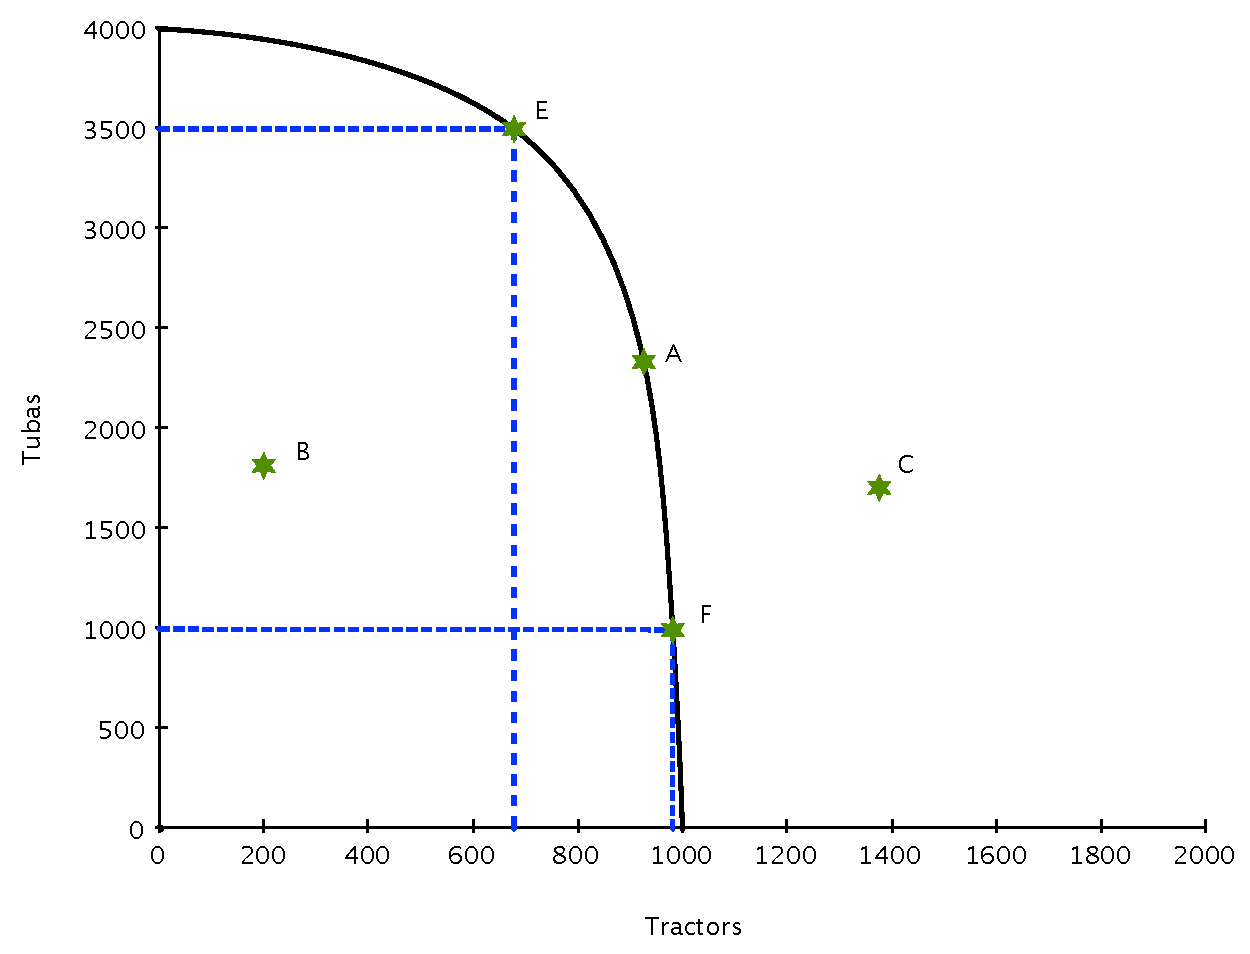
\includegraphics[scale=.40]{plot1.pdf}
			\caption{PPF for Tractors and Tubas}
			\label{ppf1}
		\end{figure}
	Why does it have this shape? \ddp{Specialization of resources.}
	\\
	
	At point \textbf{E}, the economy is using most of its resources to produce tubas and so the resources best suited to producing tractors are being used in the tuba industry. Thus, when we increase tractor production by one unit, we will only see a slight reduction in the number of tubas produced. 
	\\
	
	However, at point \textbf{F}, the resources best suited to producing tractors are already employed in that industry. Producing an additional tractor means moving resources more suited to producing tubas out of the tuba industry and thus there will be a large loss in the production of tubas.
	\\
	
	\ddp{Specialization of resources leads to increasing opportunity costs along the PPF.\\}
	
	Point \textbf{A} is said to be \dd{efficient}. 
	\ddp{The economy is producing all it can given its resources.}
	\\
	
	Point \textbf{B} is said to be \dd{inefficient}. 
	\ddp{The economy is not producing all it can given its resources (e.g., underemployment of workers, available land not being utilized).}
	\\
	
	Point \textbf{C} is said to be \dd{unfeasible}. 
	\ddp{The economy cannot support this output level with its current resources and technology.}
	\end{exmp}
	
	The PPF shows the first two principles of economics. In order to produce more tractors, you have to give up some tubas - society faces a trade-off. It also shows the opportunity cost of each good. 
	\\
	
	What does the slope of the PPF tell you? The reciprocal of the slope?
	\blank{}
	\ddp{\\ The slope of PPF is the OC of good on the x-axis. The reciprocal of the slope is the OC of good on the y-axis.}
	
	\subsubsection*{Shifts of the PPF}
	
	\begin{enumerate}
		\item Changes in the factors of production.
			
		\item Changes in technology.
		
	\end{enumerate}
	
	\ddp{Reemployment of existing resources does not shift the PPF. This will either move us along the PPF or between points within it.}
	
	\begin{exmp} For each of the following, draw what would happen to the PPF.
		\begin{enumerate}
			\item The economy experienced a technological advance in the production of tractors.
			\ddp{\\ The PPF will shift out at the x-axis since the economy can produce more tractors than before. The number of tubas it can produce is still the same.}
			\begin{figure}[H]
				\centering
				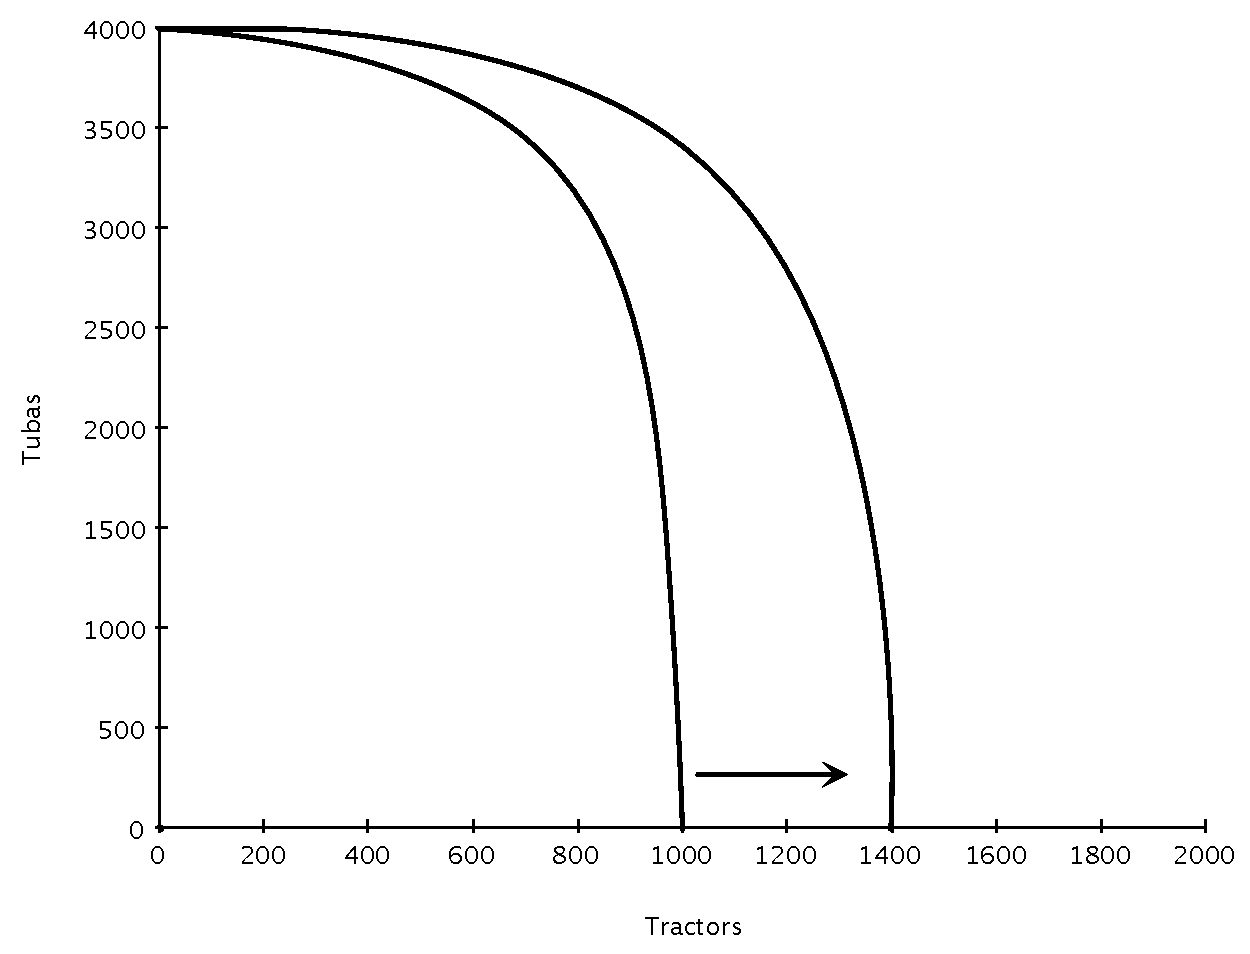
\includegraphics[scale=.40]{plot2.pdf}
				\caption{PPF Example 1}
				\label{ppf2}
			\end{figure}
			\item The country relaxed migration restrictions and saw an influx of more workers.
			\ddp{\\ The PPF will shift out at each axis since the economy can produce more of each good than before (available resources increased).} 
				\begin{figure}[H]
					\centering
					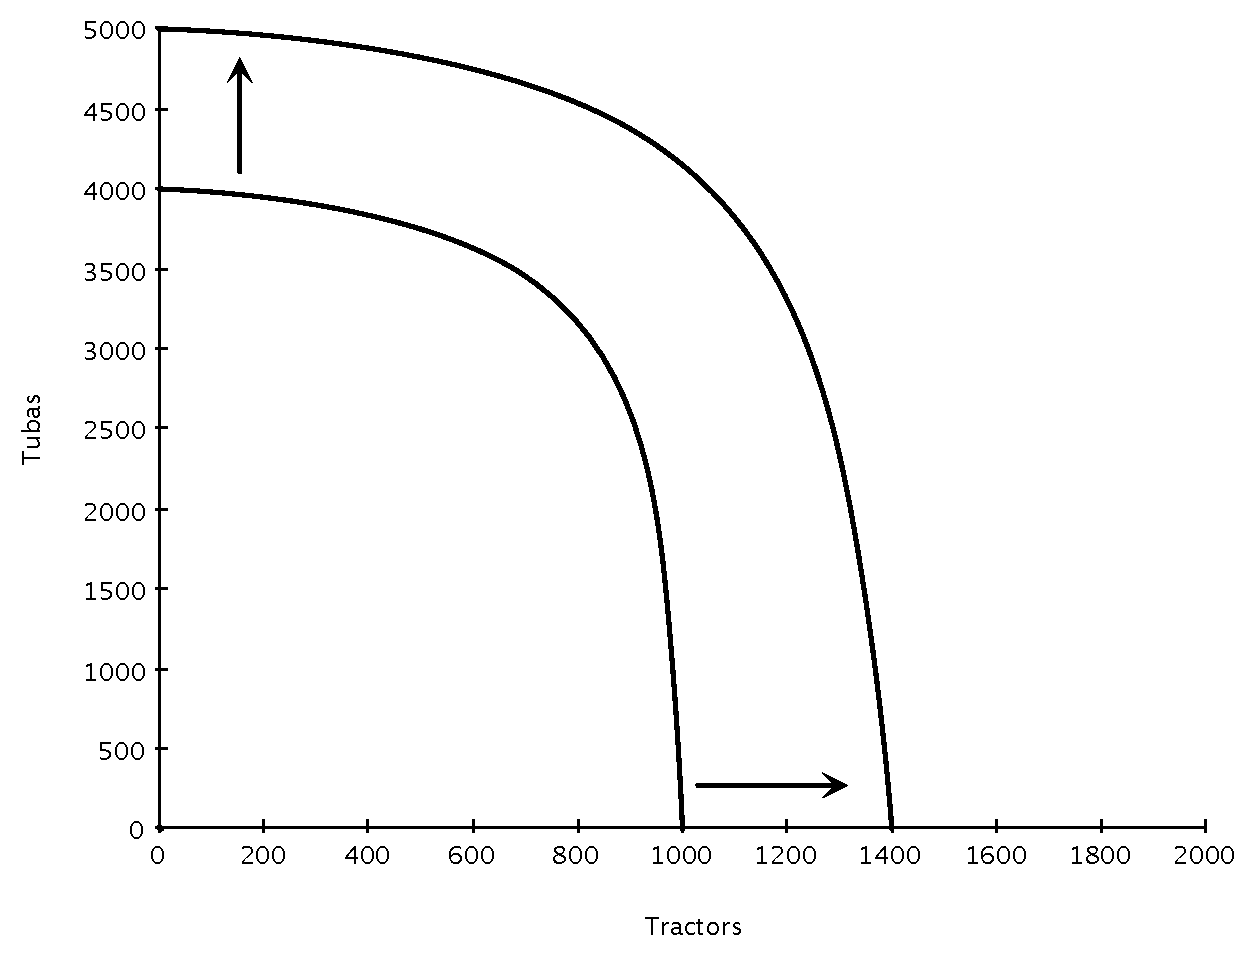
\includegraphics[scale=.40]{plot3.pdf}
					\caption{PPF Example 2}
					\label{ppf3}
				\end{figure}
		\end{enumerate}
	\end{exmp} 



	\subsubsection*{Simplifying the PPF}
	Changing the assumptions of the model such that resources are no longer specialized (i.e., worker skills are perfectly transferable across sectors) would cause the PPF to look as follows:
	\begin{figure}[H]
		\centering
		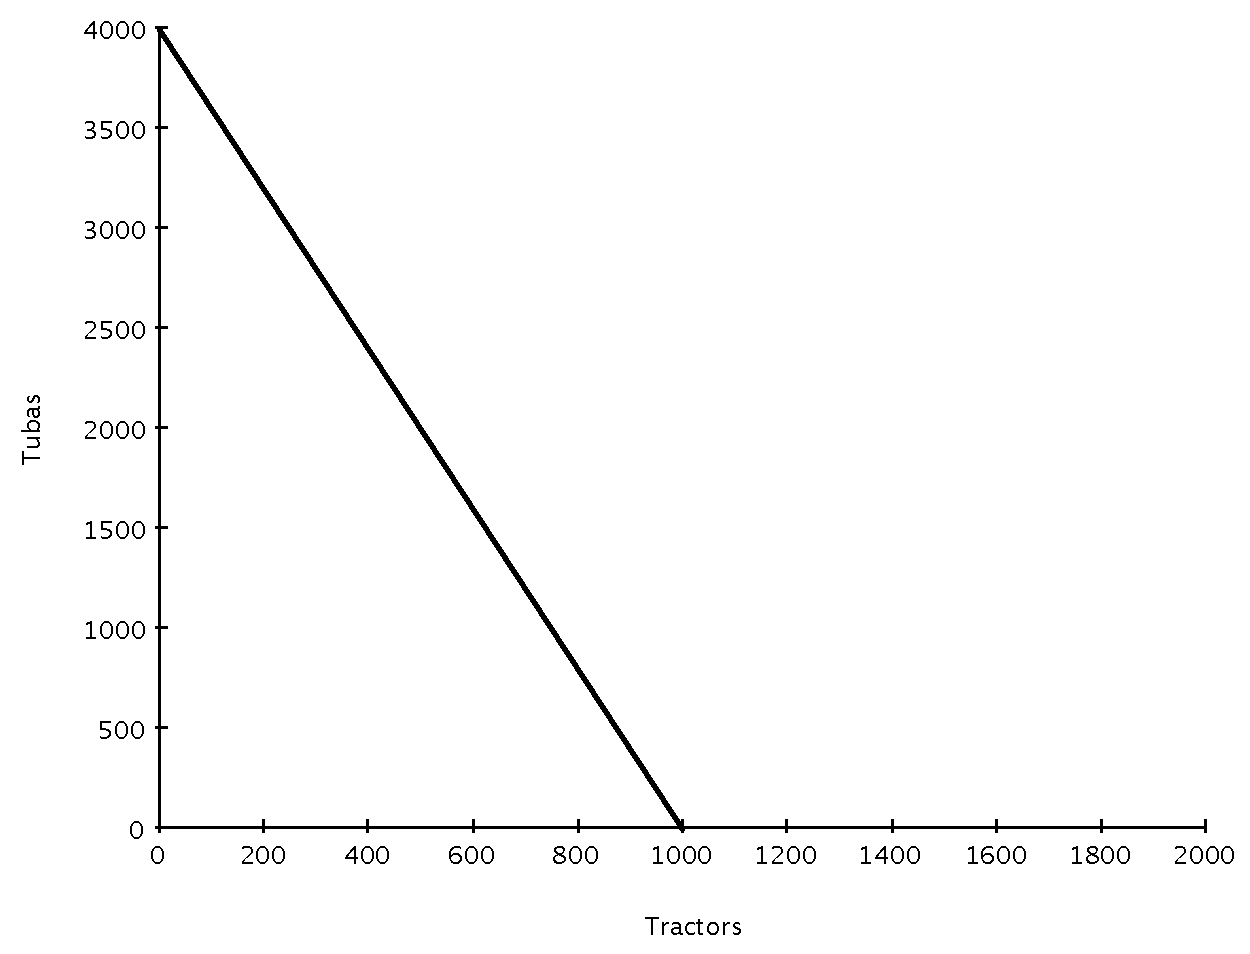
\includegraphics[scale=.40]{plot4.pdf}
		\caption{Straight-Line PPF}
		\label{ppf4}
	\end{figure}
	
	This is sometimes referred to as a straight-line PPF. Since the slope of the PPF is constant, the opportunity cost of each good is \dd{constant}. The (absolute) slope of the PPF gives the opportunity cost of the good on the \dd{x-axis}, while the reciprocal of the slope gives the opportunity cost of the good on the \dd{y-axis}.
	
\newpage
	
	\section{Interdependence and the Gains from Trade}	
	
	\textbf{Principle 5: Trade Can Make Everyone Better Off}
	\\
	
	Trade allows countries (or people) to specialize in what they do best and enjoy a greater variety of good and services.
	
	\subsection{Ratios and Unit Conversion}

	
	\begin{exmp}
		Express the ratio $25$ apples $: 75$ oranges in three different ways.
		\blank{}
	\end{exmp}
	\ddp{$1a : 3o$, $1/3a : 1o$, $50a : 150o$, etc.}
	
	\begin{exmp} 
		Josh takes 12 hours to produce 25 coconuts. How many coconuts can he produce in one day? In one week?
		\blank{}
	\end{exmp} 
	\ddp{25 coconuts/12 hours $\times$ 24 hours/day = 50 coconuts/day. 50 coconuts/day $\times$ 7 days/week = 350/week.}

	
	\begin{exmp} 
		Instead of coconuts, Josh can use his time to produce pineapples. In 12 hours, he can produce 5 pineapples. If he uses his whole day to produce coconuts, how many pineapples is he giving up? What is his opportunity cost of producing one coconut?
		\blank{}
	\end{exmp}
	\ddp{Can produce 5 pineapples/12 hours $\times$ 24 hours/day = 10 pineapples/day. Per day, he gives up 10 pineapples to produce 50 coconuts. Ratio: 10 pineapples : 50 coconuts $\Rightarrow$ 1 coconut : 1/5 pineapple. OC of 1 coconut is 1/5 a pineapple.}

	
	
	\subsection{Absolute Advantage}
	
	\defn{Absolute Advantage:} 
	\ddp{\begin{itemize}
			\item The ability to produce a good using fewer inputs than another producer.
			\item The ability to produce more units of a good using the same number of inputs.
		\end{itemize}}
	
	\begin{exmp}
		Pepe can grow 25 potatoes in one day, while Silvia can grow 20 potatoes in a day. Who has an absolute advantage in the production of potatoes? Why?
		\blank{}
	\end{exmp} 
	\ddp{Pepe has AA because he can produce more potatoes than Silvia using the same number of inputs (1 day).}
	
	\begin{exmp} 
		The following table shows the production possibilities available to Harold and Kumar:
	
	\begin{table}[H]
		\caption*{Minutes needed to make 1 ounce of:}
		\centering
		\begin{tabular}{c|c|c|}
			
			& Beans & Porridge \\
			\hline
			Harold & 20 min/oz & 15 min/oz \\
			
			Kumar  & 30 min/oz & 60 min/oz \\
			
		\end{tabular}
	\end{table}
	
	Who has an absolute advantage in the production of beans? Of porridge? Why?
	\end{exmp}
	\ddp{Harold has an AA in both goods because she can produce 1 oz of each good using fewer inputs than Kumar.}
	\blank{}
	
	\subsection{Comparative Advantage}
	
	\defn{Comparative Advantage:} \ddp{The ability to produce a good at a lower opportunity cost than another producer.}
	
	\begin{exmp}
		Instead of potatoes, Pepe \& Silvia could produce yuccas. Pepe can grow 50 yuccas in a day and Silvia can grow 80. What is the opportunity cost of 1 potato for Pepe? For Silvia? Who has the comparative advantage in the production of potatoes?
		\blank{} \blank{}
	\end{exmp} 
	\ddp{Pepe: 25 P : 50 Y $\Rightarrow$ 1 P : 2 Y, 1 Y : 1/2 P.\\
		Silvia: 20 P : 80 Y $\Rightarrow$ 1 P : 4 Y, 1 Y : 1/4 P. \\
		Pepe has CA in potatoes, Silvia has CA in yuccas.}
	
	\begin{exmp}
		What is the opportunity cost of 1 ounce of beans for Harold? For Kumar? What is the opportunity cost of 1 ounce of porridge for each? Who has the comparative advantage in each good?
		\blank{} \blank{}
	\end{exmp} 
	\ddp{Harold: 20 min/1 oz beans : 15 min/1 oz porridge $\Rightarrow$ 1 oz beans/20 min : 1 oz porridge/15 min $\Rightarrow$ 1 oz beans : 1.33 oz of porridge, 1 oz porridge : .75 oz beans. \\ \\
		Kumar: 30 min/1 oz beans : 60 min/1 oz porridge $\Rightarrow$ 1 oz beans/30 min : 1 oz porridge/60 min $\Rightarrow$ 1 oz beans : 1/2 oz of porridge, 1 oz porridge : 2 oz beans. \\ \\
		Kumar has CA in beans, Harold has CA in porridge. \\}

	
	It is possible for one person to have an absolute advantage in both goods. But it is impossible to have a comparative advantage in both goods because the opportunity cost of one good is the \dd{reciprocal} of the other. If the opportunity cost of one good is relatively high, the opportunity cost of the other good must be relatively low. 
	\\
	
	Unless the two parties have the same opportunity cost, one person will have a comparative advantage in one good, and the other will have a comparative advantage in the other.
	
	\subsection{The Gains from Trade}
	
	The gains from trade are based on \dd{comparative advantage}. That is, when each party specializes in producing the good for which they have a  \dd{lower opportunity cots}, total production in the economy increases. 
	\\
	
	To illustrate this, let's use an example with Pepe and Silvia.
	
	\begin{table}[H]
		\caption*{Daily production of potatoes and yucca:}
		\centering
		\begin{tabular}{ c|c|c|}        
			
			& Potatoes & Yuccas \\
			\hline
			Pepe & 25 & 50  \\
			
			Silvia  & 20 & 80  \\
			
		\end{tabular}
	\end{table}
	
		\begin{figure}[h!]
			\centering
			\caption{The Gains from Trade}
			\begin{subfigure}{.5\textwidth}
				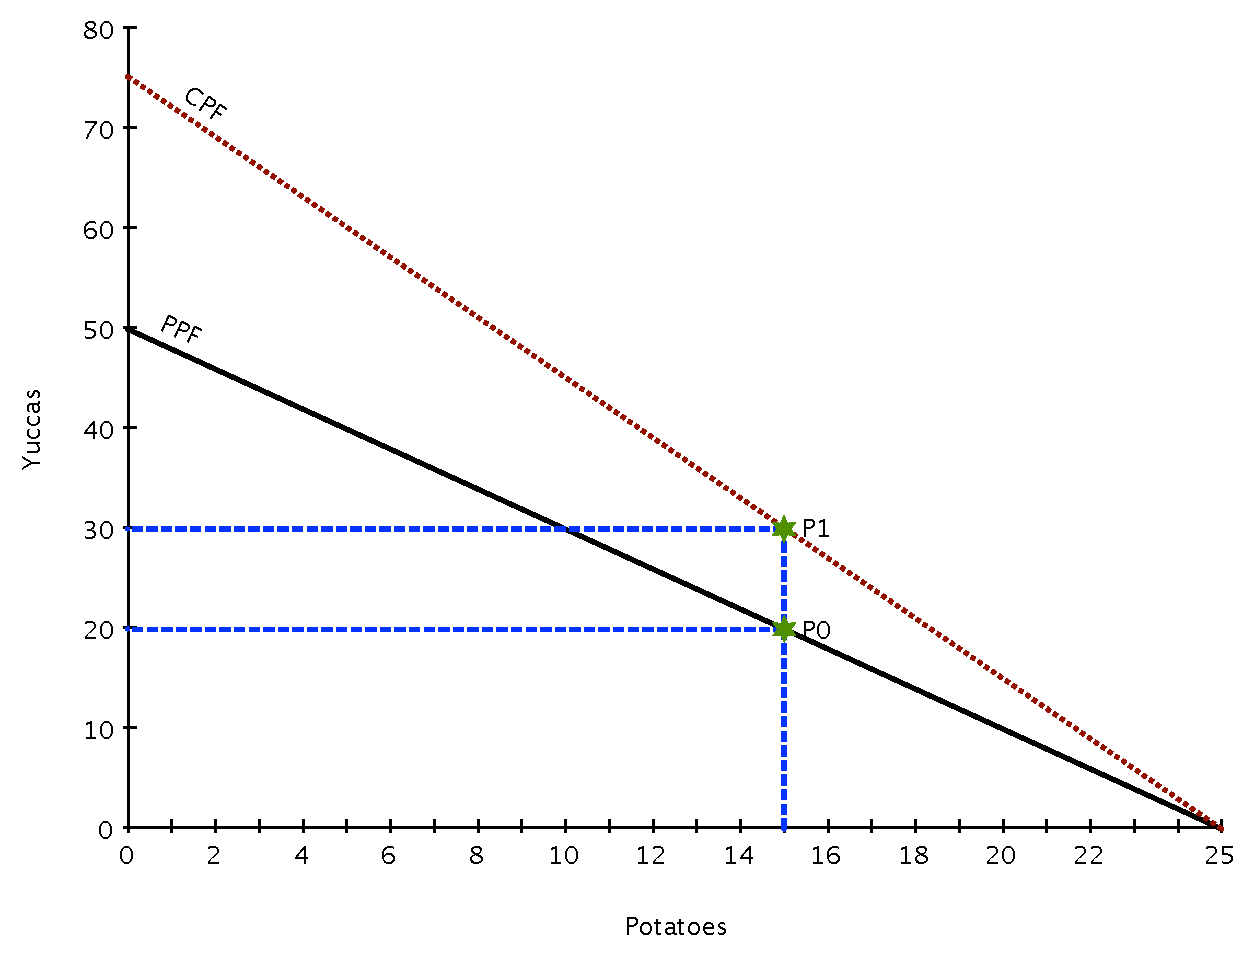
\includegraphics[scale=.3]{plot5.pdf}
				\caption{Pepe's PPF}
			\end{subfigure}%
			\begin{subfigure}{.5\textwidth}
				\centering
				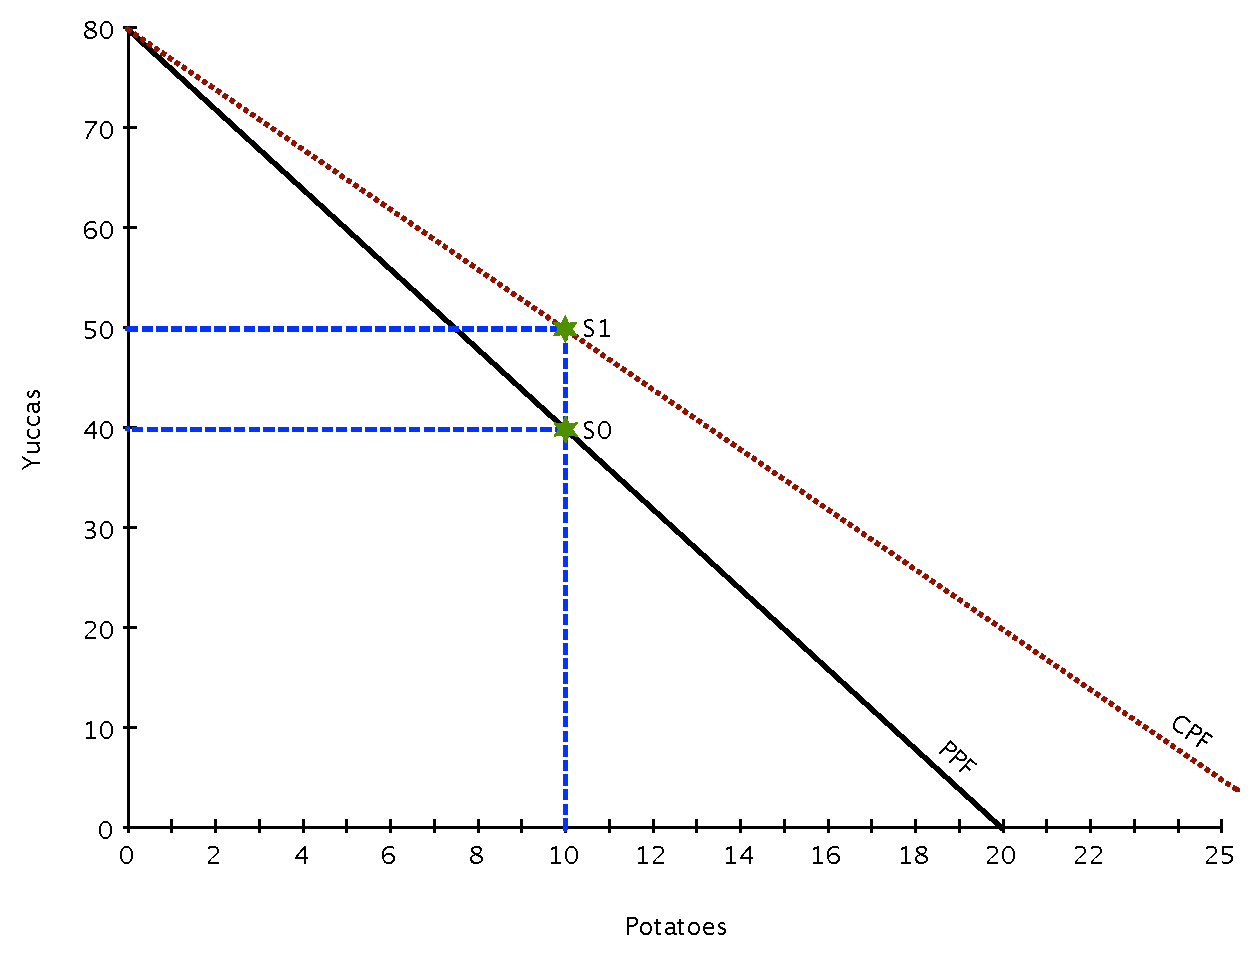
\includegraphics[scale=.3]{plot6.pdf}
				\caption{Silvia's PPF}
			\end{subfigure}
		\end{figure}
	
	
	Suppose that currently, Pepe produces and consumes 15 potatoes while Silvia produces and consumes 10 potatoes. With no trade, if both are operating at efficient points, this means that Pepe is producing and consuming \dd{20} yuccas while Silvia is producing and consuming \dd{40} yuccas. 
	
	\ddp{\\ Pepe is producing 15 potatoes, so is giving up 15 potatoes $\times$ 2 yuccas/potato = 30 yuccas. So, he is consuming 50 - 30 = 20 yuccas. \\ \\
		Silvia is giving up 10 potatoes $\times$ 4 yuccas/potato = 40 yuccas. So consuming 80 - 40 = 40 yuccas. \\}
	\blank{} \blank{}
	
	Denote these points $P_0$ and $S_0$ on their respective PPFs. Thus, between them, they are currently producing 25 potatoes and \dd{60} yuccas.
	\\
	
	Pepe has a comparative advantage in potatoes and Silvia has a comparative advantage in yuccas. Therefore with trade, Pepe will export \dd{potatoes} to Silvia and import \dd{yuccas}. 
	\\
	
	Suppose that Pepe and Silvia decide to exchange 1 potato for 3 yuccas. This is their so-called ``terms of trade.''
	\\
	
	What happens to their production and consumption if they decide trade 10 potatoes for yuccas?
	
	\ddp{\\ Pepe: Produces 25 potatoes, exports 10 in exchange for 10 potatoes $\times$ 3 yuccas/potato = 30 yuccas. Consumption of yuccas increased due to trade. \\ \\
		Silvia: Produces 80 yuccas, exports 30 in exchange for 10 potatoes. \\ 
		Without trade, would give up 50 yuccas $\times$ 1 potato/4 yuccas = 12.5 potatoes and so consume 20 - 12.5 = 7.5 potatoes. Consumption of yuccas increased due to trade.\\}
	\blank{} \blank{}
	
	Pepe can now consume at point $P_1$ and Silvia can consume at point $S_1$, which were impossible without trade. Total production in the economy is now 25 potatoes and 80 yuccas, so total production increased as well.
	\\
	
	Thus, comparative advantage and specialization allow for \dd{increased} consumption by \textbf{both} parties and increased total production in the economy. 
	
	\subsection{The Price of Trade}
	
	In order for trade to be beneficial, it must make both parties better off. In order to do so, the terms of trade must lie between the \dd{opportunity costs} of each party. 
	\\
	
	Consider Pepe and Silvia's trade from the perspective of each party:
	\\
	
	\textit{Pepe's perspective:}
	\ddp{Exports potatoes in exchange for yuccas. On his own, Pepe gives up 2 yuccas for each potato. Thus, he is only better off if he receives \underline{more} than 2 yuccas for each potato he exports. \\}
	\blank{} \blank{}
	
	\textit{Silvia's perspective:}
	\ddp{Imports potatoes in exchange for yuccas. On his own, Silvia gives up 4 yuccas for each potato. Thus, he is only better off if he gives up \underline{less} than 4 yuccas for each potato he imports.\\} 
	\blank{} \blank{}
	
	Thus, if expressing the terms of trade as 1 potato $: X$ yuccas, it has to be that \dd{2} $< X <$ \dd{4} in order for both parties to be better off.
	
	\newpage
	
	\section{Supply and Demand}
	
	\subsection{Markets and Competition}
	
	\defn{Market:} \ddp{A group of buyers and sellers of a particular good or service.\\}
	
	\defn{Competitive Market:} \ddp{A market in which there are many buyers and many sellers so that each has negligible impact on the market price.\\}
	
	For the next few chapters, we will focus on markets that are \textbf{perfectly competitive.} 

	\ddp{\\ Goods are exactly the same, buyers \& sellers are price takers. Other types: monopolies, oligopolies. We will study those later.}
	
	
	\subsection{Demand}
	
	\defn{Quantity Demanded:} \ddp{The amount of a good or service that buyers are willing and able to purchase.}
	
	\begin{exmp}
		Table \ref{tab1} below shows how many used economics textbooks students in this class are willing to buy at different prices.
	\begin{table}[ht]
		\caption{David's Class}
		\label{tab1}
		\centering
		\begin{tabular}{  c| c}        
			
			Price   & Quantity Demanded \\
			\hline
			\$60 & 0 \\
			\$50 & 3 \\
			\$40 & 6 \\
			\$30 & 9 \\
			\$20& 12 \\
			\$10 & 15 \\
			\$0 & 18 \\
		\end{tabular}
	\end{table} 
	
	This kind of table is referred to as a \dd{demand schedule}. From this table, draw the \textbf{demand curve} for this market.
	\end{exmp}
	
		\begin{figure}[H]
			\centering
			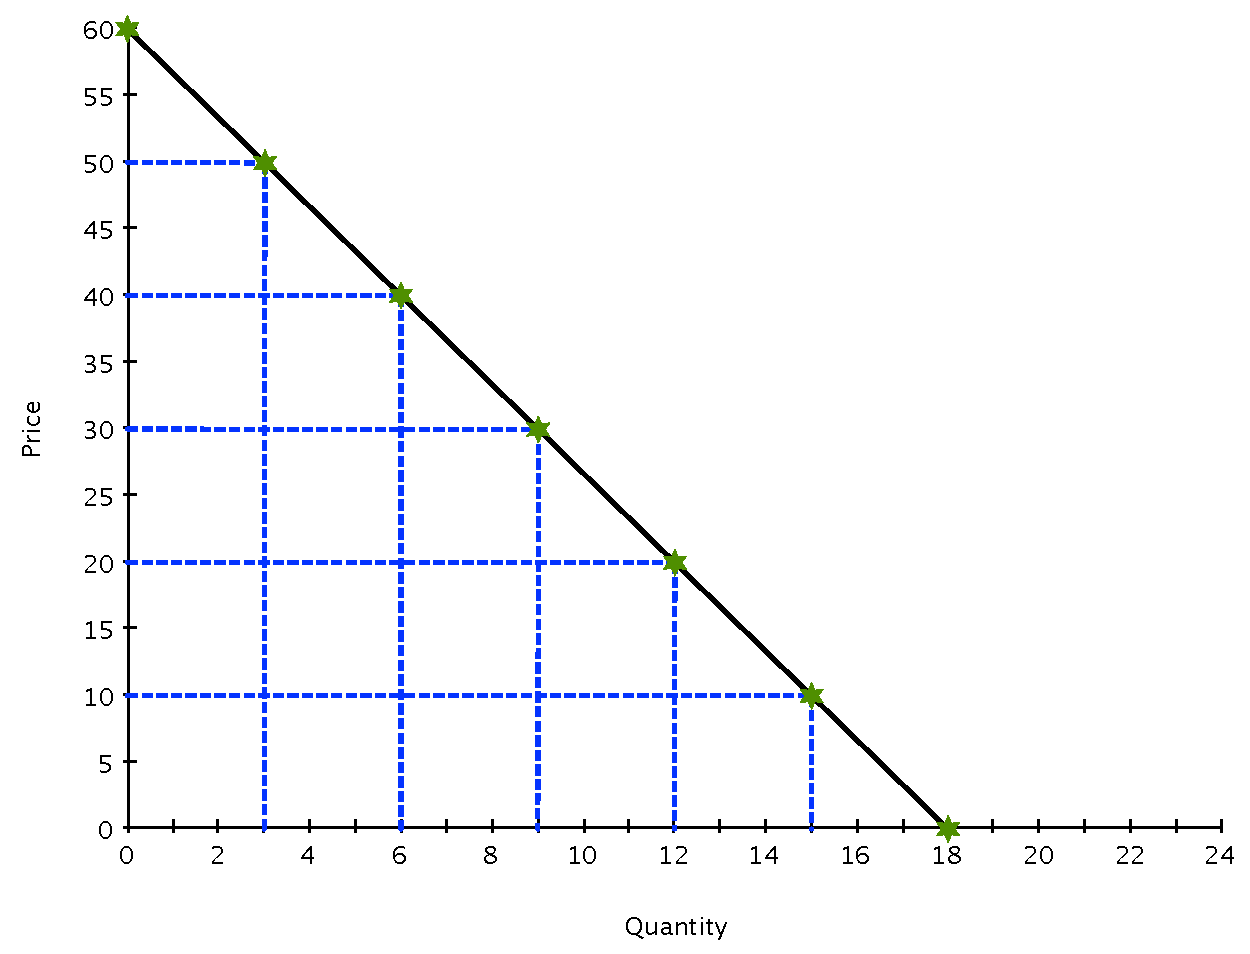
\includegraphics[scale=.35]{plot7.pdf}
			\caption{Demand for Textbooks}
		\end{figure}
		
	Notice that by convention, we plot \dd{prices} on the y-axis and \dd{quantity} on the x-axis.
	\\
	
	Both the table and the curve demonstrate the \defn{law of demand.}
	
	\ddp{\\ All else equal, the quantity demanded of a good increases when the price of the good decreases.}
	
	\begin{exmp}
		
	Suppose student's in Wenting's Econ 101 class are willing to buy used textbooks according to Table \ref{tab2}.
	
	\begin{table}[ht]
		\caption{Wenting's Class}
		\label{tab2}
		\centering
		\begin{tabular}{  c|c}        
			
			Price   & Quantity Demanded \\
			\hline
			\$60 & 2 \\
			\$50 & 4 \\
			\$40 & 6 \\
			\$30 &  8 \\
			\$20& 10 \\
			\$10 & 12 \\
			\$0 & 14 \\
		\end{tabular}
	\end{table} 
	
	If these two classes make up the market for used economics textbooks at UNC, what is the market quantity demanded at each price? Draw the market demand curve.
		
			\begin{figure}[H]
				\centering
				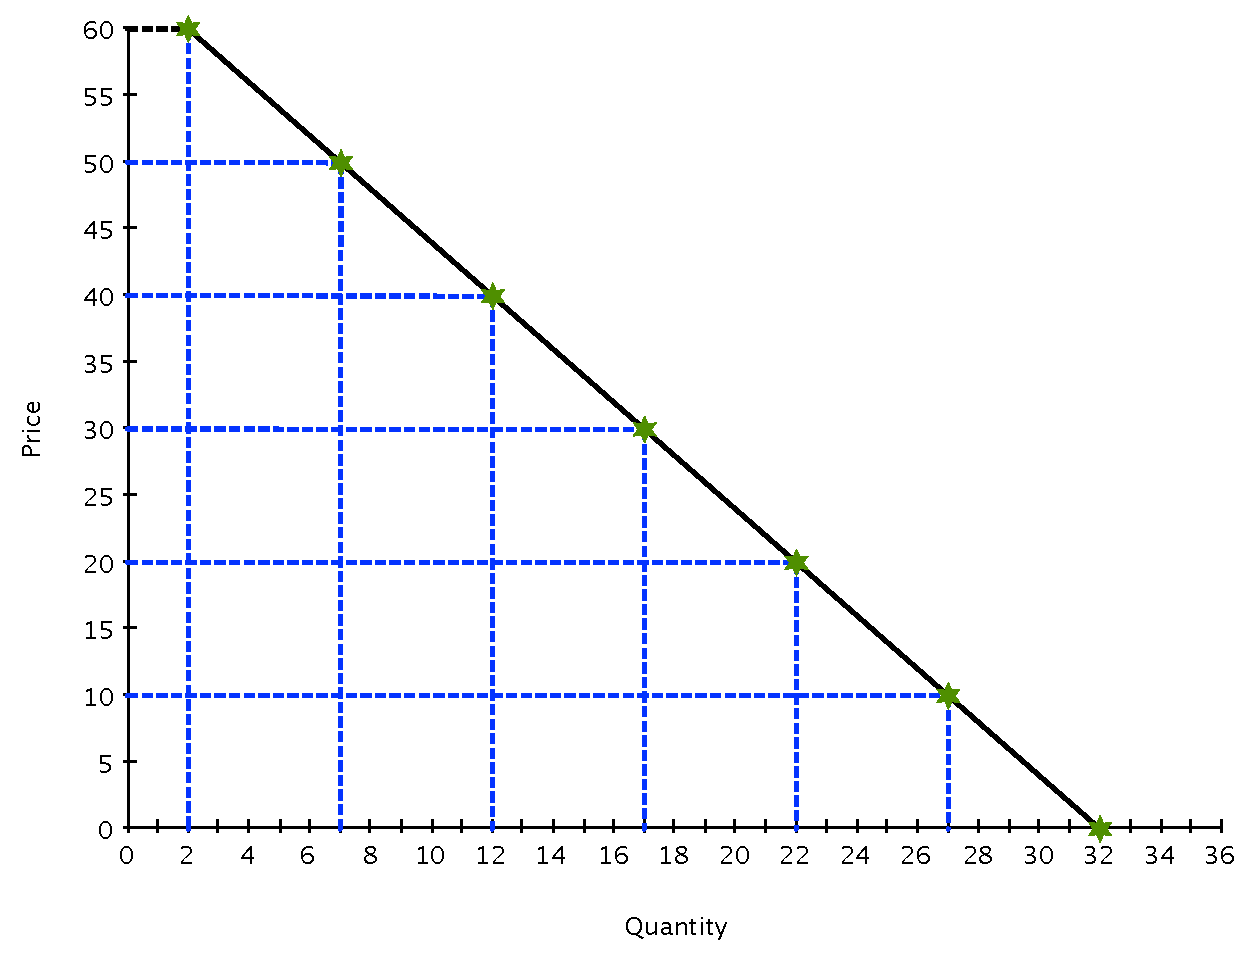
\includegraphics[scale=.35]{plot8.pdf}
				\caption{Demand for Textbooks}
			\end{figure}
			
	If the price of used economics textbooks is \$40, how many books will be demanded? What if the price increased to \$50? Notice that this change in price caused \dd{a movement along the demand curve}.
	\end{exmp}
	
	The demand curve holds everything but price and quantity demanded constant. But there are other things that affect how much people are willing to purchase at any given price. Changes in these factors cause \dd{shifts} of the demand curve. 
	\\
	
	This is referred to as a \dd{change in demand}.
	\blank{}
	\blank{}
	\blank{}
	\blank{}
	\blank{}
		

	
		\begin{figure}[H]
			\centering
			\caption{Shifts in Demand}
			\begin{subfigure}{.5\textwidth}
				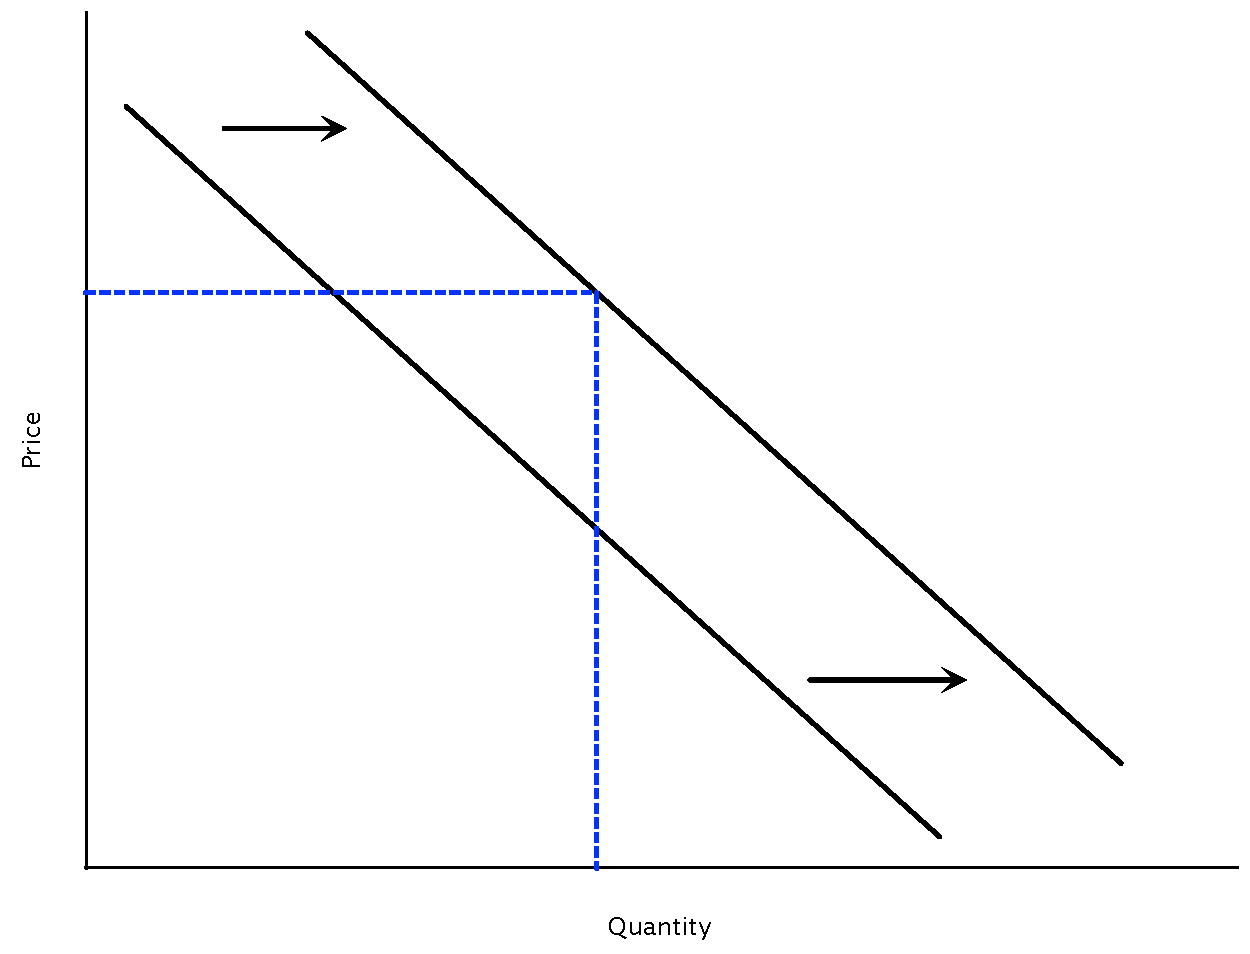
\includegraphics[scale=.3]{plot9.pdf}
				\caption{Increase in Demand}
			\end{subfigure}%
			\begin{subfigure}{.5\textwidth}
				\centering
				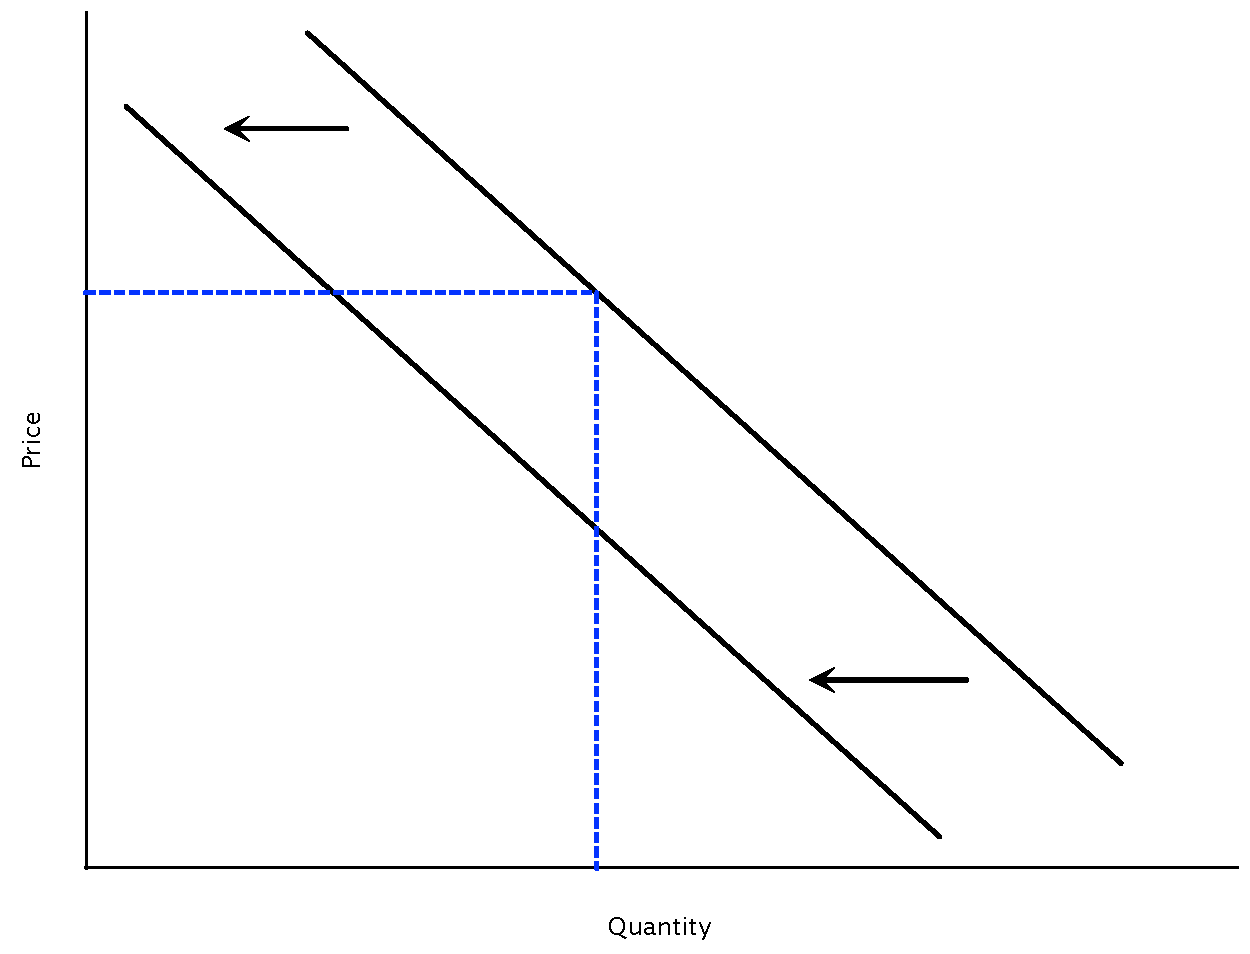
\includegraphics[scale=.3]{plot10.pdf}
				\caption{Decrease in Demand}
			\end{subfigure}
		\end{figure}
	
	\begin{itemize}
	\setlength\itemsep{1.5em}
		\item Increase in demand: \ddp{ \\ Horizontal reading: At any given price, willing and able to purchase more. \\ \\ Vertical: At any given quantity, willing and able to pay more. We would say demand ``increases'' or demand ``shifts right.''}
		\item Decrease in demand: \ddp{\\ Horizontal reading: At any given price, willing and able to purchase less.\\ \\ Vertical: At any given quantity, willing and able to pay less. We would say demand ``decreases'' or demand ``shifts left.''}
	\end{itemize}
	
	\subsubsection*{Variables that Shift the Demand Curve:}

	\begin{enumerate}
		\item Income
	\end{enumerate}
	
	\hspace{.5cm} \defn{Normal good:} \ddp{A good for which an increase in income leads to an increase in demand. This describes most goods. \\}

	
	\hspace{.5cm} \defn{Inferior good:} \ddp{A good for which an increase in income leads to a decrease in demand (e.g., ramen soup).}

	
	\begin{enumerate}
		\setcounter{enumi}{1}
		\item Prices of related goods
	\end{enumerate}
	
	\hspace{.5cm} \defn{Substitutes:} \ddp{Goods for which an increase in the price of one leads to an increase in demand for the other (e.g., coffee \& tea, coke \& pepsi, bud light \& coors light). \\}
	
	\hspace{.5cm} \defn{Complements:} \ddp{Goods for which an increase in the price of one leads to a decrease in demand for the other (e.g., hot dogs and hot dog buns, pizza and beer).}
	
	\begin{enumerate}
		\setcounter{enumi}{2}
		\setlength{\itemsep}{15pt}
		\item Tastes: \ddp{Perceptions of products affects how in-demand they are. News, cultural changes, etc. will change preferences.}
		\item Expectations: \ddp{Expected future prices affect current demand. If prices are predicted to increase in the future, then demand today will increase. If prices are predicted to decrease, demand today will decrease.}
		\item Number of buyers: \ddp{More buyers $\Rightarrow$ more demand.}
	\end{enumerate}
	
	

	\begin{exmp}
	Consider the demand for cigarettes. What happens in each of the following scenarios? Explain why.
	\begin{enumerate}
	\setlength{\itemsep}{1em}		
	\item	The surgeon general declares that cigarettes are even more harmful than previously believed.
 
	\ddp{Change in tastes. Demand decreases.}
	
	
	\item	Individuals start believing a rumor that the government is going to raise the cigarette tax by \$1.00.
 
	\ddp{Expected future price increases. Demand today will increase.}
	
	
	\item 	The price of beer increases. 

	\ddp{Assuming they are complements, an increase in the price of beer will drive demand for cigarettes down.}

	
	\item 	The price of cigarettes decreases.  
	
	\ddp{Demand doesn't shift. A change in price leads to a movement along the demand curve.}
\end{enumerate}
	\end{exmp}

	\subsection{Supply}
	
	\defn{Quantity Supplied:} \ddp{The amount of a good that sellers are able and willing to sell.\\}

	\defn{Law of Supply:} \ddp{All else equal, the quantity supplied of a good rises when the price of the good rises.\\}
	
	\defn{Supply Schedule:} \ddp{A table that shows the relationship between the price of a good and the quantity supplied.\\}
	
	\defn{Supply Curve:} \ddp{A graph that shows the relationship between the price of a good and the quantity supplied, holding constant everything else that influences how much sellers of the good want to sell.\\}
	
	\defn{Market Supply:} \ddp{The sum of all the individual supplies for a particular good or service.\\}
	
	Just like the demand curve, the supply curve holds everything but price and quantity constant. But there are other things that affect how much sellers are willing to sell at any given price. Changes in these factors cause shifts of the supply curve. Similar to demand, this is referred to as a shift in supply. 
	
	
	\begin{figure}[H]
		\centering
		\caption{Shifts in Supply}
		\begin{subfigure}{.5\textwidth}
			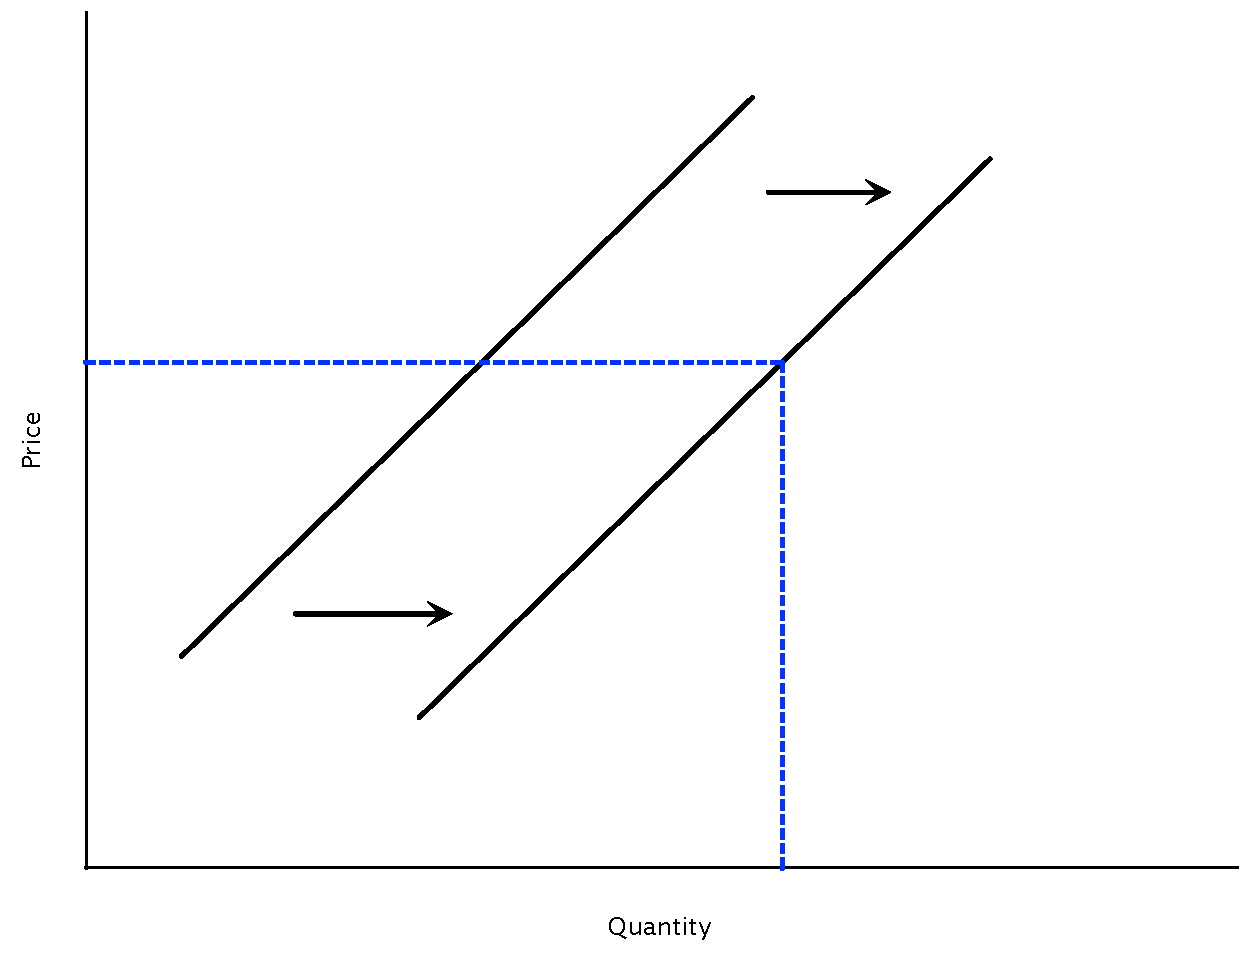
\includegraphics[scale=.3]{plot11.pdf}
			\caption{Increase in Supply}
		\end{subfigure}%
		\begin{subfigure}{.5\textwidth}
			\centering
			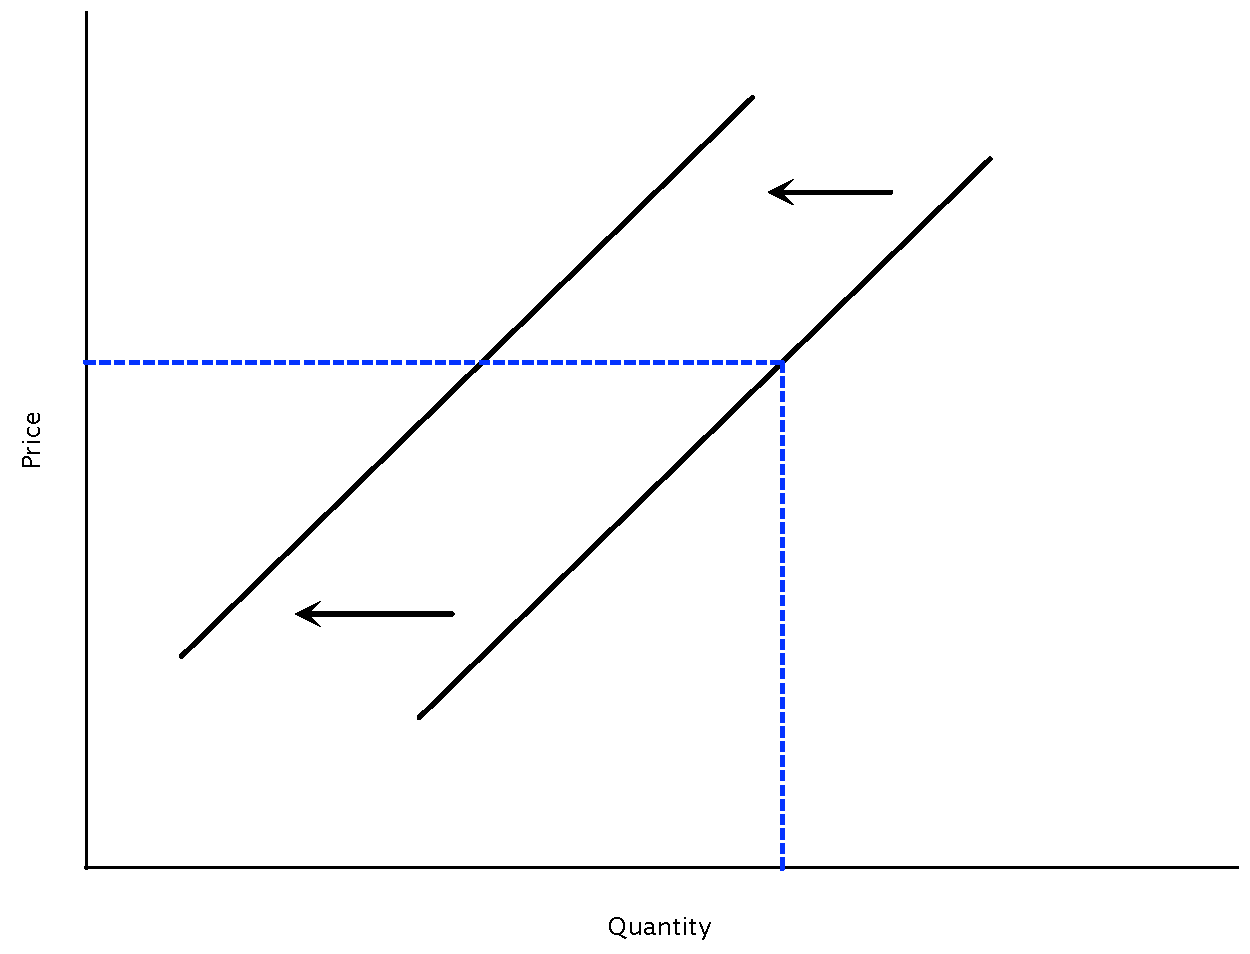
\includegraphics[scale=.3]{plot12.pdf}
			\caption{Decrease in Supply}
		\end{subfigure}
	\end{figure}

	\begin{itemize}
		\setlength{\itemsep}{1.5em}
		\item Increase in supply: \ddp{\\ Horizontal: At any given price, willing and able to sell more of a good. \\ \\
			Vertical: At any given quantity, willing to sell good for a lower price. \\ We'd say supply shifts right.}
		\item Decrease in supply: \ddp{\\ Horizontal: At any given price, willing and able to sell less of a good. \\ \\
			Vertical: At any given quantity, willing to sell good for a higher price. \\ We'd say supply shifts left.}
	\end{itemize}
	\vspace{.5em}
	
	\subsubsection*{Variables that Shift the Supply Curve:}
	
	\begin{enumerate}
		\setlength{\itemsep}{15pt}
		\item Input prices \ddp{\\ Higher input prices mean that suppliers must receive a higher price to sell any given quantity. Supply decreases. \\ Lower input prices imply sellers are willing to accept less to supply a given quantity. Supply increases.}
		\item Technology \ddp{\\ Advances in technology lower costs of production and thus allow firms to sell more for any given price. Supply increases.}
		\item Expectations \ddp{\\ If prices are expected to increase in the future, supply today will decrease. If prices are expected to decrease in the future, supply today will increaes.}
		\item Number of sellers \ddp{\\ More sellers $\Rightarrow$ Increase in supply.}
	\end{enumerate}
	
\begin{exmp}
	Consider the supply for cigarettes.  What happens in each of the following scenarios? Explain why.
	
\begin{enumerate}
	\setlength{\itemsep}{1em}
		\item The minimum wage is increased.

	\ddp{Min wage is an ``input price.'' Supply decreases.}

	\item	A new device is invented that harvests tobacco at $1/2$ the previous cost.

	\ddp{Better technology allows for more production. Supply increases.}
 
	\item 	The price of cigarettes increases.

	\ddp{Change in the price of the good leads to a movement along the curve. Supply stays the same, but the quantity demanded increases.}
 
	\item	An overseas cigarette manufacturer starts producing in America.

	\ddp{Increase in the number of sellers. Supply increases.}
	
\end{enumerate}
	\end{exmp}
	
\newpage	
	
	\section{Market Equilibrium and the Efficiency of Markets}
	
	\textbf{Principle 6: Markets are Usually a Good Way to Organize Economic Activity}
	\\
	
	\defn{Welfare Economics}: \ddp{The study of how the allocation of resources affects economic well-being.}
		
		\subsection{Market Equilibrium}
		
		\defn{Equilibrium:} \ddp{The point at which the market price is such that $Q_D = Q_S$.\\}
		
		\defn{Equilibrium price:} \ddp{The price that balances $Q_D$ and $Q_S$. Denoted $P^*$.\\}
		
		\defn{Equilibrium quantity:} \ddp{$Q_D$ and $Q_S$ at the equilibrium price. Denoted $Q^*$.\\}
		
			\begin{figure}[H]
				\centering
				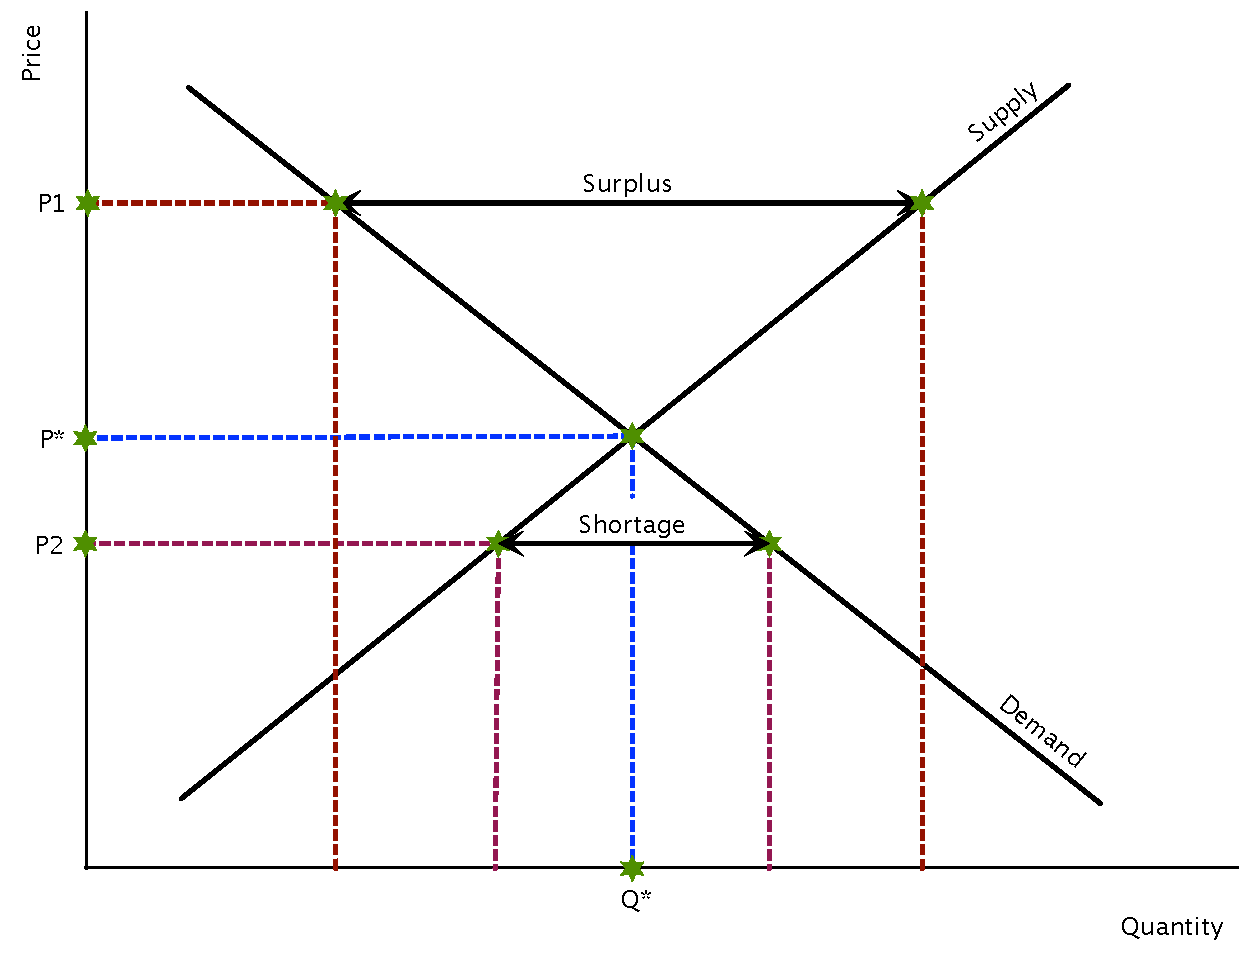
\includegraphics[scale=.40]{plot13.pdf}
				\caption{Market Equilibrium}
			\end{figure}
		
		
		Graphically, the equilibrium is given by point $E$, where the two curves intersect. $P^*$ and $Q^*$ denote the equilibrium price and quantity, respectively.
		\\
		
		What if the market price was $P_1$? At this price, we  have that \dd{quantity supplied} is greater than \dd{quantity demanded}. This is referred to as a \dd{surplus}. There will be \dd{downward} pressure on prices. These changes in prices represent movements \textit{along} the supply and demand curves.
		\\
		
		What if the market price was $P_2$? At this price, we would have that \dd{quantity demanded} is greater than \dd{quantity supplied}. This is referred to as a \dd{shortage}. In this scenario, there is \dd{upward} pressure on prices. 
		\\
		
		Importantly, no matter what the price is originally, the activities of the buyers and sellers automatically push the market price toward the equilibrium price.
		\\
		
		\defn{The Law of Supply and Demand:} \ddp{The price of a good adjusts to bring the quantity demanded and quantity supplied for that good into balance. \\}


		\begin{exmp}	Consider the market for cigarettes. For each of the following scenarios, draw any shifts in supply and/or demand.
		\begin{enumerate}
		
	
		\item	A drought hits tobacco-producing states. What situation are we in after the shift occurs, but before prices adjust?
		
		\ddp{Supply decreases. The equilibrium price increases and equilibrium quantity falls. Before the price adjustment, the market is facing a shortage because the price is too low.}
		
			\begin{figure}[H]
				\centering
				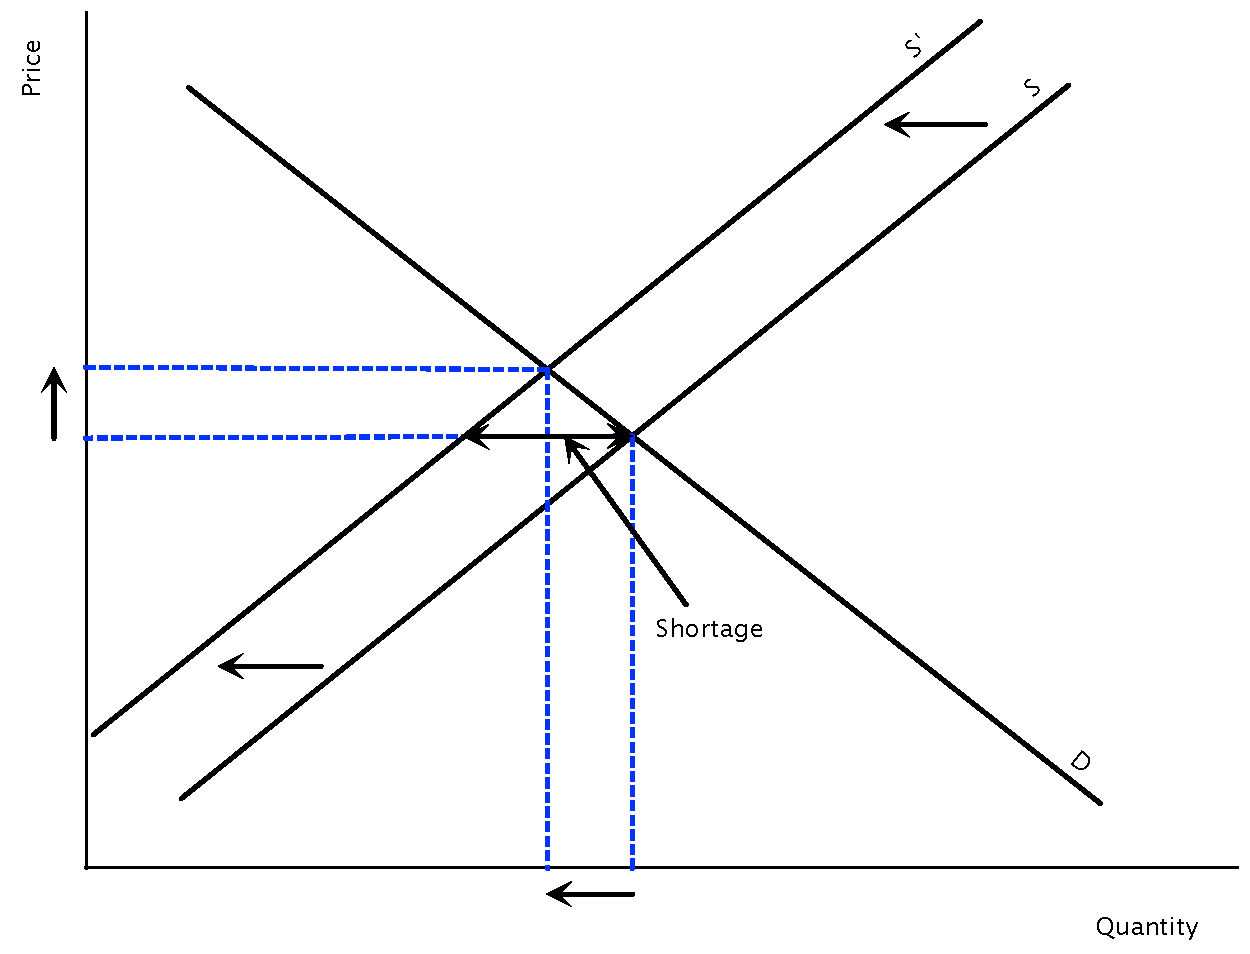
\includegraphics[scale=.30]{plot14.pdf}
				\caption{Example 4.1.1}
			\end{figure}
			

		\item 	Individuals start believing a rumor that the government is going to raise the cigarette tax by \$1.00.
		
		\ddp{The EFP increases. Assuming only demand is affected, demand today will increase. The equilibrium price and quantity will both increase.}
	
		\begin{figure}[H]
			\centering
			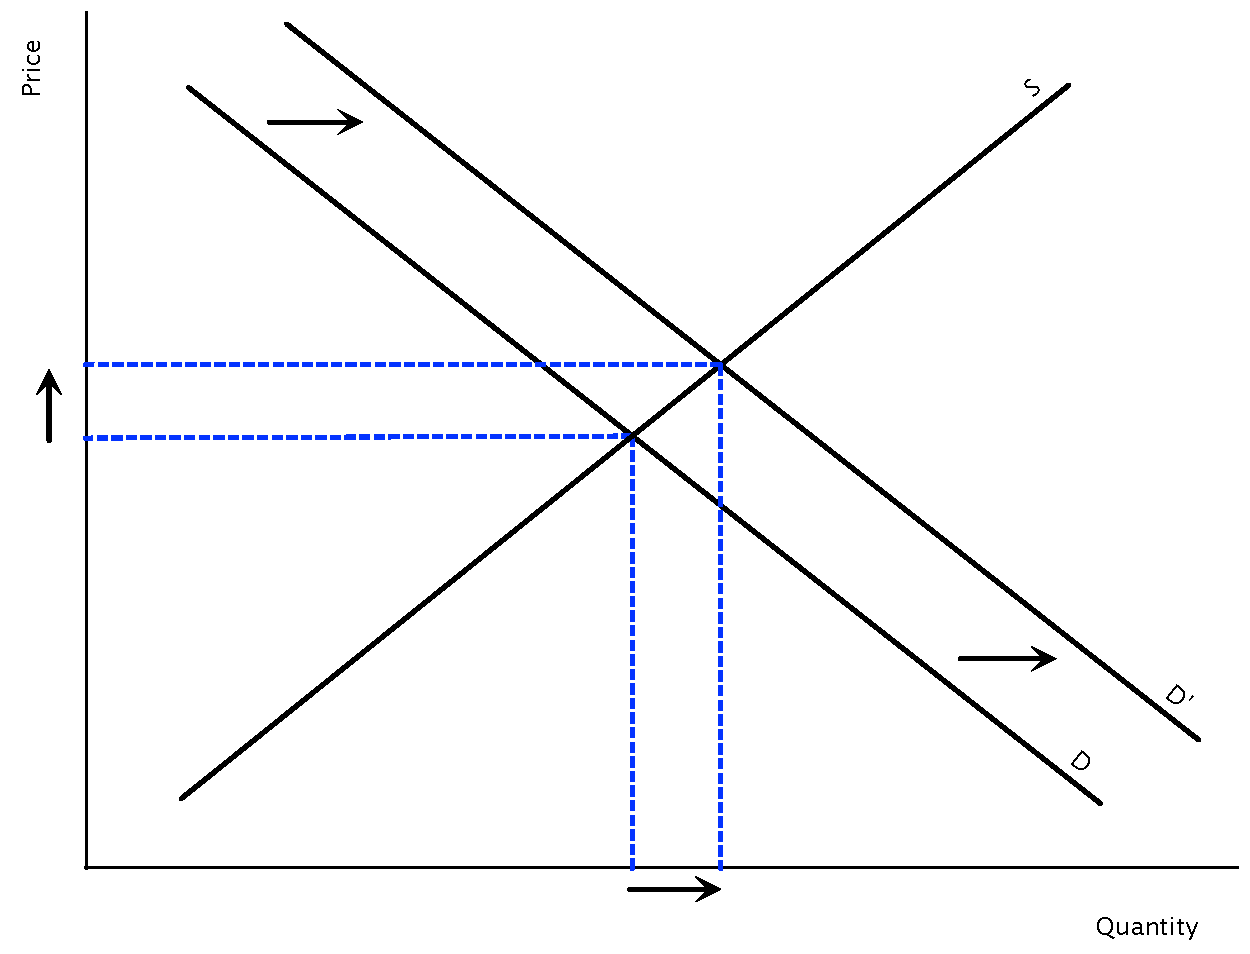
\includegraphics[scale=.30]{plot15.pdf}
			\caption{Example 4.1.2}
		\end{figure}
		
		
	
		\item 	An overseas cigarette manufacturer starts producing in America. Simultaneously, the surgeon general announces cigarettes are more harmful than previously believed.
	 
		\ddp{1. Increase in \# of sellers increases supply. The equilibrium price falls and equilibrium quantity increases. \\ 
			2. Demand falls. The equilibrium price decreases and equilibrium quantity falls. \\
			Combined, we know the equilibrium price will fall, but the effect on the equilibrium quantity will be ambiguous.}
			\begin{figure}[H]
				\centering
				\caption{Example 4.1.3}
				\begin{subfigure}{.5\textwidth}
					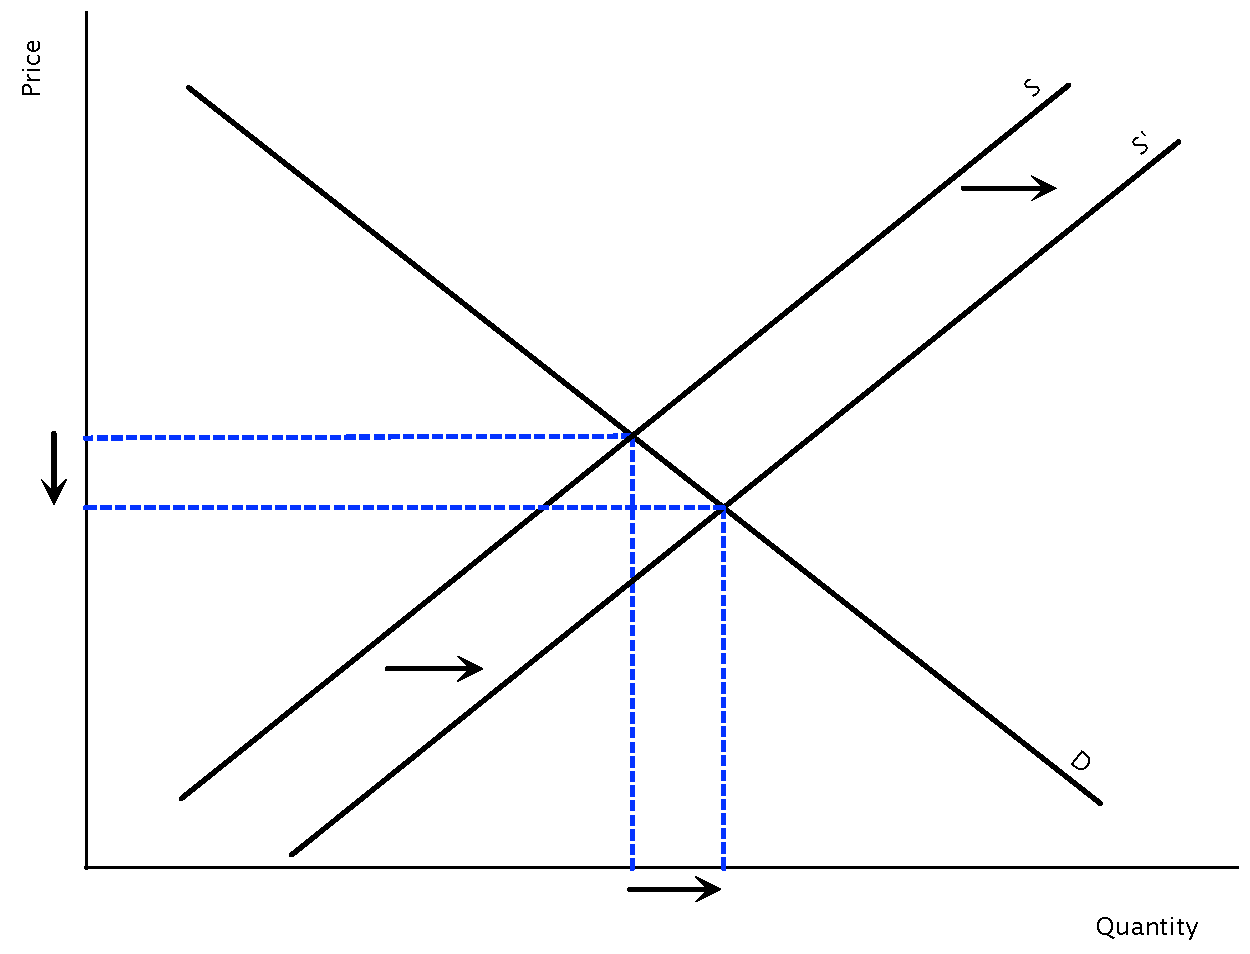
\includegraphics[scale=.25]{plot16.pdf}
					\caption{Effect \#1}
				\end{subfigure}%
				\begin{subfigure}{.5\textwidth}
					\centering
					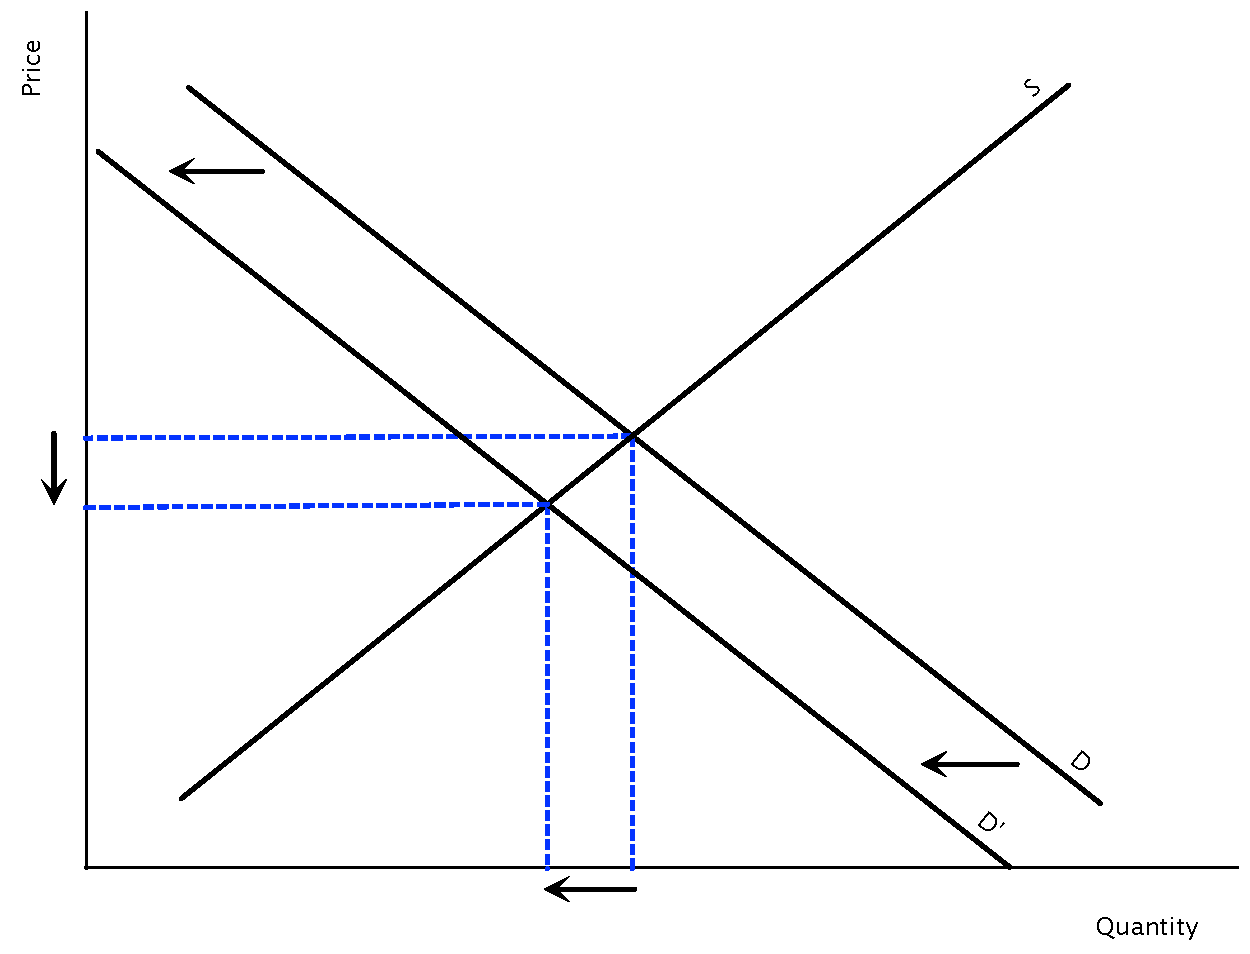
\includegraphics[scale=.25]{plot17.pdf}
					\caption{Effect \#2}
				\end{subfigure}
			\end{figure}
			
	\end{enumerate}
	\end{exmp}
	
	\subsection{Consumer Surplus}
	
	\defn{Willingness to pay:} \ddp{The maximum amount that a buyer will pay for a good/service.\\}
	
	\defn{Consumer surplus:} \ddp{A measure of how well-off a buyer is due to the purchase of a good/service. Calculated as $CS = WTP - P.$ \\}
	
	Consumer surplus is used to measure the well-being of consumers. In particular, it measures the benefit buyers receive from a good \textit{as the buyers themselves perceive it}.
	\\
	
	\begin{exmp} 
		Table \ref{mookie} shows the willingness to pay of Kristina, Josh, Andrea, and Jane for one of Al's Mookie burgers (specifically, the first one they consume). If the market price of these burgers is \$5.50, what is the quantity demanded? How much consumer surplus does each consumer realizes? What is the total consumer surplus in the market as a whole?
	
	\begin{table}[ht]
		\caption{WTP for Mookie Burgers}
		\label{mookie}
		\centering
		\begin{tabular}{  c|c}        
			
			Buyer   & WTP \\
			\hline
			Kristina & \$10.00 \\
			Jane & \$8.50 \\
			Josh & \$5.50 \\
			Andrea & \$4.50 \\
		\end{tabular}
	\end{table} 
	\end{exmp}
	\ddp{$Q_D = 3$. Surplus/person: KV: \$4.50, Jane: \$3, Josh: \$0, Andrea: \$0. Andrea does not buy the burger since $P>WTP$. Total CS = \$7.50.\\}
	
	The demand curve derived from this looks as follows:

\begin{figure}[H]
	\centering
	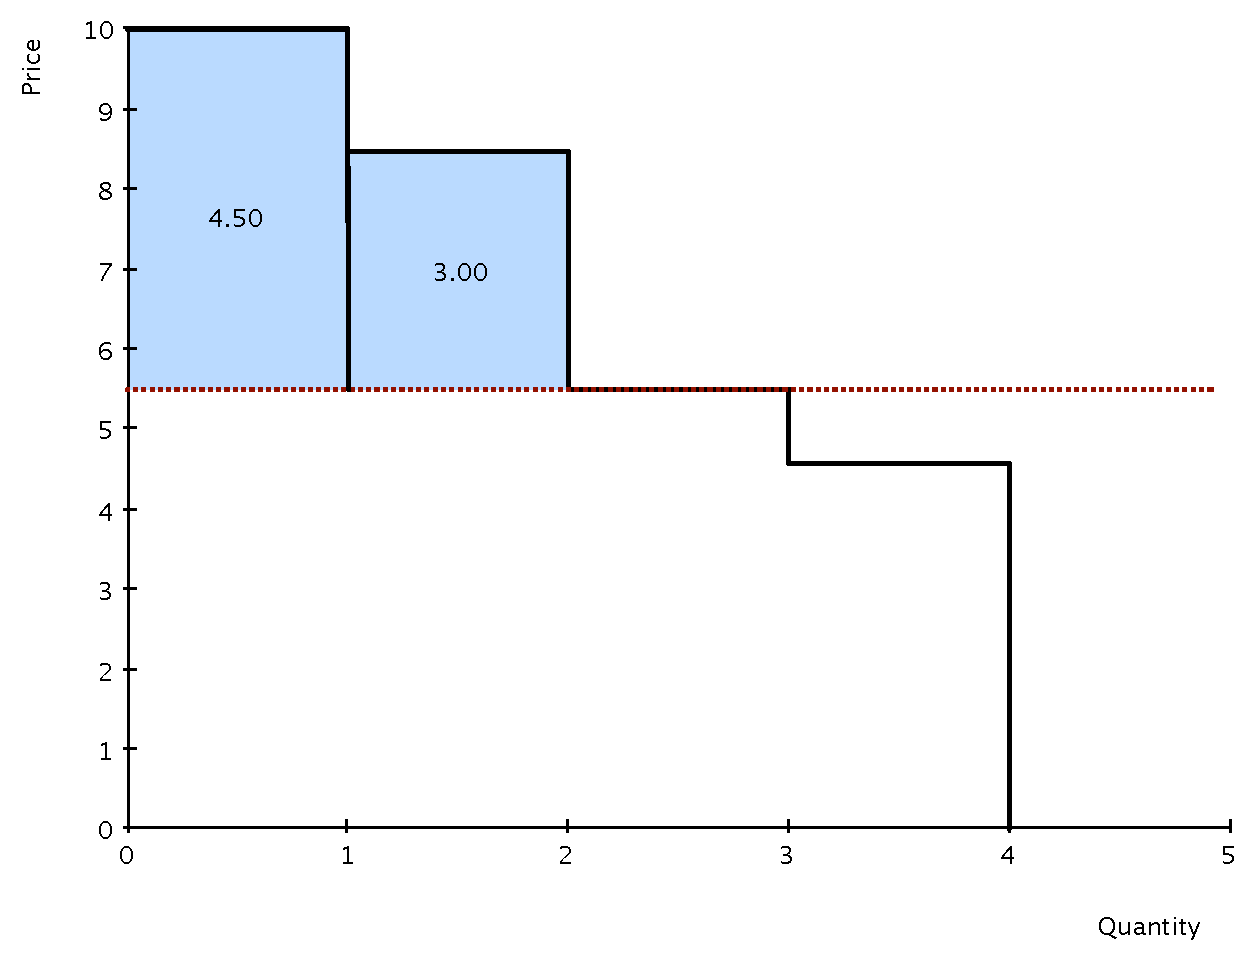
\includegraphics[scale=.35]{plot18.pdf}
	\caption{Demand for Mookie Burgers}
\end{figure}

	Notice that at any quantity, the demand curve shows the willingness to pay of the \textit{marginal buyer}. Thus, we can represent consumer surplus as \dd{the area between demand and the price}.
	\\
	
	If there were enough people and the good was divisible, the steps would get smaller and smaller to eventually form a line (our usual demand curve).
	
	
	\begin{exmp} Consider the demand curve for used economics textbooks for our class. If the market price was \$40, what would be the consumer surplus? What if it was \$30?
	\end{exmp}
	
	\ddp{At \$40, CS = $(1/2)(20)(6) = 60$. At \$30, CS=$(1/2)(30)(9) = 135$.}

\begin{figure}[H]
	\centering
	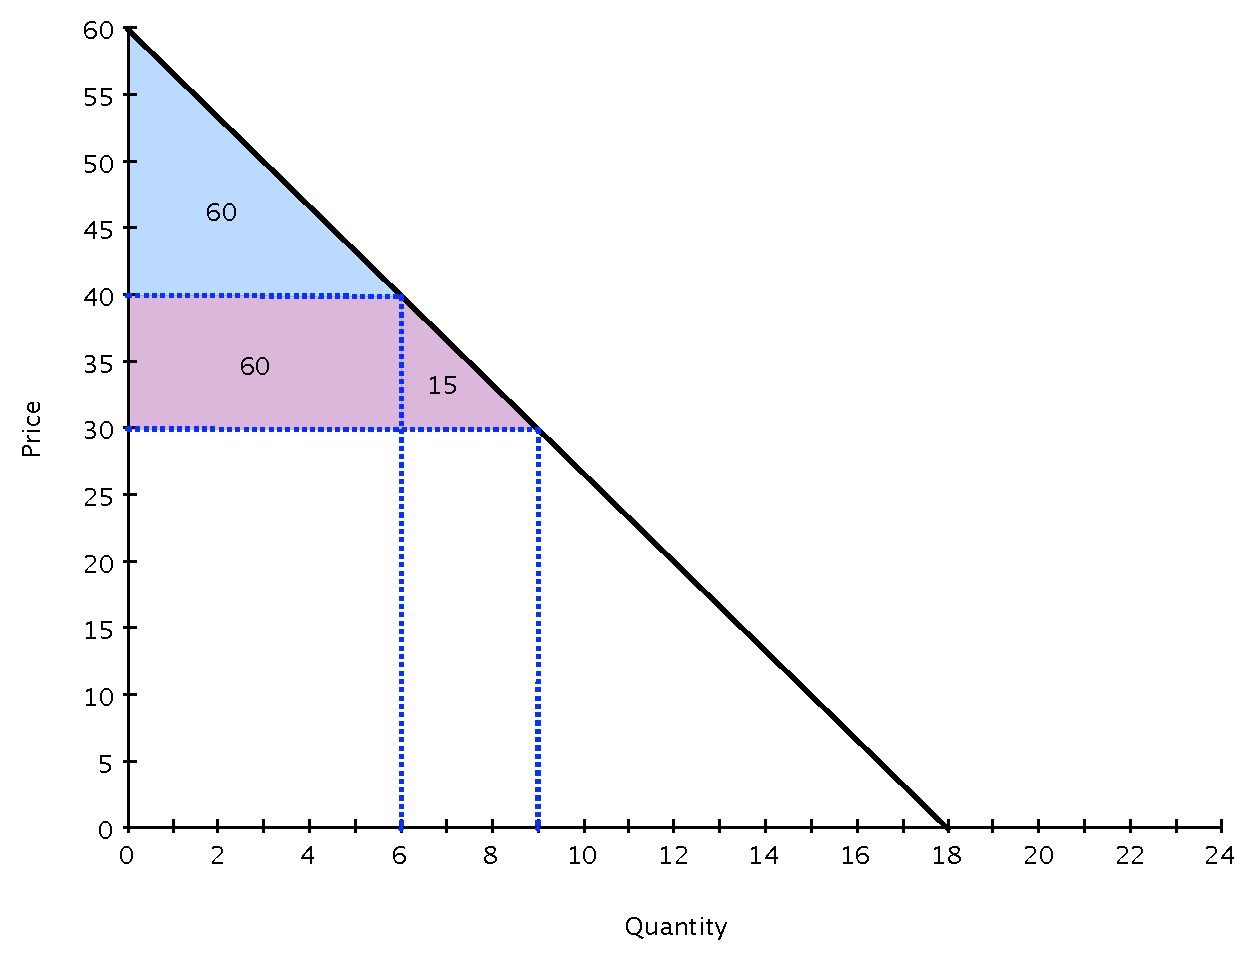
\includegraphics[scale=.35]{plot19.pdf}
	\caption{CS in the Market for Textbooks}
\end{figure}

	Notice that when prices decrease, consumer surplus \dd{increases}. This is due to two reasons: 
	\begin{enumerate}
		\setlength{\itemsep}{15pt}
		\item \ddp{The decrease in prices increases CS for individuals who were already purchasing the good (in Example 4.3, CS to old buyers increased by \$60).}
		\item \ddp{New buyers enter the market due to the lower price and realize CS (in Example 4.3, CS to new buyers is \$15).}
	\end{enumerate}
	
	\subsection{Producer Surplus}
	
	\defn{Cost:} \ddp{The value of everything a seller must give up to produce a good/service.\\}

	
	\defn{Producer Surplus:} \ddp{A measure of well-being for producers who sell a good/service. Calculated as $PS = P - SC$.\\}

	
	\begin{exmp} 
		
		Consider the market for homes. There are four builders in this market, each of which can build a house with the costs shown in Table \ref{tab4}. 
	
	\begin{table}[ht]
		\caption{Cost of Building}
		\label{tab4}
		\centering
		\begin{tabular}{ c|c}        
			
			Seller   & Cost \\
			\hline
			Ace's Builders & \$100,000 \\
			Three Brothers & \$50,000 \\
			ATP & \$200,000 \\
			Craig's Housing & \$300,000 \\
		\end{tabular}
	\end{table} 
	\end{exmp}
	
	Consider what the supply curve would look like under this cost structure. If the market price for houses is \$150,000, what is the quantity supplied and producer surplus in this market? If the price were \$250,000?
		\ddp{\\ At P = 150k, $Q_S = 2$, PS = (150K - 50K) + (150K - 100K) = 150K. \\
			At P = 250K, $Q_S = 3$, PS = (250K - 50K) + (250K - 100K) + (250K - 200K) = 400K.}
		
	\begin{figure}[H]
		\centering
		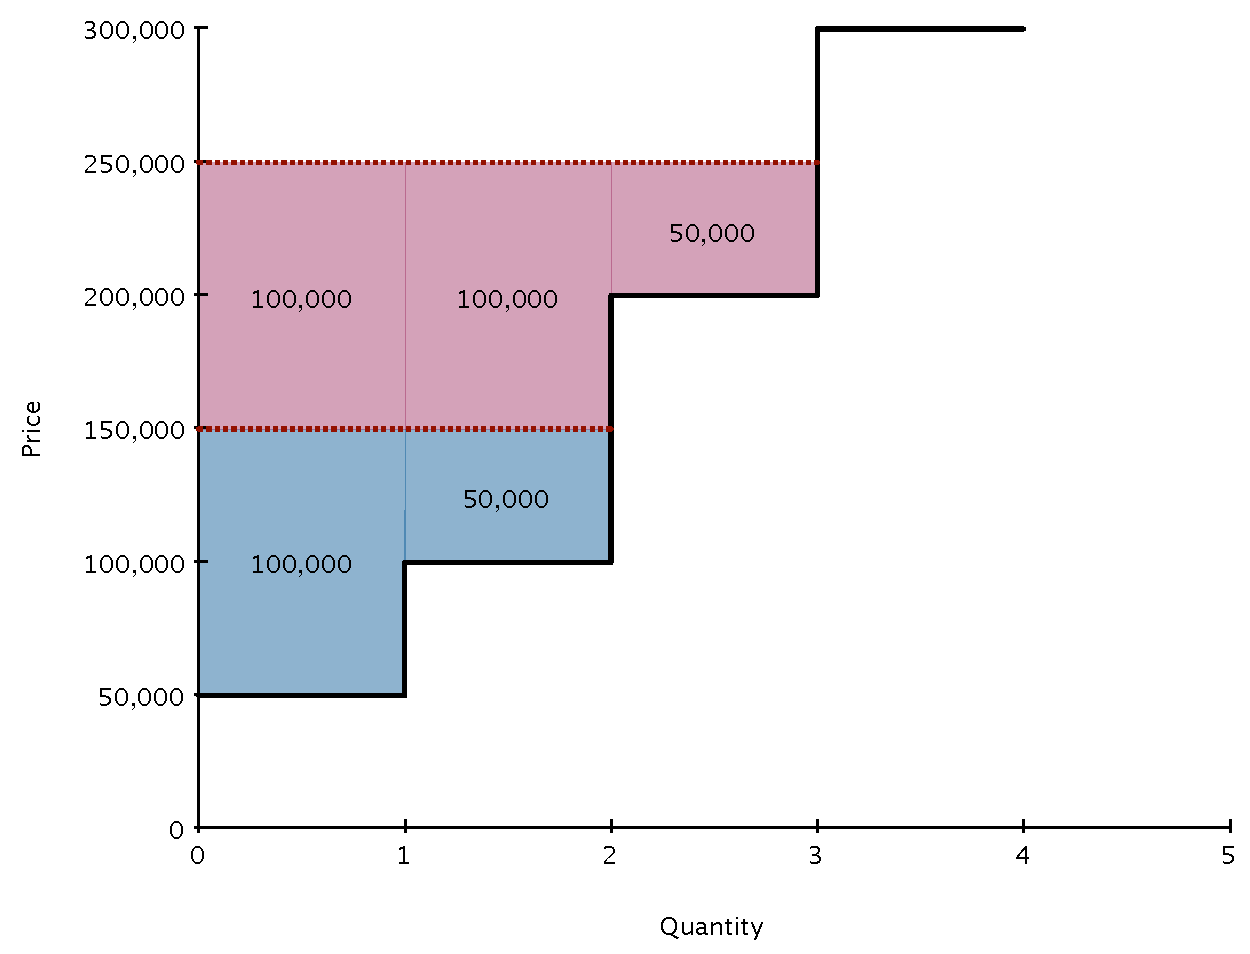
\includegraphics[scale=.40]{plot20.pdf}
		\caption{Supply of Homes}
	\end{figure}
	
	At any quantity, the price given by the supply curve shows the cost of the \textit{marginal seller}. Thus, we can represent producer surplus as \dd{the area b/w the price and the supply curve}.
	\\
	
	Notice that when prices increase, producer surplus \dd{increases}.
	
	\subsection{Efficiency}
	
	\defn{Total Surplus:} \ddp{A measure of the economic well-being of a society. Calculated as $TS = CS + PS = (WTP - P) + (P - SC) = WTP - SC$. Simply the value to buyers minus the cost to sellers. Other actors may realize surplus from markets, even if they don't participate. We will study how that affects surplus later.}

		\begin{exmp} 
			
			Table \ref{blahblah} shows the willingness to pay and seller costs of four buyers and sellers in the market for white Vans. Assume each seller has one pair of shoes to sell and each buyer only wants to buy one pair.
			\begin{table}[ht]
				\caption{Market for White Vans}
				\label{blahblah}
				\centering
				\begin{tabular}{ c|c}        
					
					WTP   & Seller Cost \\
					\hline
					\$45 & \$20 \\
					\$35 & \$40 \\
					\$60 & \$35 \\
					\$40 & \$45 \\
				\end{tabular}
			\end{table}
			
		\begin{enumerate}
	\item	What is the quantity demanded and quantity supplied if the price of vans is \$20? Is this higher or lower than the equilibrium market price? 
		\ddp{\\\\  Buyers with $WTP \ge P$ buy vans. Sellers with $SC \le P$ sell vans. $Q_D$ = 4, $Q_S$ = 1. The market is at a shortage, so $\$20<P^*$.} 
	\blank{}
	\item	What is the quantity demanded and quantity supplied if the price of vans is \$50? Is this higher or lower than the equilibrium market price?
		\ddp{\\\\ Buyers with $WTP \ge P$ buy vans. Sellers with $SC \le P$ sell vans. $Q_D$ = 1, $Q_S$ = 4. The market is at a surplus, so $\$50>P^*$.} 
	\blank{}	
	\item	What is the equilibrium price and quantity in this market? What is the value of total surplus?
		\ddp{\\\\ Order WTP in descending order and SC in ascending order. Market equilibrium at the price where WTP = SC. $P^* = \$40$, $Q^* = 3$.
			\\
			\\
			$TS = WTP - SC = (60 - 20) + (45 - 35) + (40 - 40) = \$50$.}
	\blank{}
\end{enumerate}	
\blank{}	
		\end{exmp}

	
	Consider a market at its equilibrium of supply and demand. Is this equilibrium allocation of resources efficient? 
	
	\begin{figure}[H]
		\centering
		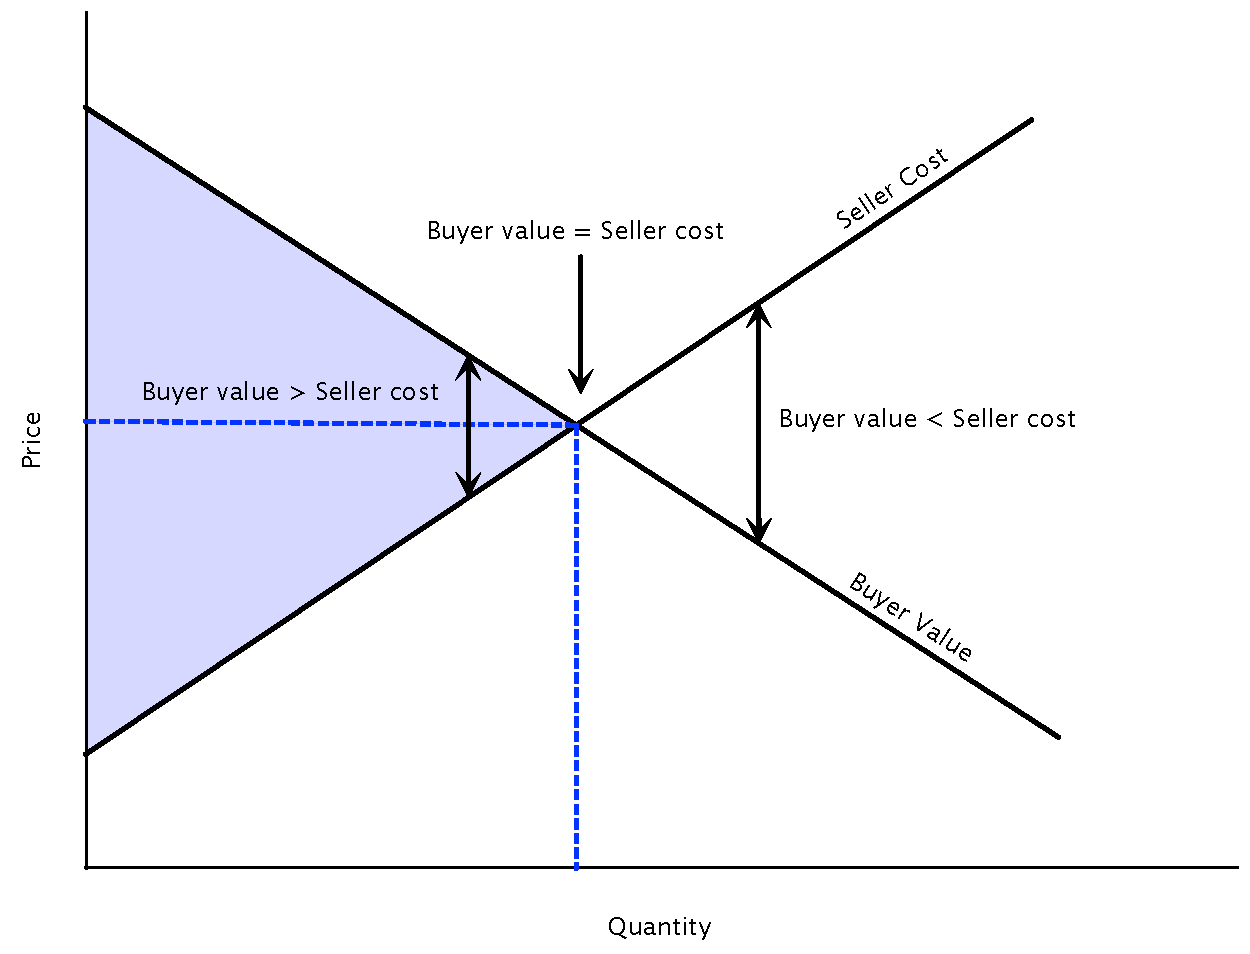
\includegraphics[scale=.35]{plot21.pdf}
		\caption{Total Surplus at Equilibrium}
	\end{figure}
	
	
	
	Insights: 
	\begin{enumerate}
		\item Free markets allocate the supply of goods to the buyers who value them most.
		\item Free markets allocate the demand for goods to the sellers who can produce them at the lowest cost.
		\item Free markets produce the quantity of goods that maximizes the sum of consumer and producer surplus.
	\end{enumerate}
	
	
	If the quantity of goods exchanged was less than the market quantity, we would have \\
	\dd{unrealized gains from trade}.
	\\
	
	\ddp{These are transactions for which $WTP>SC$, so $TS$ would increase if these occurred.\\}

	
	If the quantity of goods exchanged was greater than the market quantity, we would have \\	
	\dd{inefficient transactions}.
	\\
	
	\ddp{These are transactions for which $WTP<SC$, so $TS$ would decrease if these occurred.\\}		

	\textbf{In a perfectly competitive market, the market outcome is efficient.}
	
\newpage
	
	\section{Elasticity and Its Applications}
	
	\defn{Elasticity:} \ddp{A measure of the responsiveness of quantity demanded or quantity supplied to a change in one of its determinants.}
	
	\begin{exmp} 
		Suppose you are looking at the demand for donuts. The price of donuts increases. How much does the quantity demanded decrease?
		
			\begin{figure}[H]
				\centering
				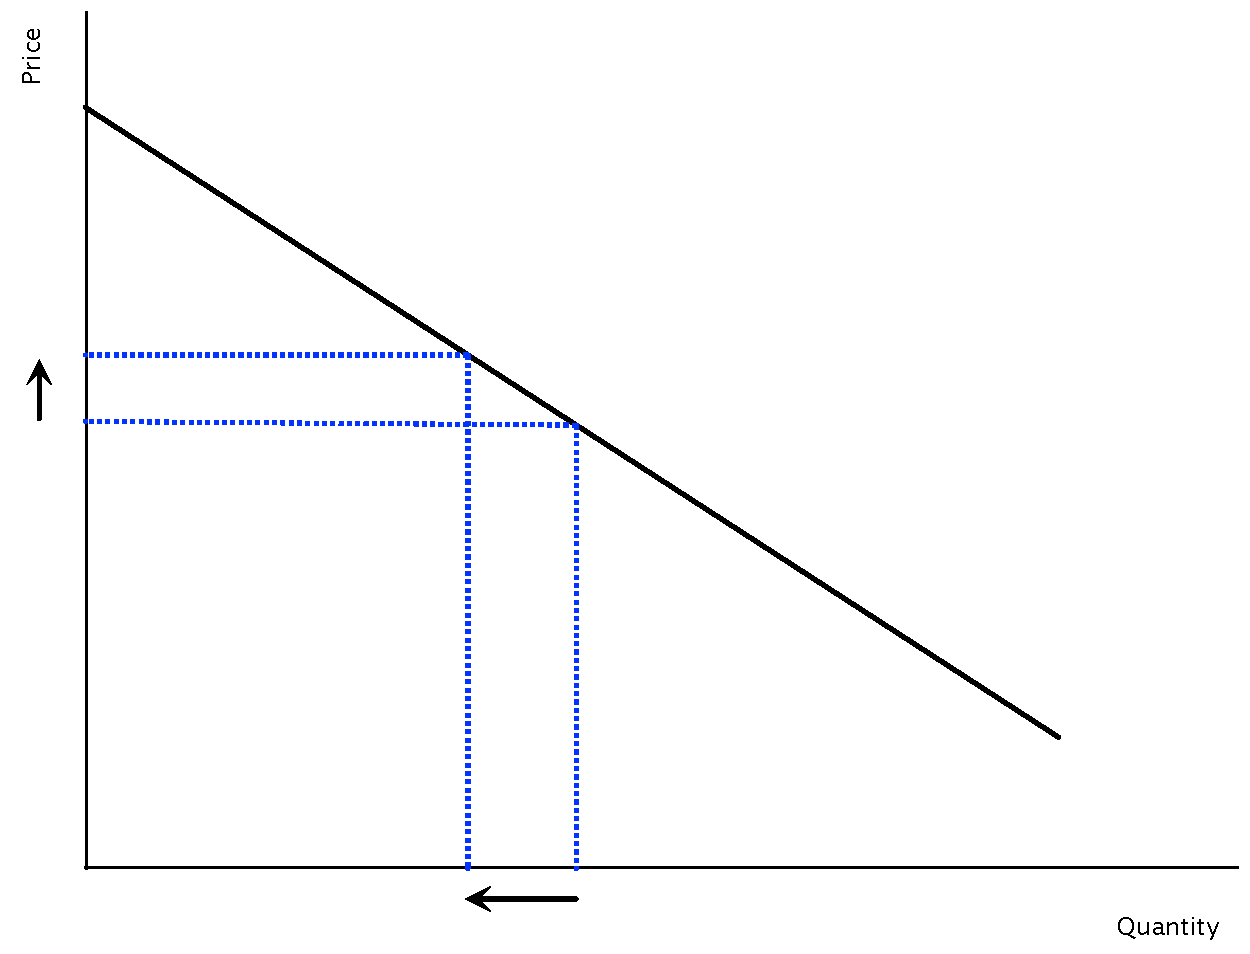
\includegraphics[scale=.40]{plot22.pdf}
				\caption{Market for Donuts}
			\end{figure}
		
	\end{exmp}

	\subsection{The Elasticity of Demand}
	
	\defn{Price Elasticity of Demand:} \ddp{A measure of how much the quantity demanded of a good responds to a change in the price of that good.}
	
		\subsubsection*{Calculating the Price Elasticity of Demand}
		
		
		The price elasticity of demand is measured as the percentage change in quantity demanded divided by the percentage change in price:
		
		\begin{equation*}
		\mathcal{E}_d^p = \frac{\%\Delta Q_d}{\%\Delta P}
		\end{equation*}
		
		
		\begin{exmp} 
			If a 10\% increase in the price of oil leads to a 5\% decrease in the quantity demanded of oil, what is the price elasticity of demand for oil (in absolute terms)?
		\end{exmp}
		\ddp{$\mathcal{E} = |-5\%/10\%| = .5$. This says that the change in $Q_D$ is proportionately half as large as the change in price.}
		\vspace{1em}
		
		The common convention is to report price elasticities of demand in absolute terms. Thus, a larger price elasticity implies a \dd{greater} responsiveness of quantity demanded to changes in price.
		
		\subsubsection*{The Midpoint Method}
		
		
		Typically, percent changes are calculated using what's called the initial value approach:
		
		\begin{equation*}
		\%\Delta X = \ddp{$\frac{X_1 - X_0}{X_0} \times 100\%$}
		\end{equation*}
		
		\begin{exmp} 
			Suppose at a price of \$2, the quantity demanded for pizza is 15. At a price of \$4, the quantity demanded is 10. What is the price elasticity of demand between these points?
		\end{exmp}
		\blank{}
		\blank{}
		\ddp{\\1. $\%\Delta Q_D = \frac{10-15}{15} \times 100\% = -33.3\%$.
			$\%\Delta P = \frac{4-2}{2} \times 100\% = 100\%$. $\Rightarrow |\mathcal{E}| = 33.3/100 = .333$. \\ \\
			2. $\%\Delta Q_D = \frac{15-10}{10} \times 100\% = 50\%$.
			$\%\Delta P = \frac{2-4}{4} \times 100\% = -50\%$. $\Rightarrow |\mathcal{E}| = 50/50 = 1$. \\}
		
		The midpoint method is a way to calculate percentage changes such that the percentage change from $A$ to $B$ is the same as the percentage change from $B$ to $A$. It is calculated as follows:
		
		
		\begin{equation*}
		\%\Delta X = \ddp{$\frac{X_1 - X_0}{\Big(\frac{X_0+X_1}{2}\Big)} \times 100\%$}
		\end{equation*}
		
		
		\begin{exmp}
			Calculate the price elasticity of demand for pizza using the midpoint method.
		\end{exmp}
		\ddp{$\%\Delta Q_D = \frac{15 - 10}{(15+10)/2} \times 100\% = 40\%$. $\%\Delta P = \frac{2-4}{(2+4)/2} \times 100\% = -66.7\% \Rightarrow |\mathcal{E}| = 40/66.7 = .60$.\\}
		\blank{}

	\subsubsection*{Factors that Influence $\mathcal{E}_d^p$:}
	
	
	\begin{enumerate}
		\setlength{\itemsep}{15pt}
		\item Availability of substitutes 
		\ddp{\\More close substitutes allows individuals to switch to other goods, so quantity demanded is more responsive to changes in prices. More close substitutes  $\Rightarrow$ more elastic demand.}
		\item Necessities vs. Luxuries
		\ddp{\\ Necessities have more inelastic demand. Luxuries have more elastic demand.}
		\item Definition of the market
		\ddp{\\Broadly defined markets have less elastic demand (e.g., easier to move from Wonka chocolate to other brands vs moving from chocolate to another type of candy.)}
		\item Time Horizon
		\ddp{\\Demand becomes more elastic over a longer time horizon as consumers are more able to adjust their purchasing habits.}
	\end{enumerate}
	

	
	
	\defn{Inelastic Demand:} \ddp{Demand is considered to be inelastic when $\mathcal{E} < 1$. Not very responsive to changes in price.\\}
	
	
	\defn{Elastic Demand:} \ddp{Elastic when $\mathcal{E} > 1$. Very responsive to changes in price.\\}
	
	
	\defn{Unit Elastic Demand:} \ddp{$\mathcal{E} = 1$. The change in $Q_D$ is proportional to the change in $P$.\\}
	
		
		\begin{exmp}
			
			Which of the following products would tend to have inelastic demand? Why?
			\begin{enumerate}[(a)]
				{\setlength\itemindent{25pt} \item Luxury sedans} \ddp{Luxury}
				{\setlength\itemindent{25pt} \item Candy} \ddp{Lots of substitutes}
				{\setlength\itemindent{25pt} \item Crude oil} \ddp{Not many substitutes}
				{\setlength\itemindent{25pt} \item Black Angus T-bone steak} \ddp{Narrowly defined market.}
			\end{enumerate}
		\end{exmp}
		\ddp{Option (c).}

	\subsubsection*{Characterizing Points Along a Demand Curve}
	Even though the slope of a linear demand curve is constant, the elasticity is not. Linear demand curves have the characteristic that at points with a low price and high quantity, the demand curve is \dd{inelastic}. At points with a high price and low quantity, the demand curve is \dd{elastic}.

		\begin{figure}[H]
			\centering
			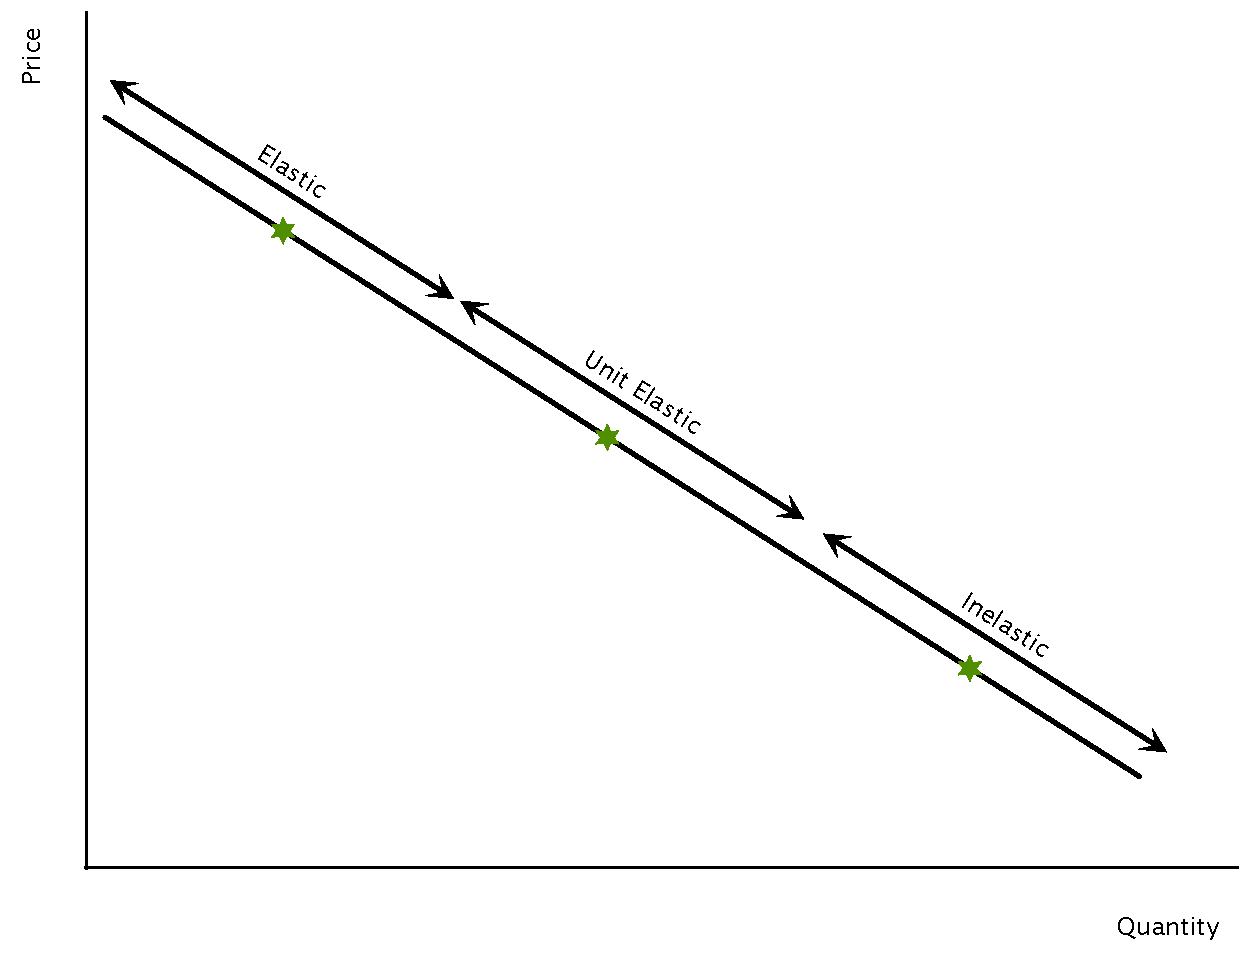
\includegraphics[scale=.42]{plot23.pdf}
			\caption{Points along a Demand Curve}
		\end{figure}

	
	\subsubsection*{Comparing Demand Curves}
	
	
	Because the price elasticity of demand measures how much quantity demanded responds to changes in price, it is closely related to the slope of the demand curve. Rearranging the equation for the price elasticity of demand, we have that
	
	\begin{equation*}
	|\mathcal{E}_d^p|= \ddp{$\Big(\frac{P_0 + P_1}{Q_0 + Q_1}\Big) \times \Big|\frac{1}{m}\Big|$.}
	\end{equation*}

	Thus, a flatter demand curve is \dd{relatively elastic} compared to a steeper curve. 
	\\
	
	Conversely, a steeper demand curve is  \dd{relatively inelastic} compared to a flatter curve.
	\\
	
	\begin{exmp}
		Refer to Figure \ref{fig1}. The price elasticity of demand in the left panel is \dd{greater} than the price elasticity of demand in the right panel.
	
	\begin{figure}[H]
		\centering
		\caption{Comparing Demand Elasticities}
		\label{fig1}
		\begin{subfigure}{.5\textwidth}
			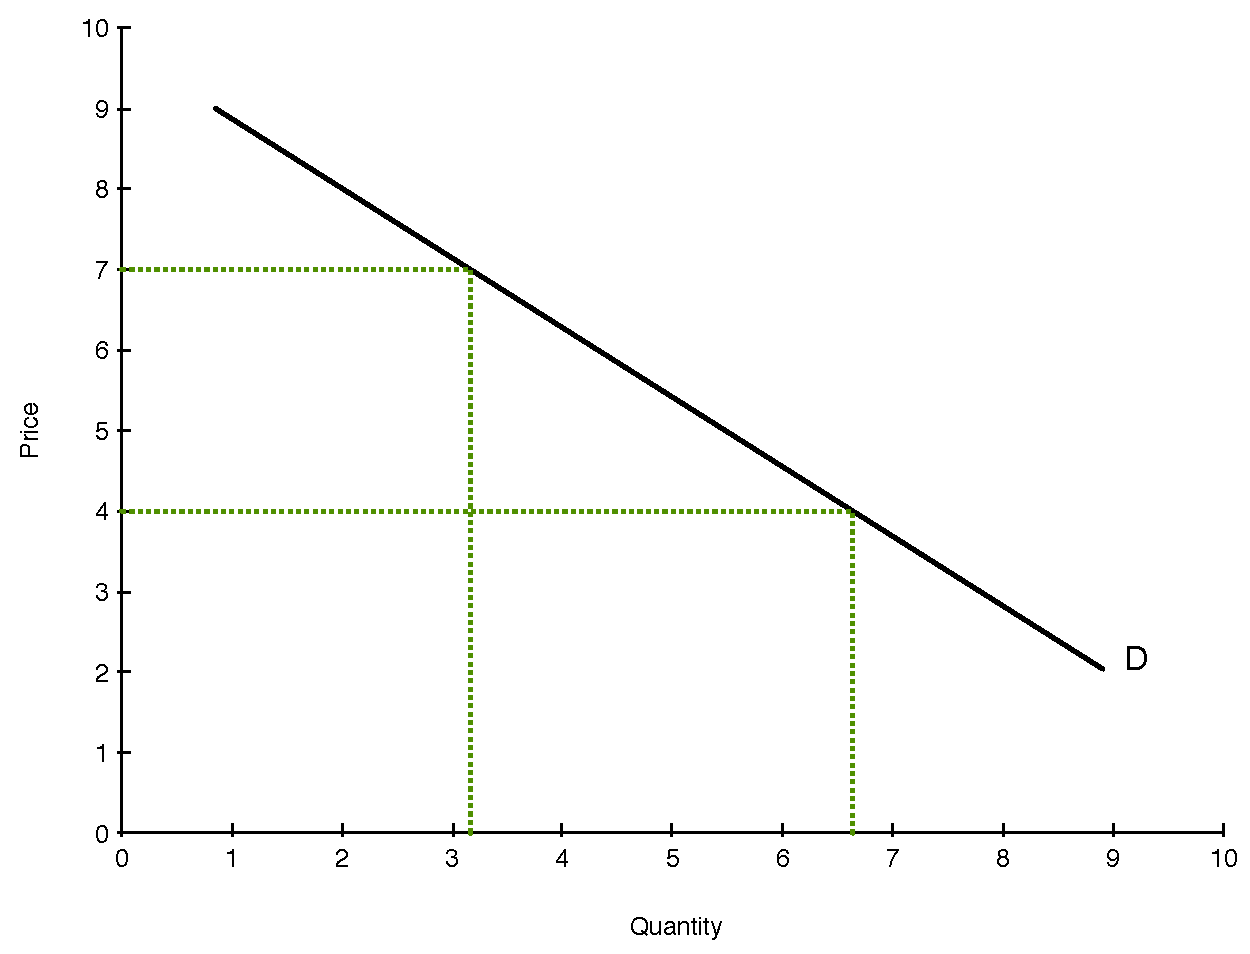
\includegraphics[scale=.3]{notes04_plot1.pdf}
			\caption{Relatively Elastic\\ Demand Curve}
		\end{subfigure}%
		\begin{subfigure}{.5\textwidth}
			\centering
			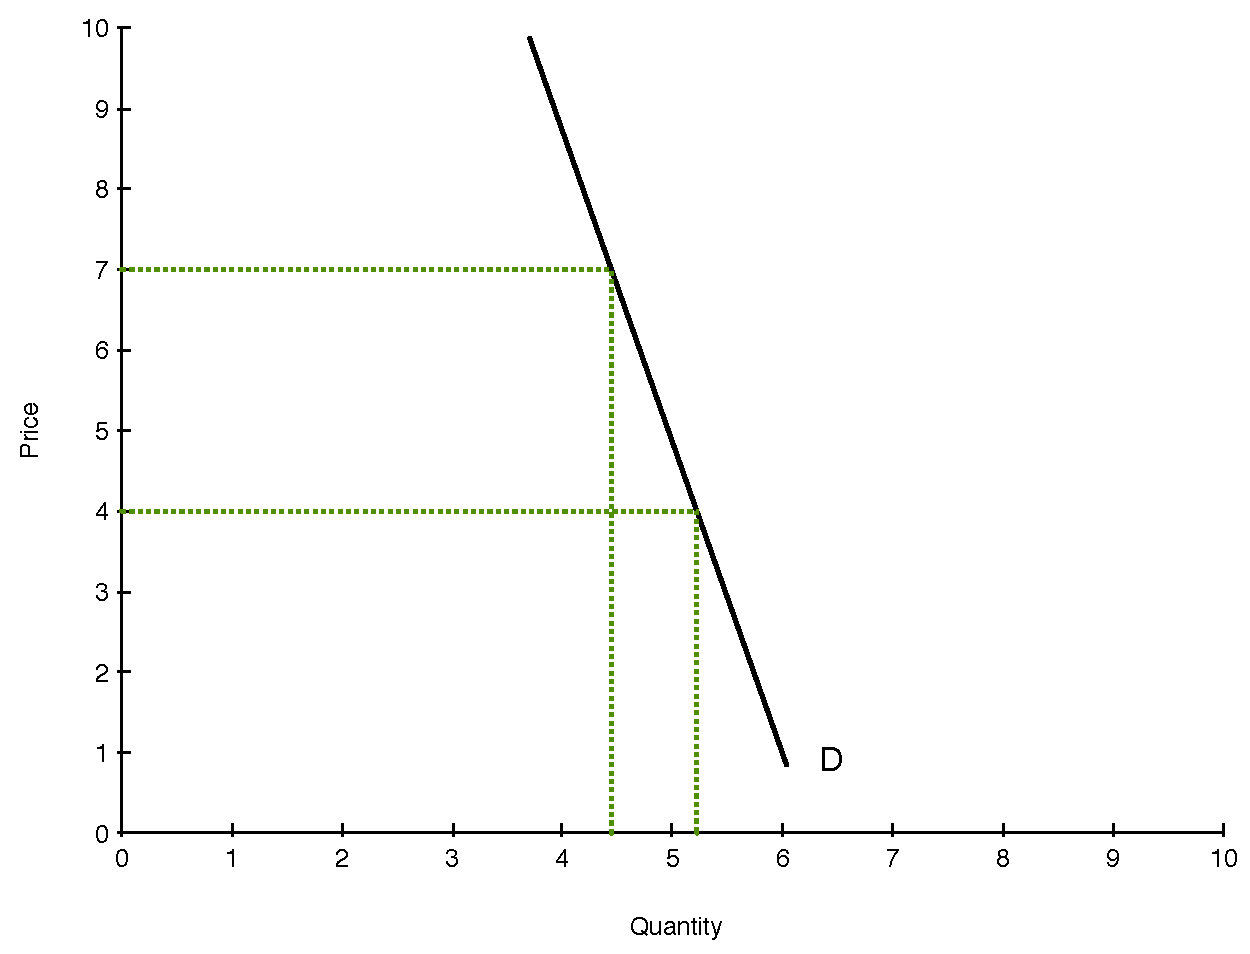
\includegraphics[scale=.3]{notes04_plot2.pdf}
			\caption{Relatively Inelastic \\ Demand Curve}
		\end{subfigure}
	\end{figure}
\end{exmp}

		
			\begin{figure}[H]
				\centering
				\caption{Extreme Cases}
				\begin{subfigure}{.5\textwidth}
					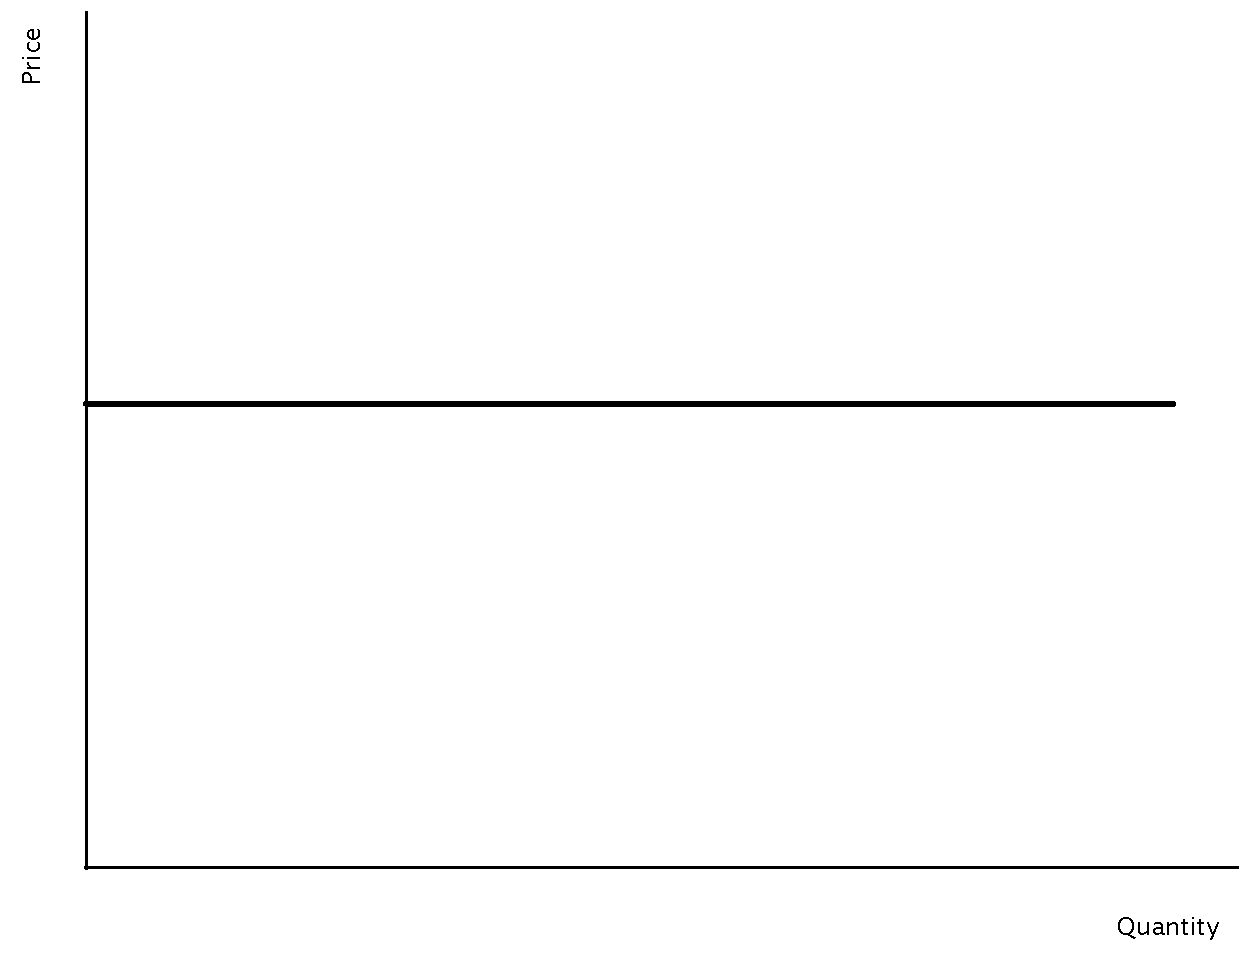
\includegraphics[scale=.3]{plot24.pdf}
					\caption{Perfectly Elastic Demand}
				\end{subfigure}%
				\begin{subfigure}{.5\textwidth}
					\centering
					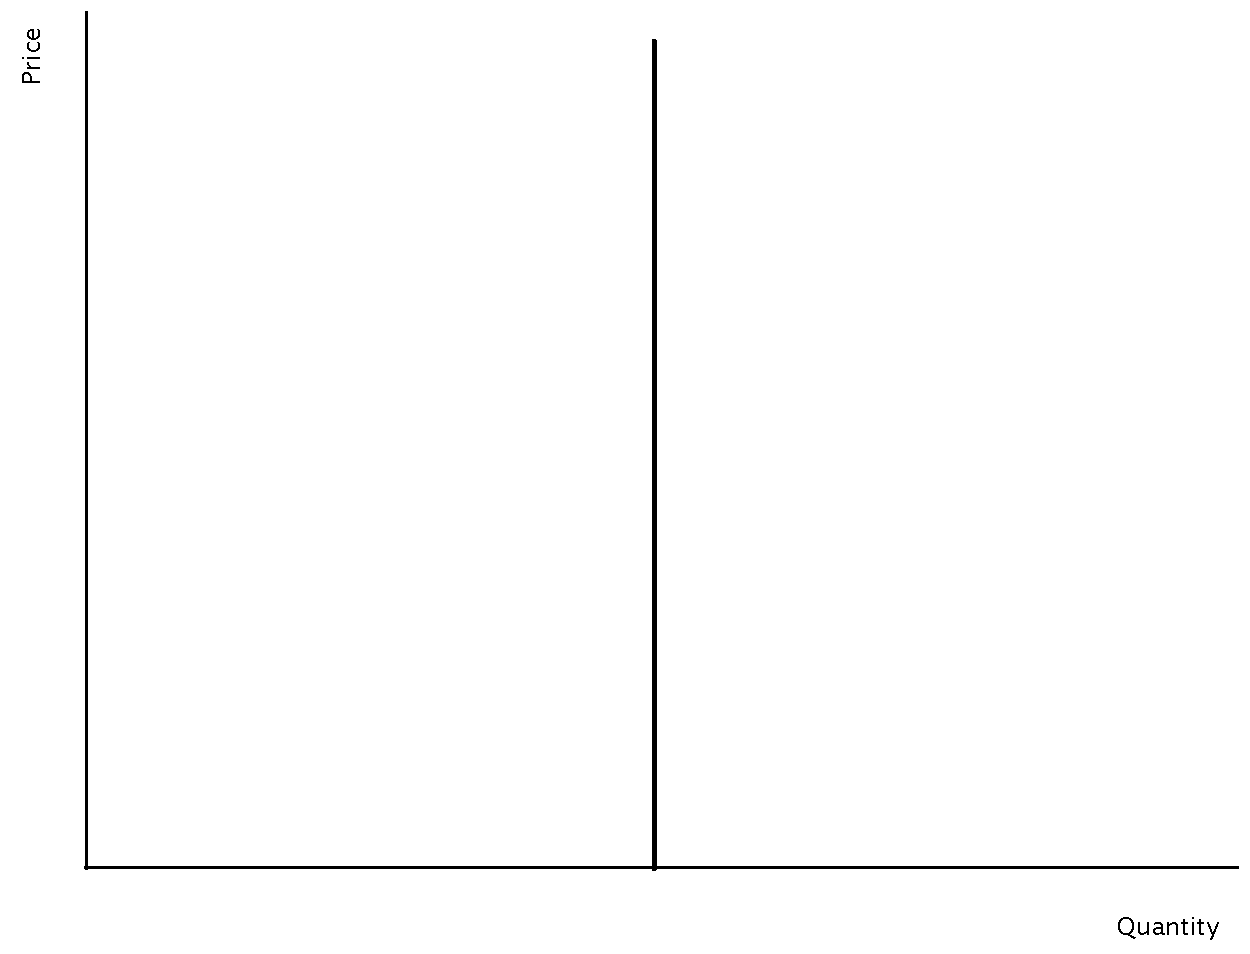
\includegraphics[scale=.3]{plot25.pdf}
					\caption{Perfectly Inelastic Demand}
				\end{subfigure}
			\end{figure}

	
	\begin{exmp} 
		Megan goes to her favorite coffee shop every morning and always buys one large black coffee, not matter whether there is a special or not. What is her price elasticity of demand?
	\end{exmp}
	
	\blank{}
	
	\ddp{No matter what the price is, quantity demanded does not change. Her price elasticity of demand is zero and she has a perfectly inelastic demand curve.}
	
	\subsubsection*{Total Revenue and Price Elasticity of Demand}
	
	
	\defn{Total Revenue:} \ddp{The total amount paid by buyers \& received by sellers of a good. $TR = P\times Q$.}

		\begin{figure}[H]
			\centering
			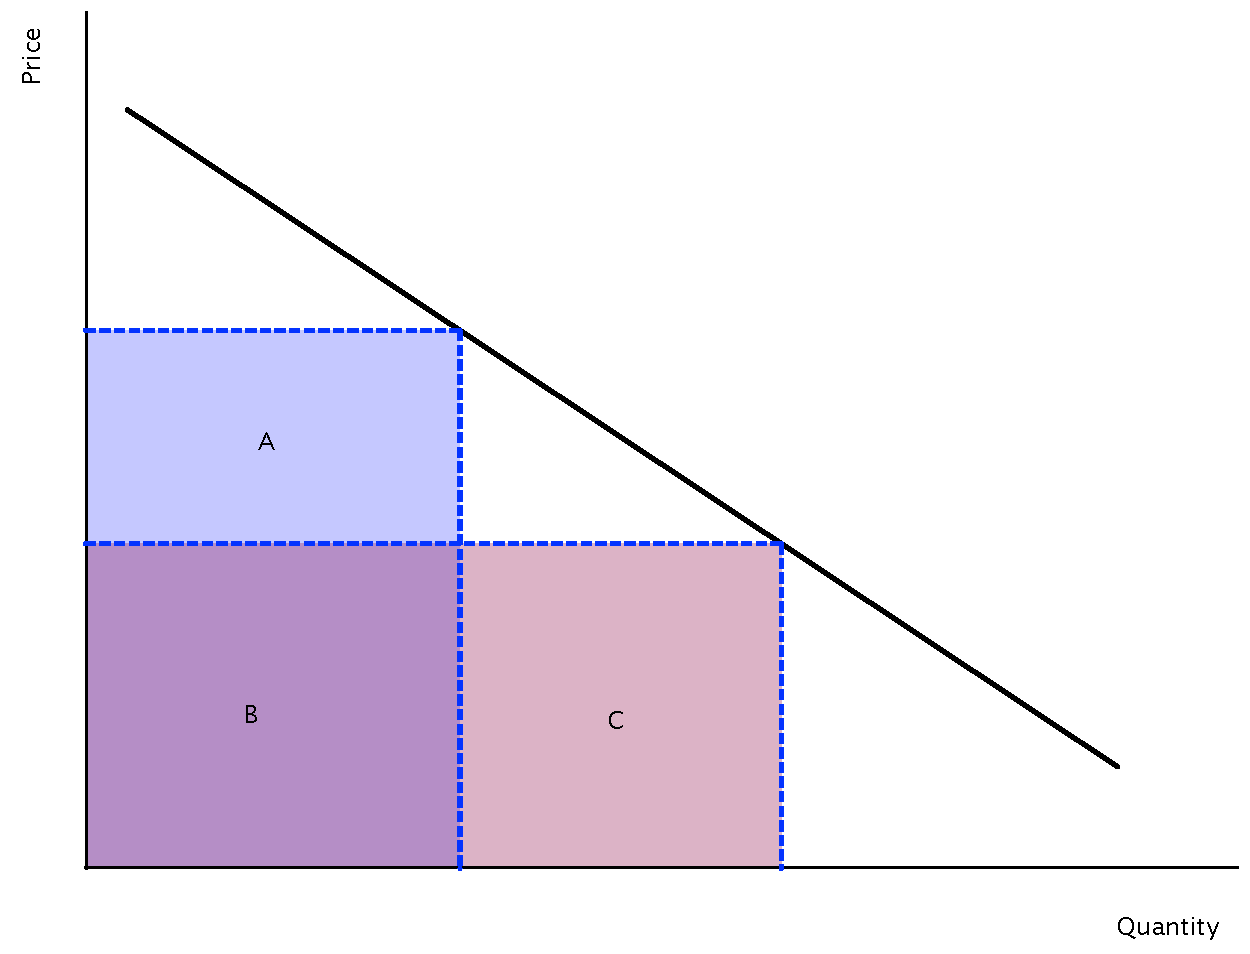
\includegraphics[scale=.38]{plot26.pdf}
			\caption{Total Revenue and Elasticity}
		\end{figure}
	

	As prices change, the change in total revenue depends on the elasticity of demand.
	\\
	
	We can write the percentage change in total revenue as \dd{$\%\Delta TR \approx \% \Delta P + \%\Delta Q_D$.}
	\\
	
	If demand is inelastic, \dd{$|\% \Delta P| > |\%\Delta Q_D$|}. Thus, if prices rise then total revenue will \dd{increase}.
	\\

	If demand is elastic, \dd{$|\% \Delta P| < |\%\Delta Q_D$|}. Thus, if prices rise then total revenue will \dd{decrease}.
	\\
	
	If demand is unit elastic, \dd{$|\% \Delta P| = |\%\Delta Q_D$|}. Thus, total revenue will \dd{not change} when the price changes.
	
	
		\begin{figure}[H]
			\centering
			\caption{Comparing Demand Elasticities and Total Revenue}
			\begin{subfigure}{.3\textwidth}
				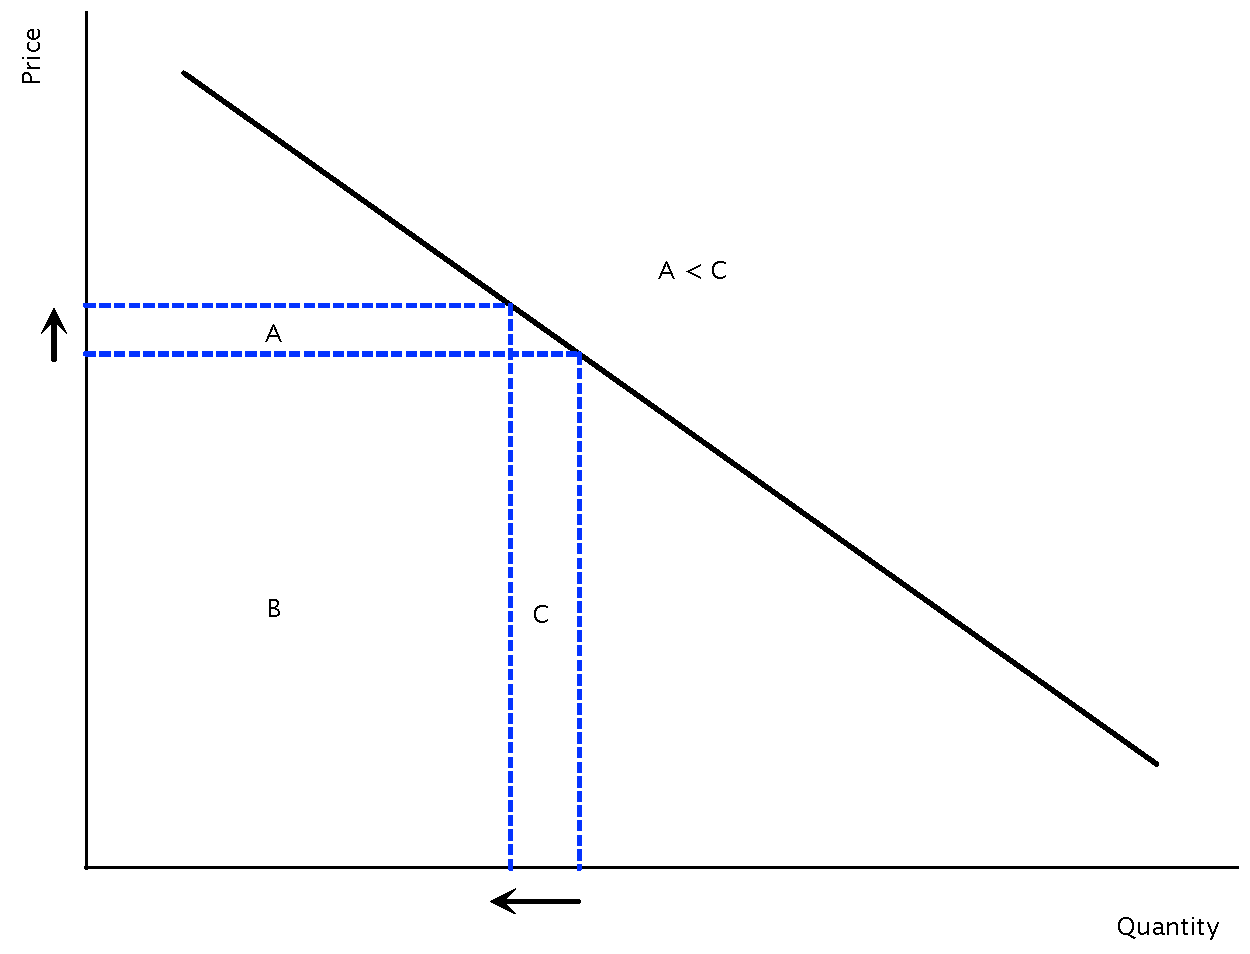
\includegraphics[scale=.3]{plot27.pdf}
				\caption{Elastic Point}
			\end{subfigure}%
			\begin{subfigure}{.3\textwidth}
				\centering
				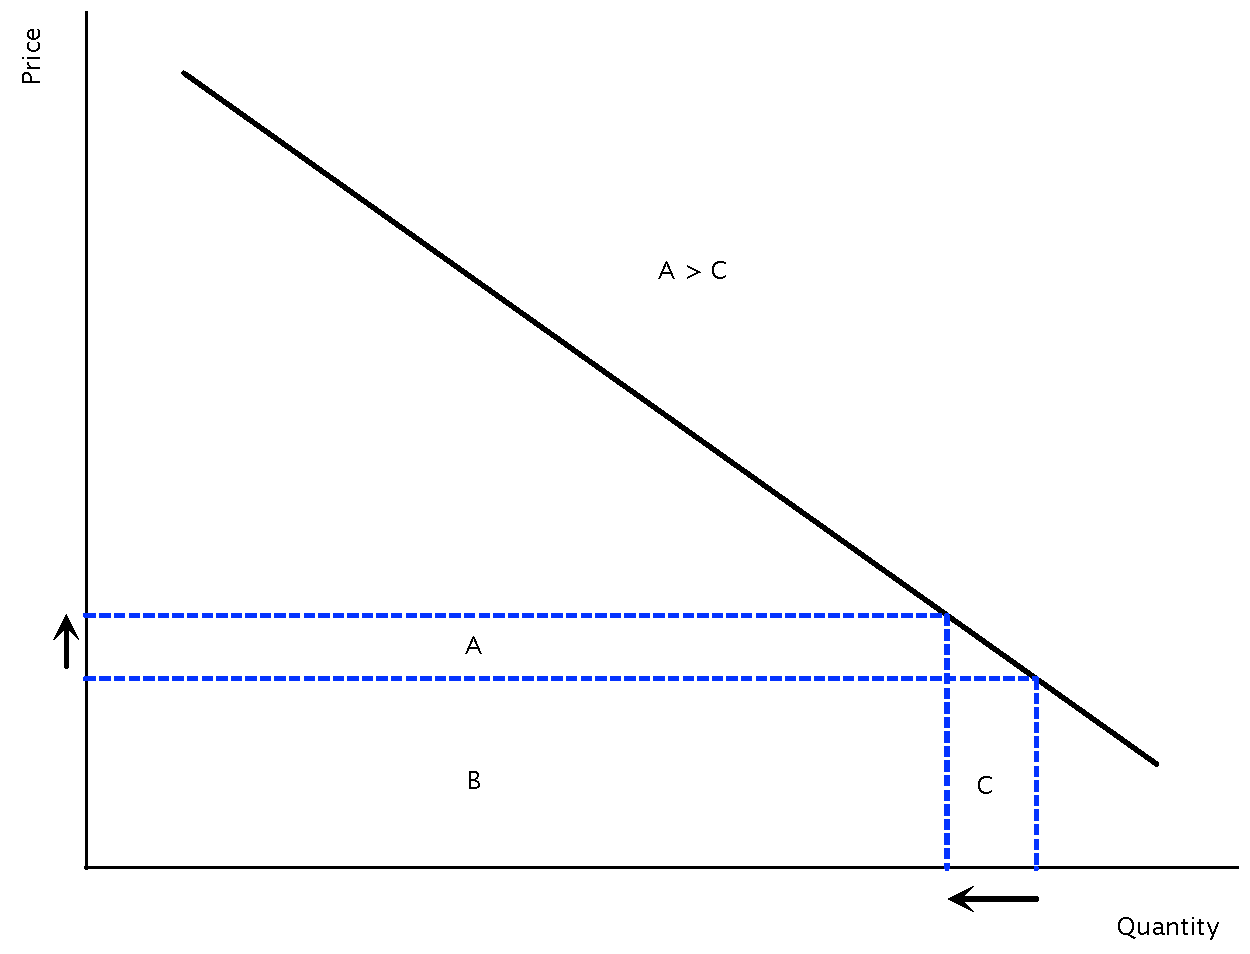
\includegraphics[scale=.3]{plot29.pdf}
				\caption{Inelastic Point}
			\end{subfigure}
			\begin{subfigure}{.3\textwidth}
				\centering
				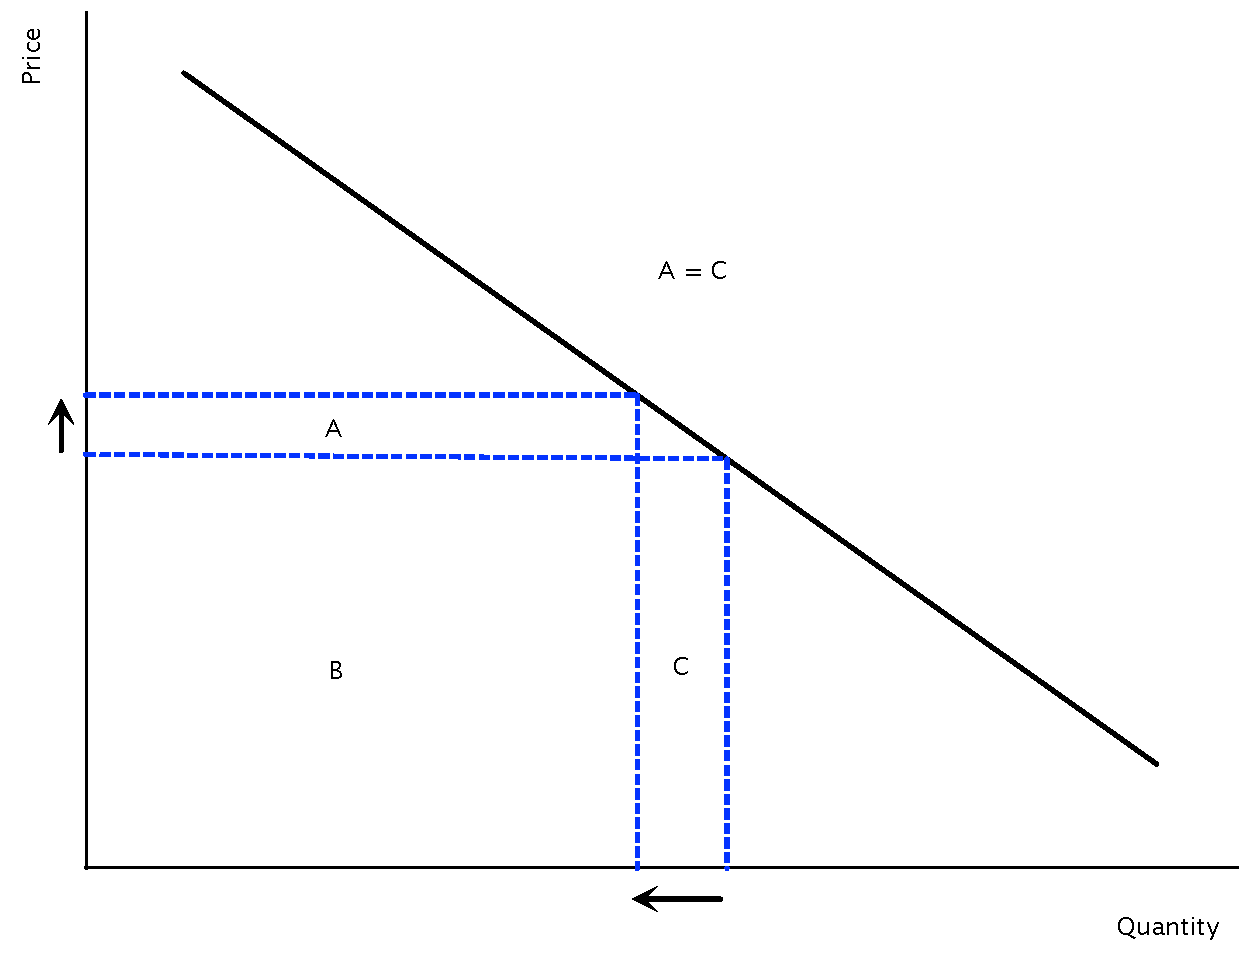
\includegraphics[scale=.3]{plot28.pdf}
				\caption{Unit Elastic Point}
			\end{subfigure}
		\end{figure}
	
	\begin{exmp}
		You decide to work as a private tutor to fund your trip and want to raise as much money as possible. Should you increase or decrease the price you charge? Explain.
	\end{exmp} 
	\blank{}
	\ddp{Depends on elasticity of demand. If elastic, lower prices. If inelastic, raise prices.}

	
	\begin{exmp} 
		The local pizza restaurant makes such great bread sticks that consumers do not respond much at all to a change in the price. If the owner is only interested in increasing revenue, he should
	
	\begin{enumerate}[(a)]
		{\setlength\itemindent{25pt} \item lower the price of bread sticks}
		{\setlength\itemindent{25pt} \item leave the price of bread sticks alone}
		{\setlength\itemindent{25pt} \item raise the price of bread sticks}
		{\setlength\itemindent{25pt} \item reduce costs}
	\end{enumerate}	
	\end{exmp}
	
	\ddp{Consumers aren't responsive to price changes, so demand is inelastic. He should increase the price of breadsticks (c).}

	\begin{exmp} 
		
		Assume drug addicts pay for their addictions by stealing so that the higher the total revenue of the illegal drug industry, the higher the amount of theft.
		
		\begin{enumerate}
			\item Suppose the government cracks down on drug suppliers by imposing stiff penalties for those caught dealing drugs. How will this affect the price of illegal drugs?
			
				\begin{figure}[H]
					\centering
					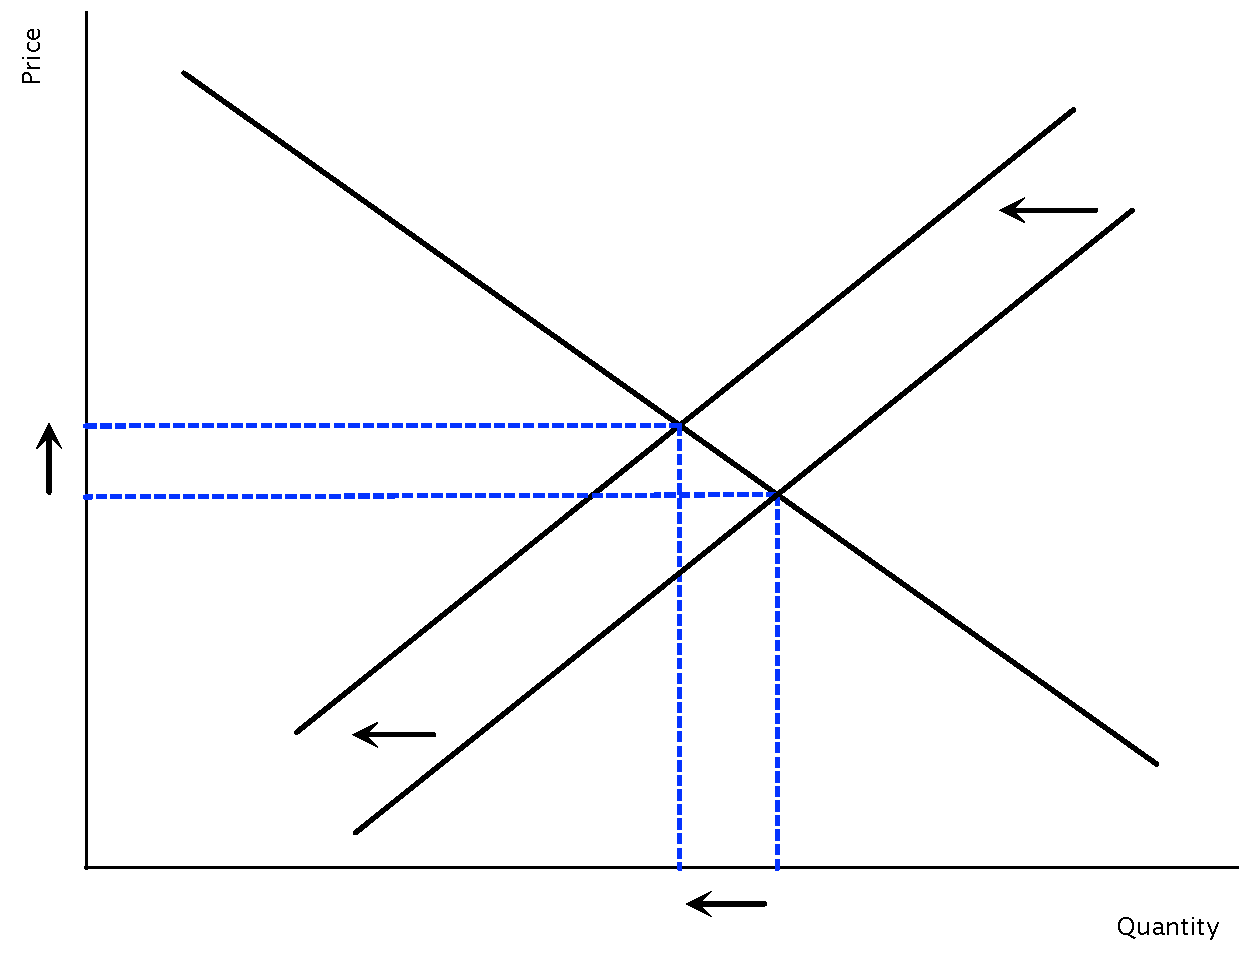
\includegraphics[scale=.35]{plot30.pdf}
					\caption{Example 5.10.1}
				\end{figure}
				
			\ddp{The price of drugs will increase since supply decreases. The change in total revenue depends on the elasticity of demand.}
				
			\item What happens to the amount of stealing if the demand for drugs is elastic? Inelastic?
			
				\begin{figure}[H]
					\centering
					\caption{Example 5.10.2}
					\begin{subfigure}{.5\textwidth}
						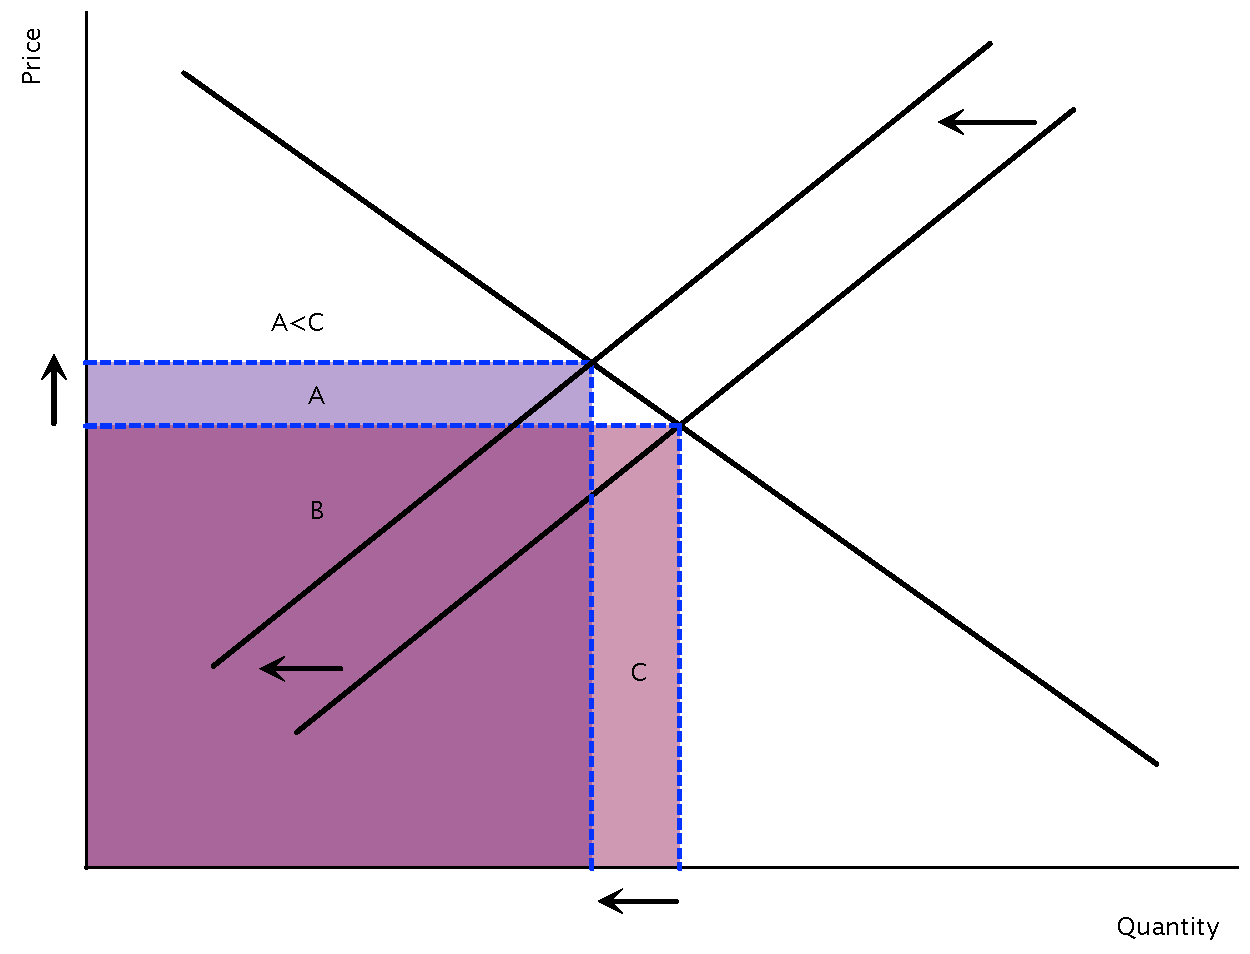
\includegraphics[scale=.3]{plot31.pdf}
						\caption{Elastic Case}
					\end{subfigure}%
					\begin{subfigure}{.5\textwidth}
						\centering
						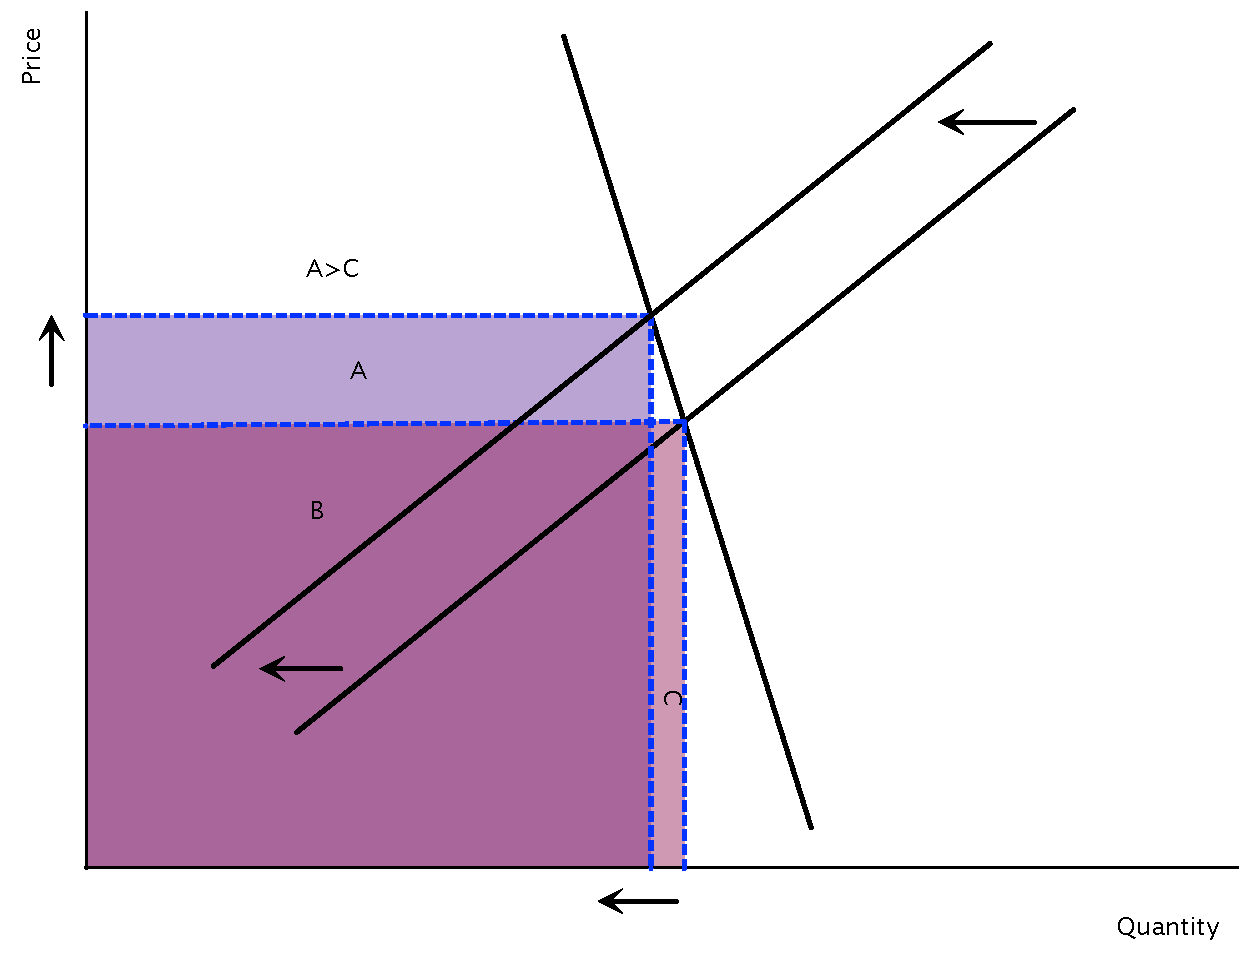
\includegraphics[scale=.3]{plot32.pdf}
						\caption{Inelastic Case}
					\end{subfigure}
				\end{figure}
				
				\ddp{In the elastic case, the amount of stealing will decrease because the decrease in quantity will outweigh the increase in price. In the inelastic case, stealing will increase since the price effect will dominate.}
			
			\item If instead the government pursued a policy of drug education that reduced the demand for drugs, what would be the effect on stealing? 
			
				\begin{figure}[H]
					\centering
					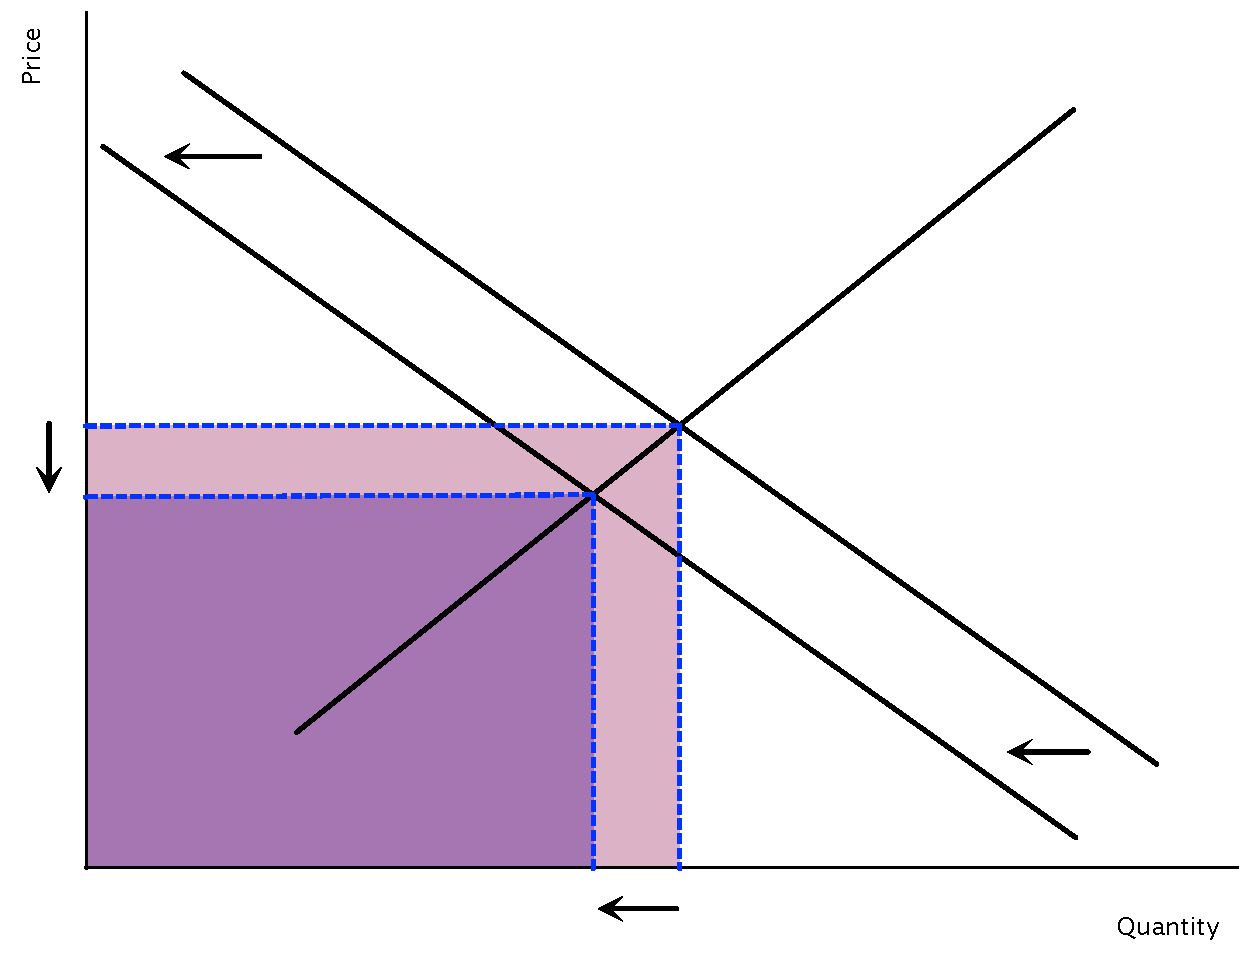
\includegraphics[scale=.40]{plot33.pdf}
					\caption{Drug Education Policy}
				\end{figure}
				
				\ddp{The drug education policy will result in both a lower equilibrium price and quantity, which will reduce the amount of stealing.}
			
		\end{enumerate}
	\end{exmp}
	
	\subsection{Other Demand Elasticities}
	
	\begin{itemize}
		\item \defn{Income elasticity of demand:} \ddp{A measure of how much quantity demanded responds to a change in consumers' income.\\}
		
		$\mathcal{E}_d^I =$ \ddp{$\frac{\% \Delta Q_D}{\% \Delta I}$} 
		\\
		
		If a good is \defn{normal}, a higher (lower) income will increase (decrease) quantity demanded. Thus,  $\mathcal{E}_d^I$ is \dd{positive} for these goods because if \dd{$\%\Delta I\gtrless  0$}, then \dd{$\%\Delta Q_D\gtrless  0$}. 
		\\
		
		If a good is \defn{inferior},  a higher (lower) income will decrease (increase) quantity demanded. Thus, $\mathcal{E}_d^I$ is \dd{negative} for these goods because if \dd{$\%\Delta I\gtrless  0$}, then \dd{$\%\Delta Q_D\lessgtr  0$}. 
		
		\item \defn{Cross-price elasticity of demand:} \ddp{A measure of how much the quantity demanded of one good responds to a change in the price of another good.}
		\\
	
		 $\mathcal{E}_{d_x}^{p_y} =$ \ddp{$\frac{\% \Delta Q_{D_x}}{\% \Delta P_y}$} 
		\\
		
		If the goods are \defn{substitutes}, an increase (decrease) in the price of one good increases (decreases) the quantity demanded of the other. Thus, $\mathcal{E}_{d_x}^{p_y}$ is \dd{positive} because if \dd{$\%\Delta P_y \gtrless  0$}, then \dd{$\%\Delta Q_{D_x}\gtrless 0$}. 
		\\
		
		If the goods are \defn{complements}, an increase (decrease) in the price of one good decreases (increases) the quantity demanded of the other. Thus, $\mathcal{E}_{d_x}^{p_y}$ is \dd{negative} because if  \dd{$\%\Delta P_y\gtrless  0$}, then \dd{$\%\Delta Q_{D_x} \lessgtr  0$}. 
		
	\end{itemize}

	
	Importantly, when computing \textbf{any} elasticities, it must be done keeping \textbf{all} other determinants of quantity demanded constant.
\\
	
\begin{exmp} 
	Figure \ref{fig2} shows that the demand for Converse shoes has increased because average consumer incomes have increased from \$2,000 to \$4,000. What is the income elasticity of demand for Converse shoes?

\begin{figure}[H]
	\centering
	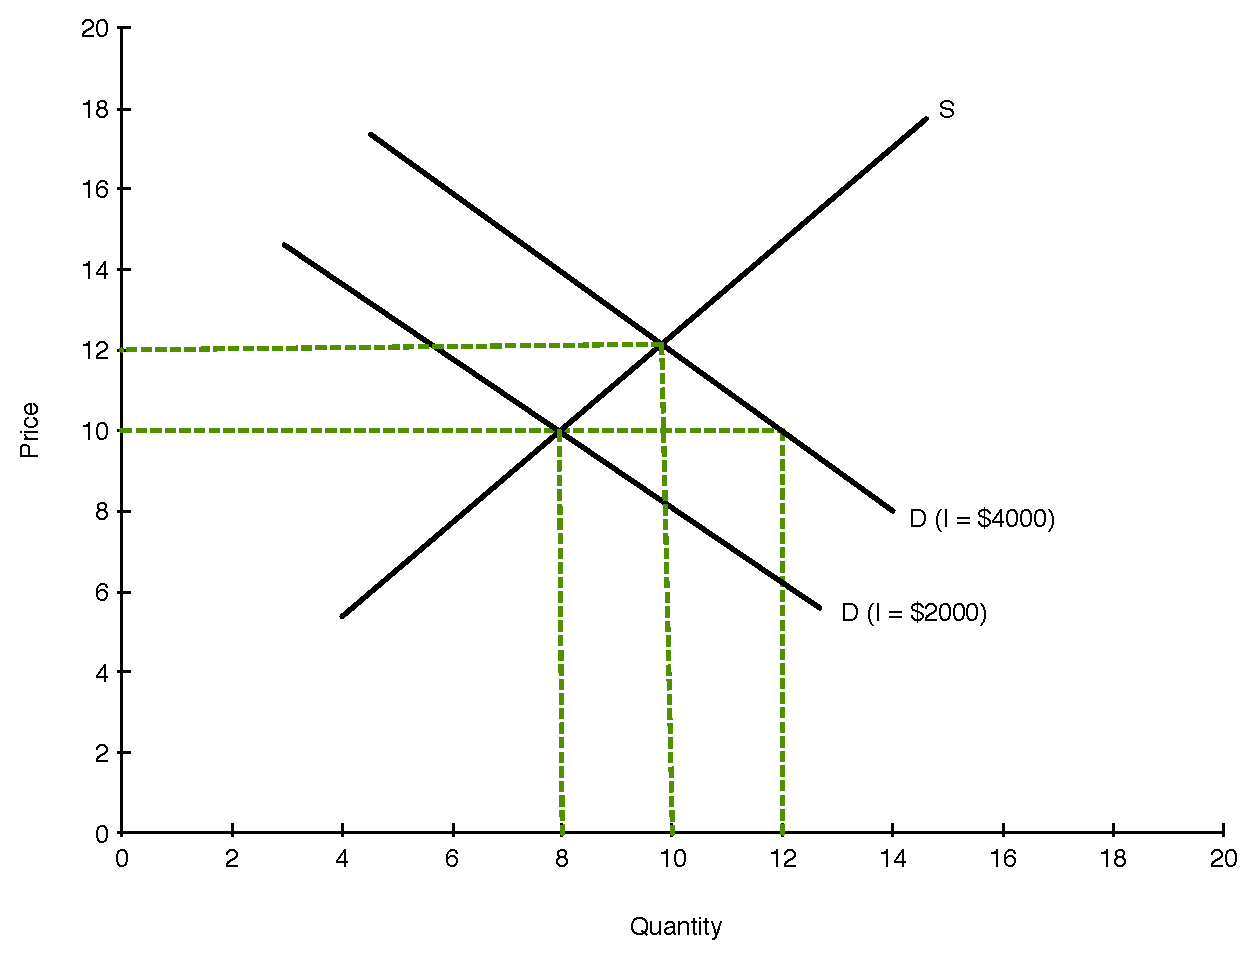
\includegraphics[scale=.33]{hw2_plot1.pdf}
	\caption{Market for Converse Shoes}
	\label{fig2}
\end{figure}
\end{exmp}
\ddp{Hold price constant at $P=\$10$. $Q_0 = 8,$ $Q_1 = 12.$ $\% \Delta Q_D = 12-8/10 = .4.$ $\% \Delta I = 4000-2000/3000 = .67.$ $\mathcal{E}_d^I = .4/.67 = .60.$ This is a normal good since the income elasticity is positive.}
	
	\subsection{The Elasticity of Supply}
	
	\defn{Price Elasticity of Supply:} \ddp{A measure of how much quantity supplied responds to changes in prices of a good.}
	\\
	
	The major determinant of price elasticity of supply we will examine is the time horizon. In the long run, supply is \dd{more elastic}.
	\ddp{\\ \\Firms are able adjust their fixed costs in the long run.}
	

\newpage	
	
	\section{Government Policy}
	
	The focus of this section is to analyze different types of government policies using the tools of supply and demand. Additionally, it will look at the welfare implications of such policies.
	
	\subsection{Price  Ceilings}
	
	\defn{Price ceiling:} \ddp{A legal maximum on the price at which a good can be sold.\\}
	
	Consider two types of price ceilings, one that is above the market price and one that is below:
	
		\begin{figure}[H]
			\centering
			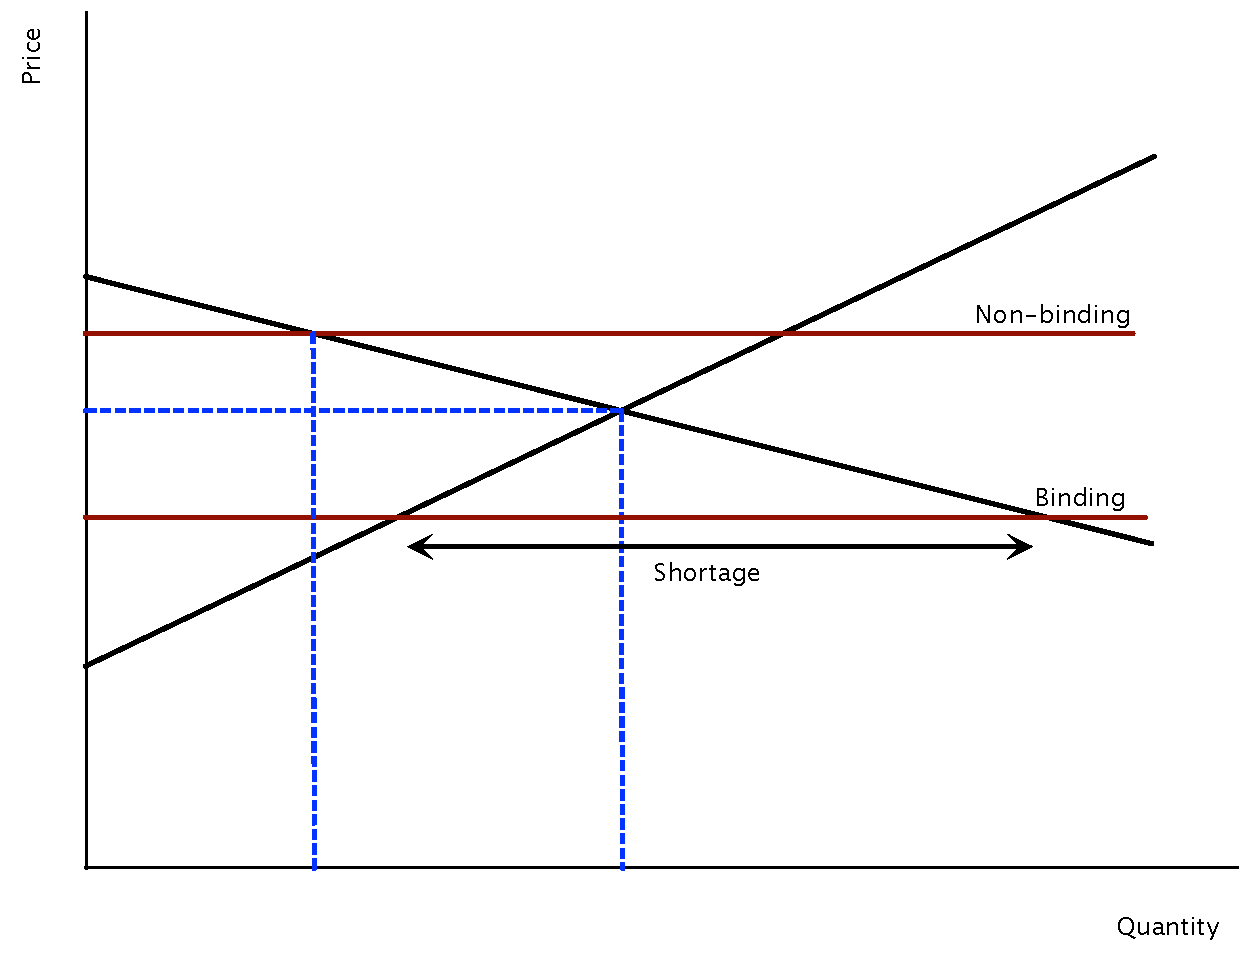
\includegraphics[scale=.40]{plot34.pdf}
			\caption{Price Ceilings}
		\end{figure}
	
	If the government sets a price ceiling above the market price, then the ceiling is \dd{non-binding}.
	\\
	
	If the government sets a price ceiling below the market price, then the ceiling is \dd{binding}.
	\\
	
	Market forces move the economy towards the equilibrium point where $Q_d = Q_s$. In the case of a binding price ceiling, once the price in the market hits the ceiling it cannot increase any further by law. Therefore, if the price ceiling is binding, the market price equals the price ceiling.
	\\
	
	At this price, we have that \dd{$Q_D$} is greater than \dd{$Q_S$}. Thus, there is a \dd{shortage}.
	\\
	
	Due to this shortage, some mechanism for rationing will develop. Two potential ones are
	\begin{enumerate}
		\item \ddp{Long lines}
		\item \ddp{Rationing according to seller bias}
	\end{enumerate}
	

	Both types of rationing mechanisms above are not \dd{efficient}. 
	\begin{enumerate}
		\item \ddp{Long lines waste time}
		\item \ddp{Seller bias: goods do not necessarily go to the buyer that values it most.}
	\end{enumerate}
	
	On the other hand, free markets ration goods with \dd{prices}. This mechanism is both \dd{efficient} and \dd{impartial}.
	
	\subsubsection*{Welfare Considerations}
	
	
	Consider a market before the introduction of a binding price ceiling and afterwards:
	
		\begin{figure}[H]
			\centering
			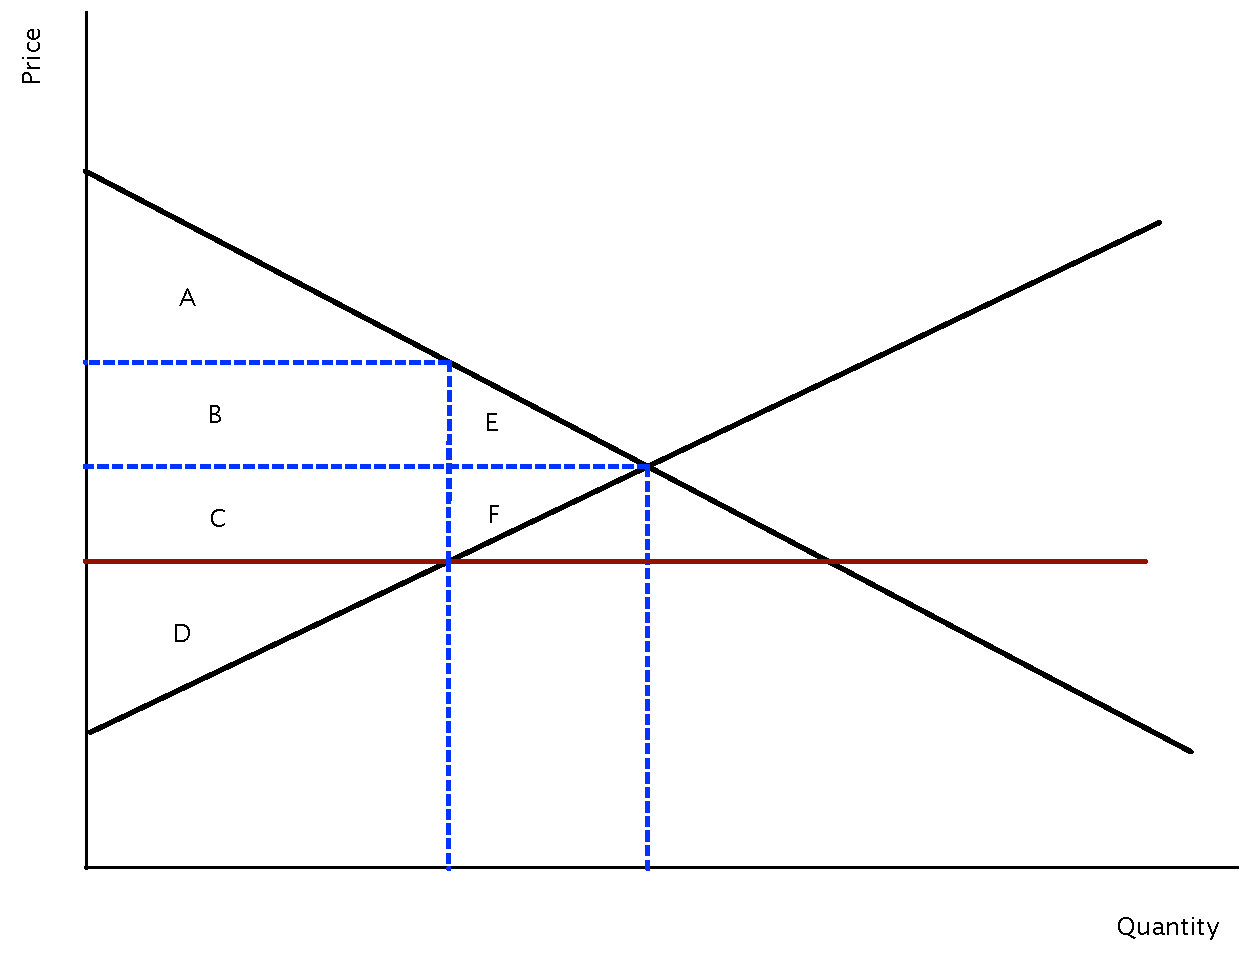
\includegraphics[scale=.40]{plot36.pdf}
			\caption{Price Ceilings and Welfare}
		\end{figure}
		
	
	
	Before the introduction of the ceiling, buyers and sellers were paying and receiving price $P^*$. Thus, 
	\begin{align*}
	\text{CS}_0 &= \ddp{A + B + E}\\
	\text{PS}_0 &= \ddp{C + D + F}\\
	\text{TS}_0 &= \ddp{A + B + C + D + E + F}
	\phantom{\hspace{9cm}}
	\end{align*}
	
	After the price ceiling is introduced, the market price is $P_C$. Buyers and sellers are now paying and receiving \dd{less} than before. Moreover, the number of transactions that are taking place has \dd{decreased}. Now, 
	\begin{align*}
	\text{CS}_1 &= \ddp{A + B + C}\\
	\text{PS}_1 &= \ddp{D}\\
	\text{TS}_1 &= \ddp{A + B + C + D}
	\phantom{\hspace{9cm}}
	\end{align*}
	
	
	This \dd{decrease} in total surplus (the area \dd{E + F}) is referred to as a \dd{deadweight loss}.
	\\
	
	\defn{Deadweight Loss (DWL):} \ddp{The decrease in total surplus that results from a market distortion.}
	
	\subsection{Price Floors}
	
	\defn{Price floor:} \ddp{A legal minimum on the price at which a good can be sold.\\}
	
	Consider two types of price floors, one that is above the market price and one that is below:
	
		\begin{figure}[H]
			\centering
			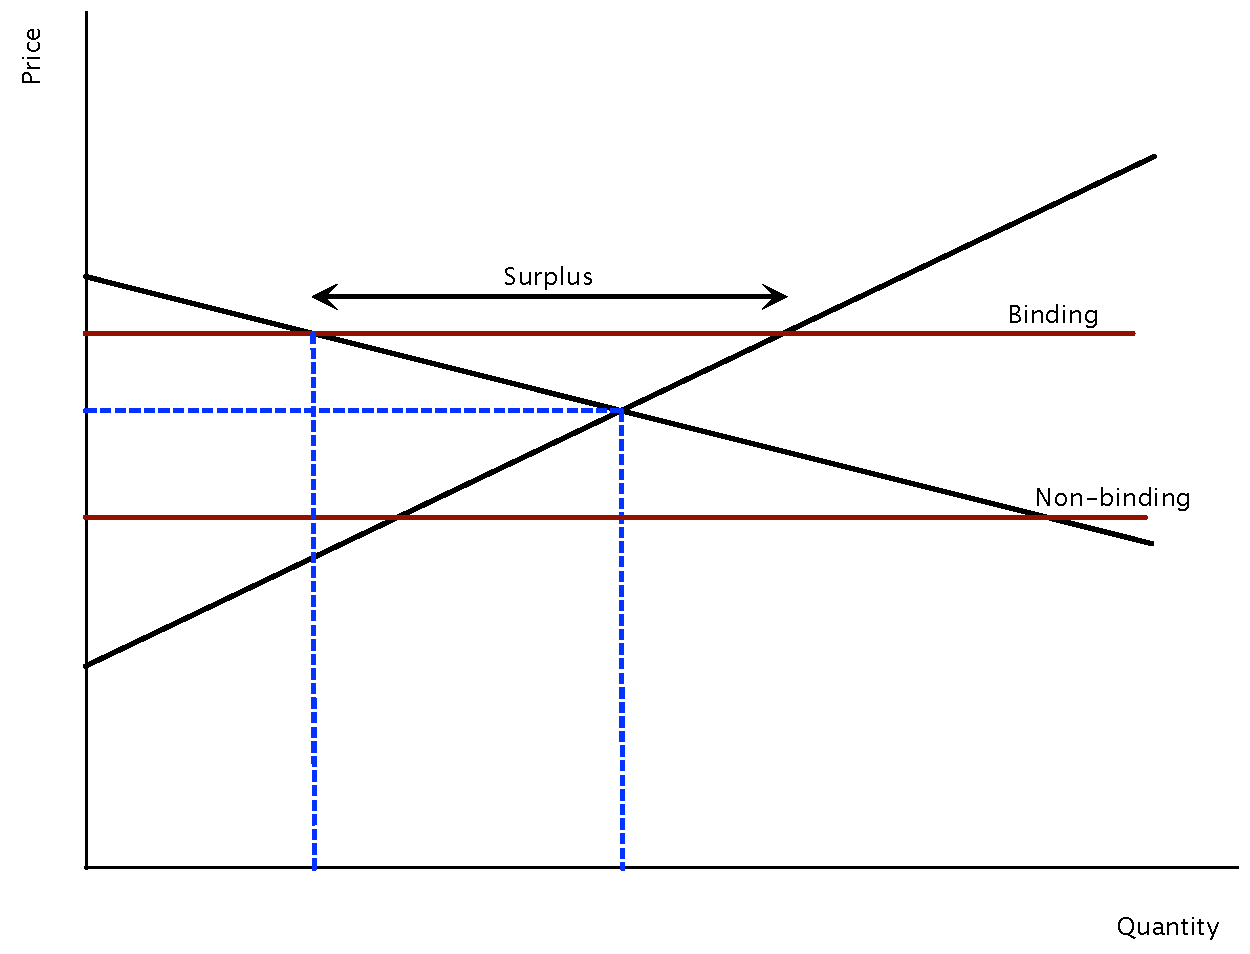
\includegraphics[scale=.40]{plot35.pdf}
			\caption{Price Floors}
		\end{figure}
		
	
	If the government sets a price floor above the market price, then the floor is \dd{binding}.
	\\
	
	If the government sets a price floor below the market price, then the floor is \dd{non-binding}.
	\\
	
	In the case of a binding price floor, once the price in the market hits the floor it cannot decrease any further by law. Therefore, if the price floor is binding, the market price equals the price floor.
	\\
	
	At this price, we have that \dd{$Q_S$} is greater than \dd{$Q_D$}. Thus, there is a \dd{surplus}.
	\\
	
	Due to this, some mechanism for rationing will develop. Two potential ones are
	\begin{enumerate}
		\setlength{\itemsep}{15pt}
		\item \ddp{Sellers who appeal to personal bias of buyers may be better able to sell the good.}
		\item \ddp{Sellers may try to differentiate by increasing quality (wasteful).}
	\end{enumerate}
	\vspace{10pt}
	
	Again, these rationing mechanisms are undesirable.
	\\
	
	\subsubsection*{Welfare Considerations}
	
	
	Consider a market before the introduction of a binding price floor and afterwards:
	
		\begin{figure}[H]
			\centering
			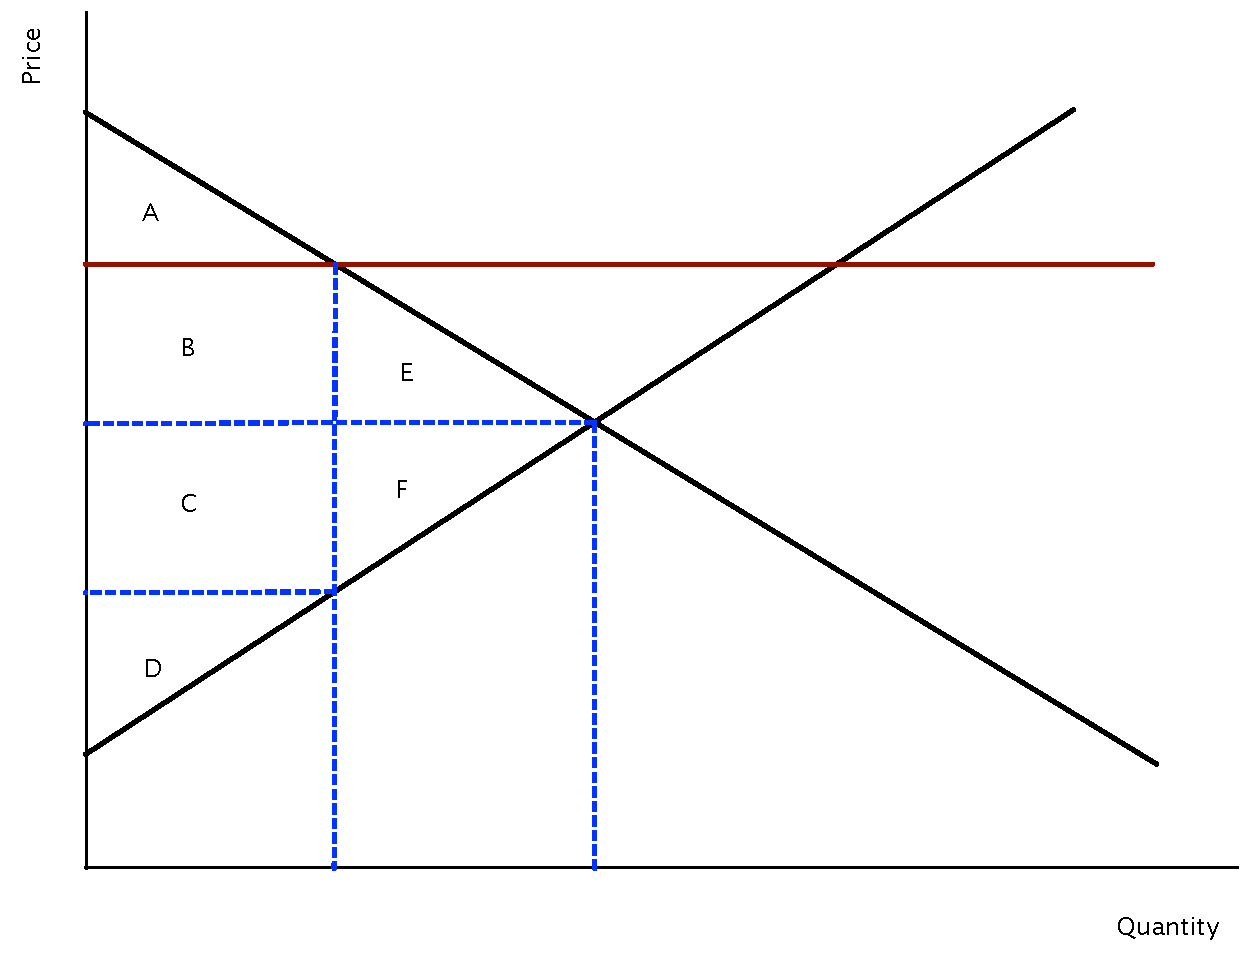
\includegraphics[scale=.40]{plot37.pdf}
			\caption{Price Floors and Welfare}
		\end{figure}
		
	
	After the price floor is introduced, the market price is $P_F$. Buyers and sellers are now paying and receiving \dd{more} than before. Moreover, the number of transactions that are taking place has \dd{decreased}.
	\\
	
	Again, we see that total surplus decreases due to the price control and the deadweight loss is represented by \dd{E + F}.
	\\
	
	\subsubsection*{Application: The Minimum Wage}
	
	
	A labor market consists of workers that determine the supply of labor and firms that determine the demand for labor. The price of labor is the wage that workers receive and firms pay. 
	\\
	
	A labor market with a minimum wage above the equilibrium wage (an example of a binding \dd{price floor}) looks like this:
	
		\begin{figure}[H]
			\centering
			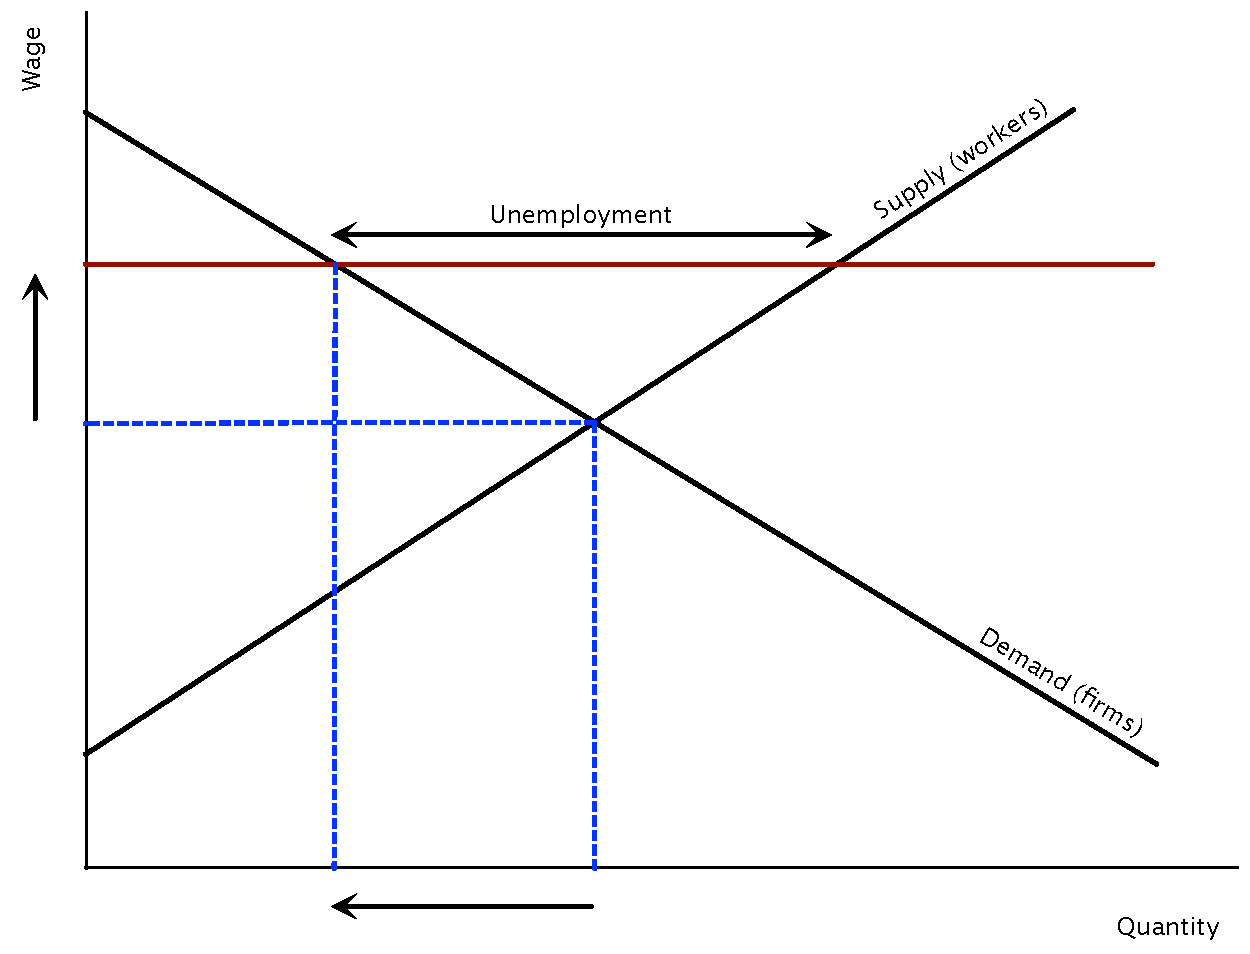
\includegraphics[scale=.40]{plot39.pdf}
			\caption{Market for Labor}
		\end{figure}
		
	
	As usual with a binding price floor, there will be a \dd{surplus}. In the market for labor, this is called \dd{unemployment}.

	
	\begin{exmp} 
		Refer to Figure \ref{fig3}. What are the total wage payments made to workers at the equilibrium wage? Suppose a minimum wage of \$8.00 is enacted. What are the total wage payments made to workers in this case?
	
	\begin{figure}[H]
		\centering
		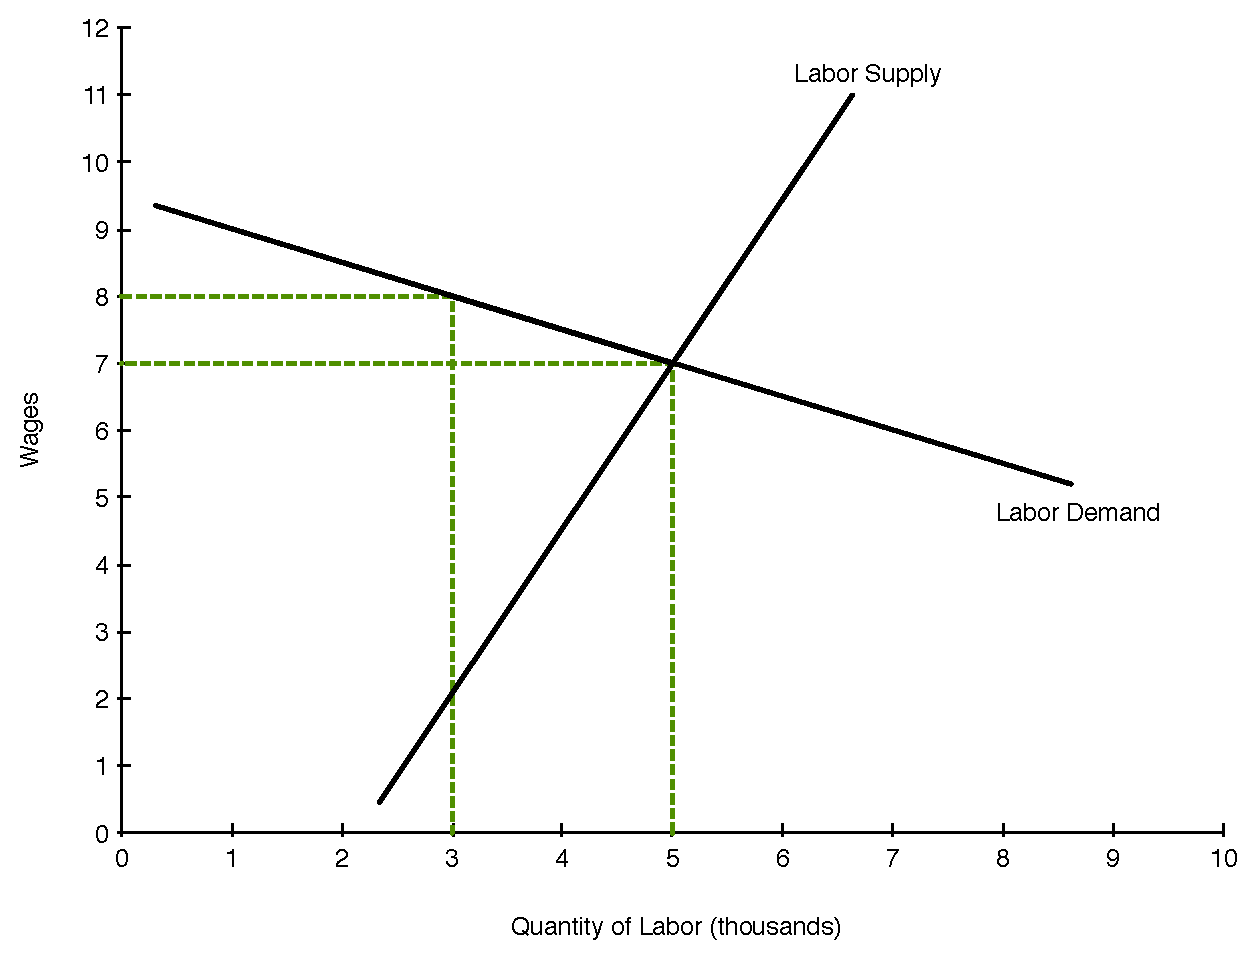
\includegraphics[scale=.4]{notes05_plot1.pdf}
		\caption{Labor Market and Wage Payments}
		\label{fig3}
	\end{figure}
	
\end{exmp}

	\ddp{At eq. wage: $7\times 5,000 = \$35,000$.\\
		At min wage: $8\times 3,000 = \$24,000$.}
	
	\subsection{Taxes}
	
	
	\defn{Tax incidence:} \ddp{The manner in which the burden of a tax is shared among participants in a market. \\}
	
	Taxes can be levied on either (1) sellers or (2) buyers. 
	
		\begin{figure}[H]
			\centering
			\caption{Taxes}
			\begin{subfigure}{.5\textwidth}
				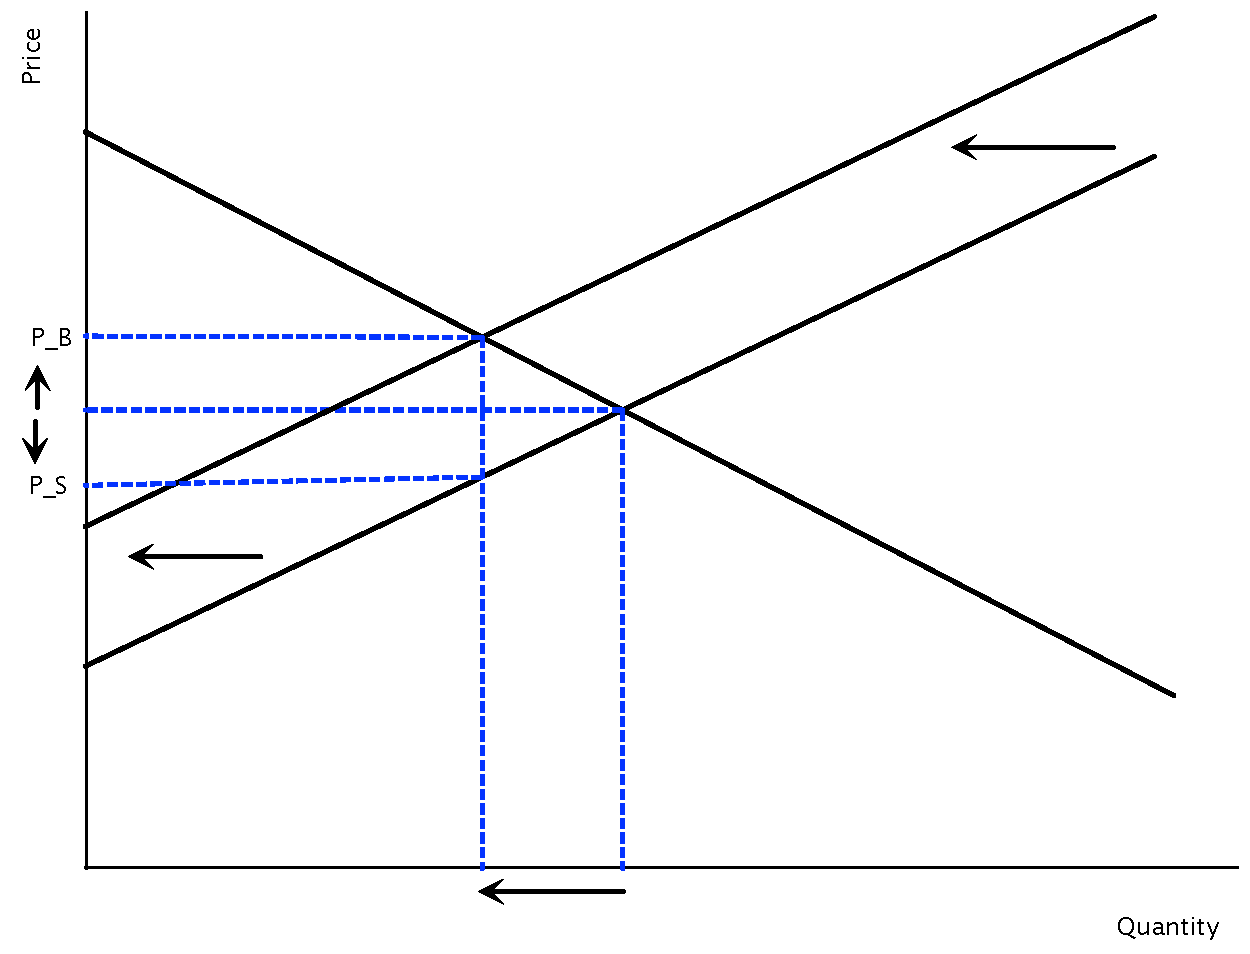
\includegraphics[scale=.25]{plot40.pdf}
				\caption{Tax on Sellers}
			\end{subfigure}%
			\begin{subfigure}{.5\textwidth}
				\centering
				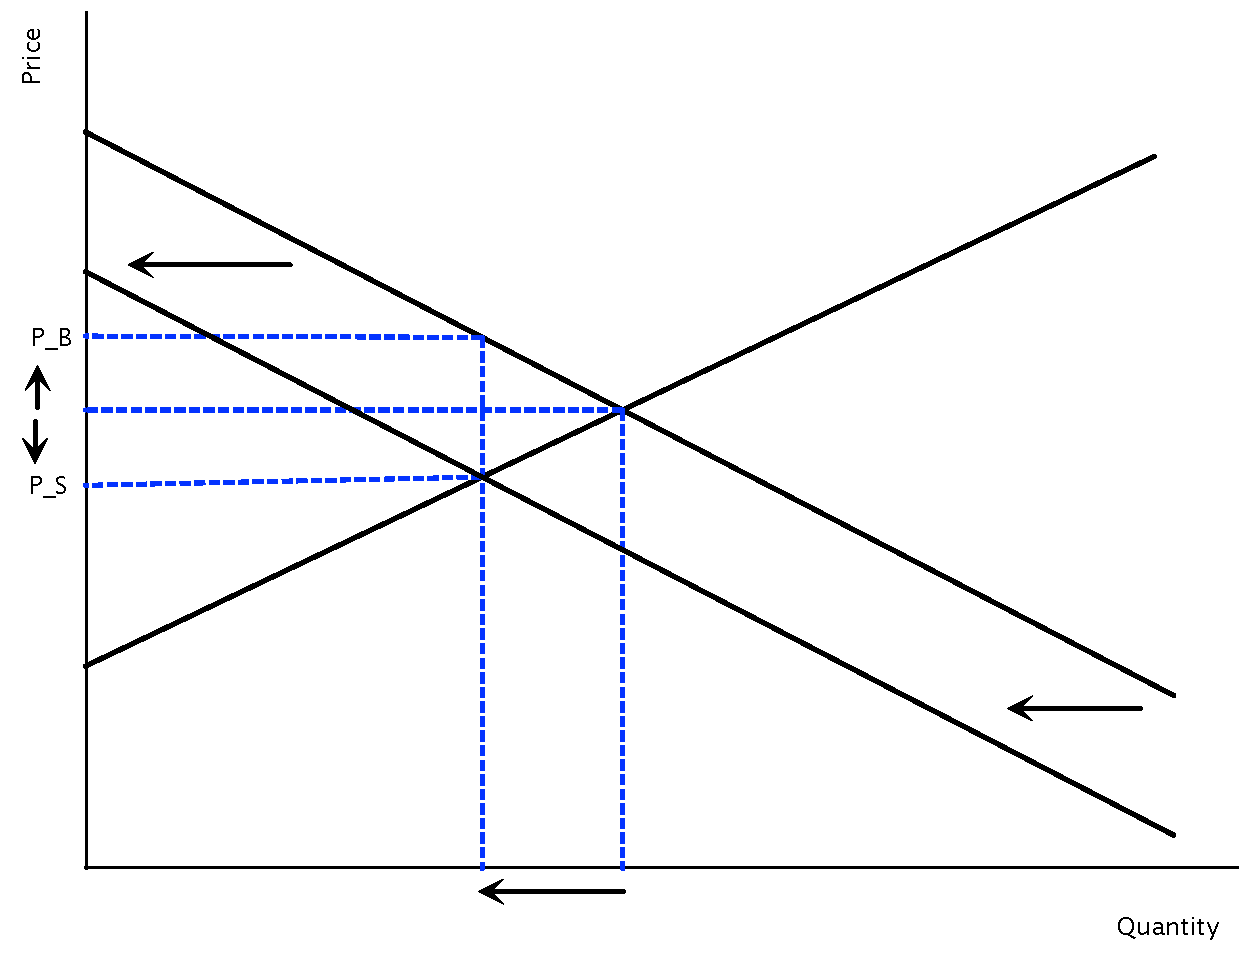
\includegraphics[scale=.25]{plot41.pdf}
				\caption{Tax on Buyers}
			\end{subfigure}
		\end{figure}
	
	Insights:
	\begin{enumerate}
		\setlength{\itemsep}{15pt}
		\item \ddp{Taxes discourage market activity.}
		\item \ddp{Buyers and sellers share the burden of taxes. The price buyers pay increases, and the price sellers receive decreases.}
		\item \ddp{Taxes levied on buyer and sellers are equivalent.}
	\end{enumerate}
	
	\subsubsection*{Elasticity and Tax Incidence}
	
	
	The way the burden of the tax is split depends on the relative elasticities of supply and demand. 
	
	\begin{figure}[H]
		\centering
		\caption{The Tax Burden}
		\begin{subfigure}{.5\textwidth}
			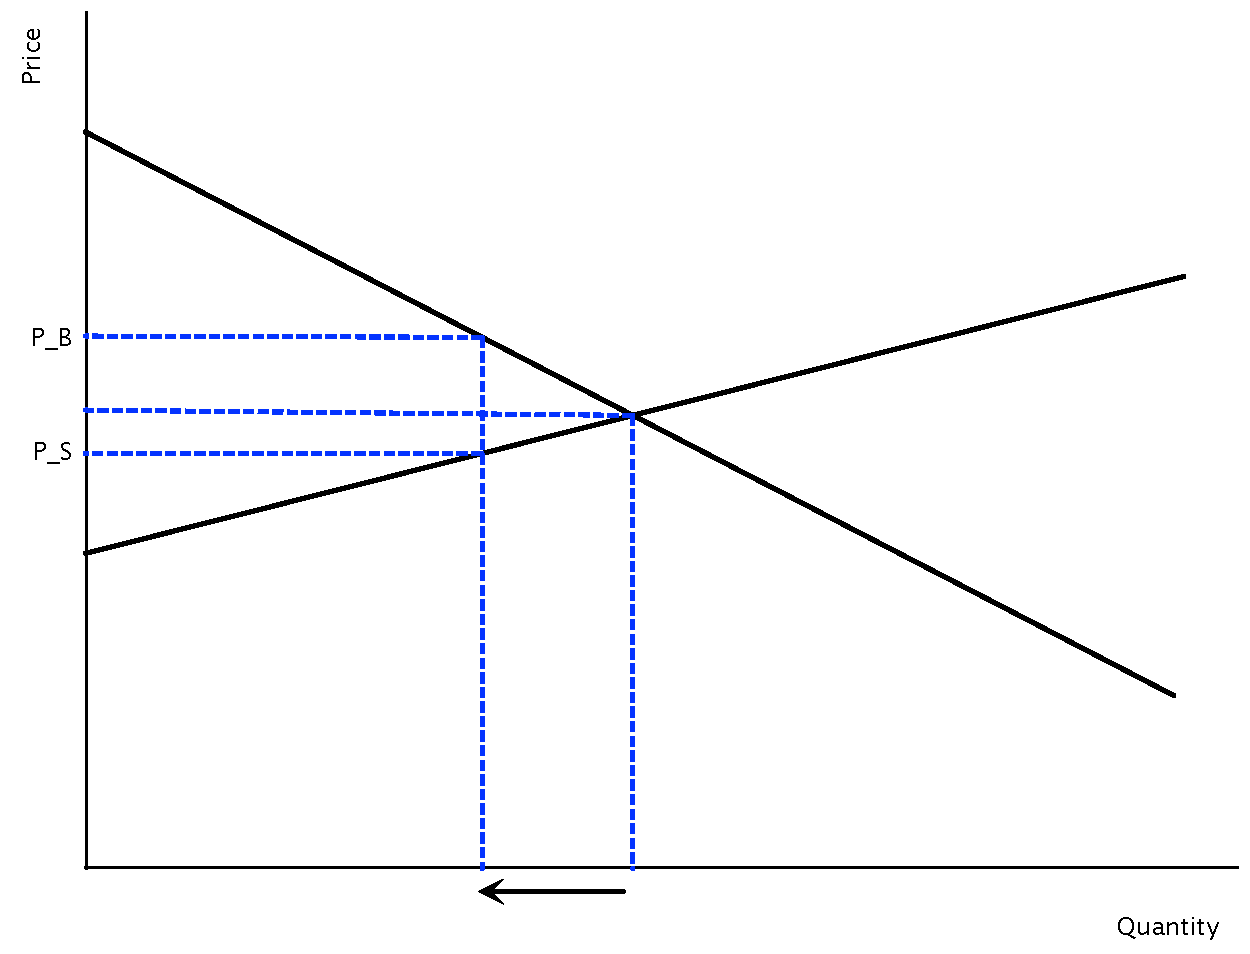
\includegraphics[scale=.25]{plot42.pdf}
			\caption{Elastic Supply}
		\end{subfigure}%
		\begin{subfigure}{.5\textwidth}
			\centering
			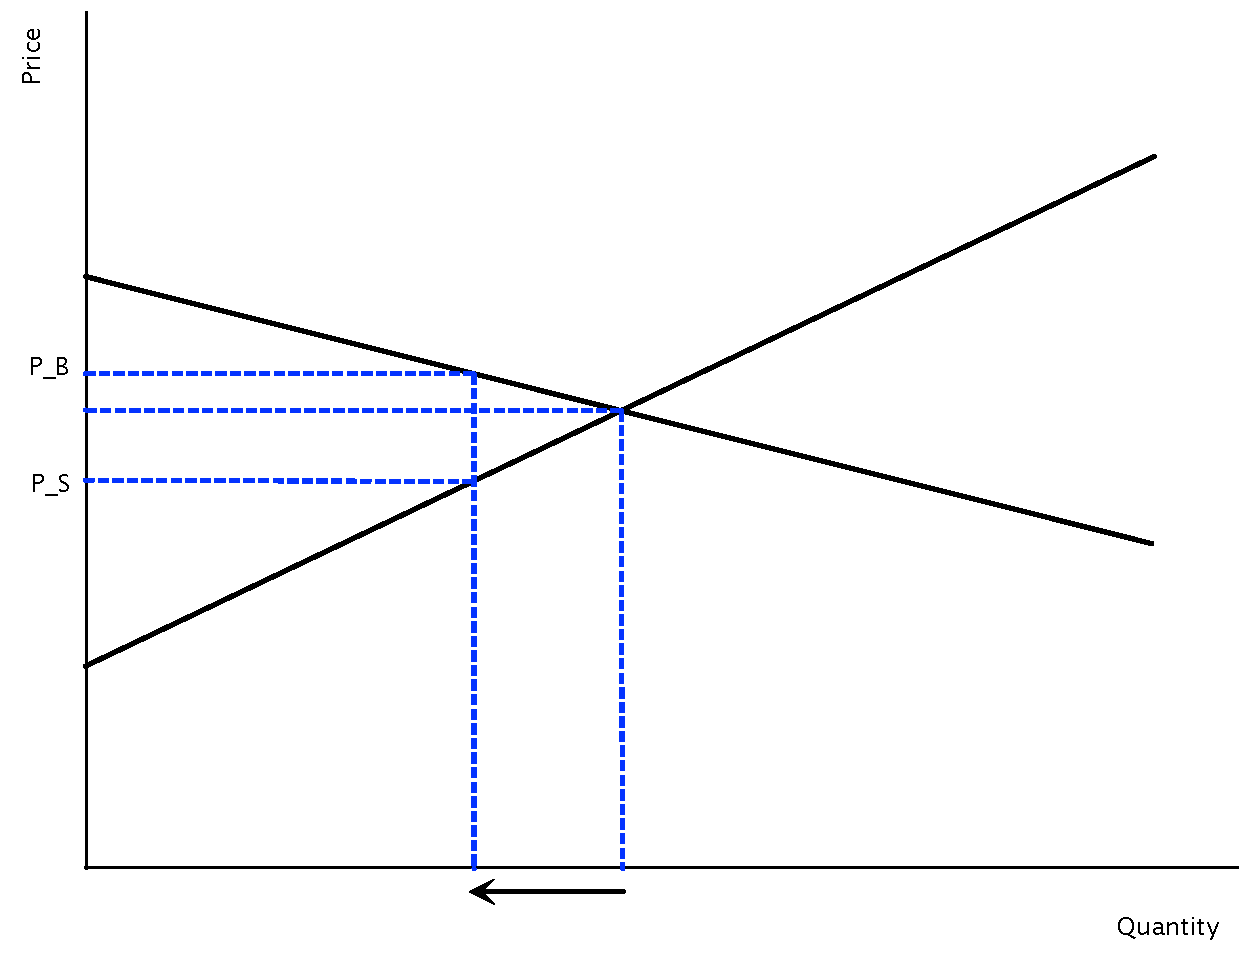
\includegraphics[scale=.25]{plot43.pdf}
			\caption{Elastic Demand}
		\end{subfigure}
	\end{figure}
	
	The tax burden falls more heavily on the side that is \dd{less} elastic.
	
	\ddp{\\ The side with fewer alternatives is less willing to leave the market and so has to bear more of the burden.}
	
	
	\subsubsection*{Welfare Considerations}
	
	When the government levies a tax, it collects \dd{tax revenue}. Though this benefit accrues to those on whom the revenue is spent and not the government itself, we use this to measure the public benefit from the tax. Tax revenue is simply \dd{$\tau \times Q_{\tau}$}. 
	
		\begin{figure}[H]
			\centering
			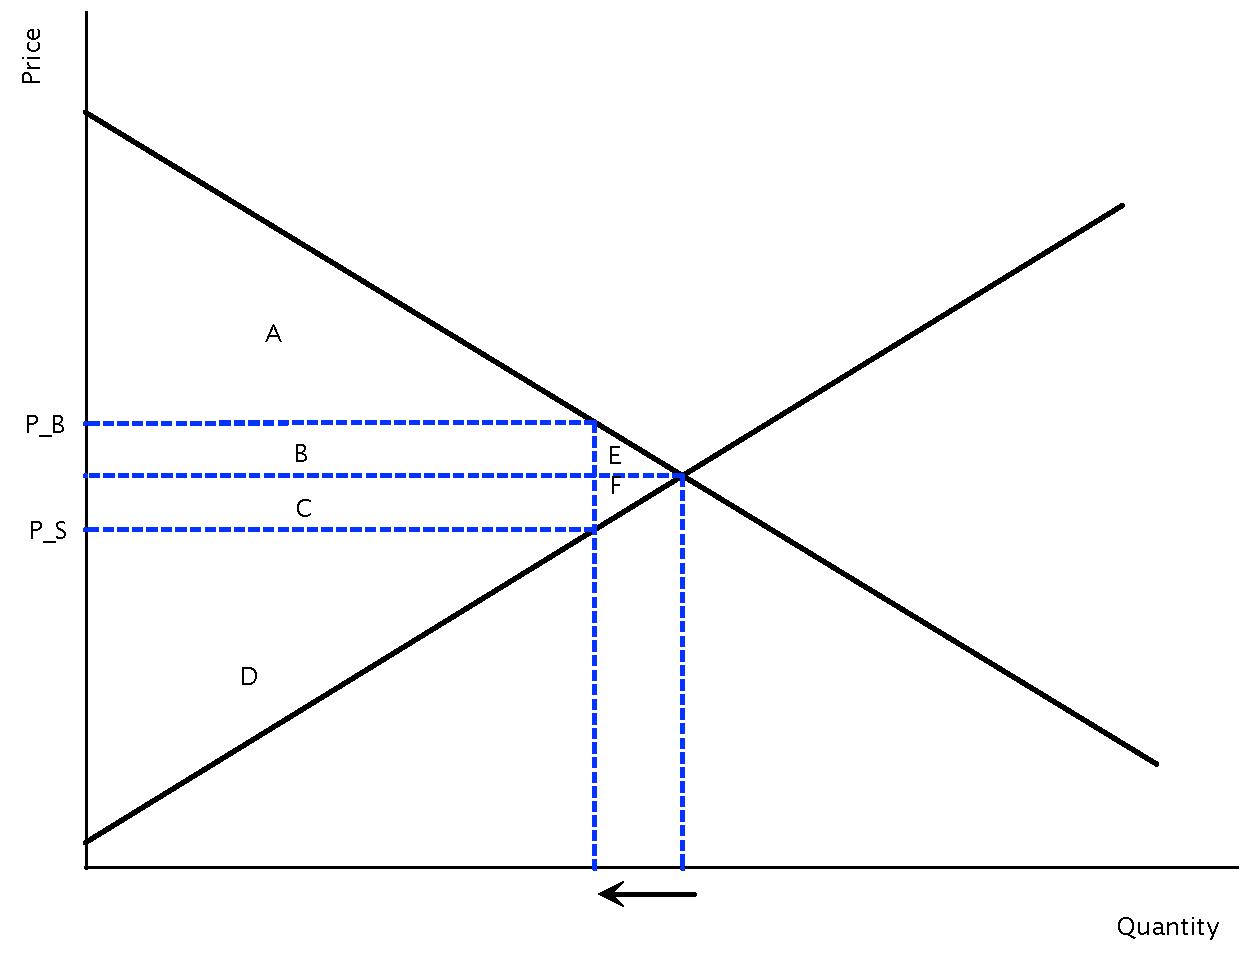
\includegraphics[scale=.3]{plot44.pdf}
			\caption{Taxes and Welfare}
		\end{figure}

	
	By increasing the price buyers pay and decreasing the price sellers receive, a tax \dd{reduces} consumer and producer surplus. Moreover, total surplus \dd{decreases} because the tax revenue earned by the government is \dd{outweighed} by the decreases in CS and PS. Thus, taxes lead to a deadweight loss.
	\\
	
	The decrease in total surplus is due to \dd{unrealized gains from trade}.
	\\
	
	The driving factor behind the size of the deadweight loss is the \dd{elasticity} of supply and demand. The \dd{greater} the elasticities of supply and demand, the \dd{greater} the DWL of a given tax will be.
	
	\ddp{\\ Buyers and sellers are more able to move away from the market, so there are fewer transactions taking place. This leads to more unrealized gains from trade.}
	
		\begin{figure}[H]
			\centering
			\caption{Taxes, Elasticity, and DWL}
			\begin{subfigure}{.5\textwidth}
				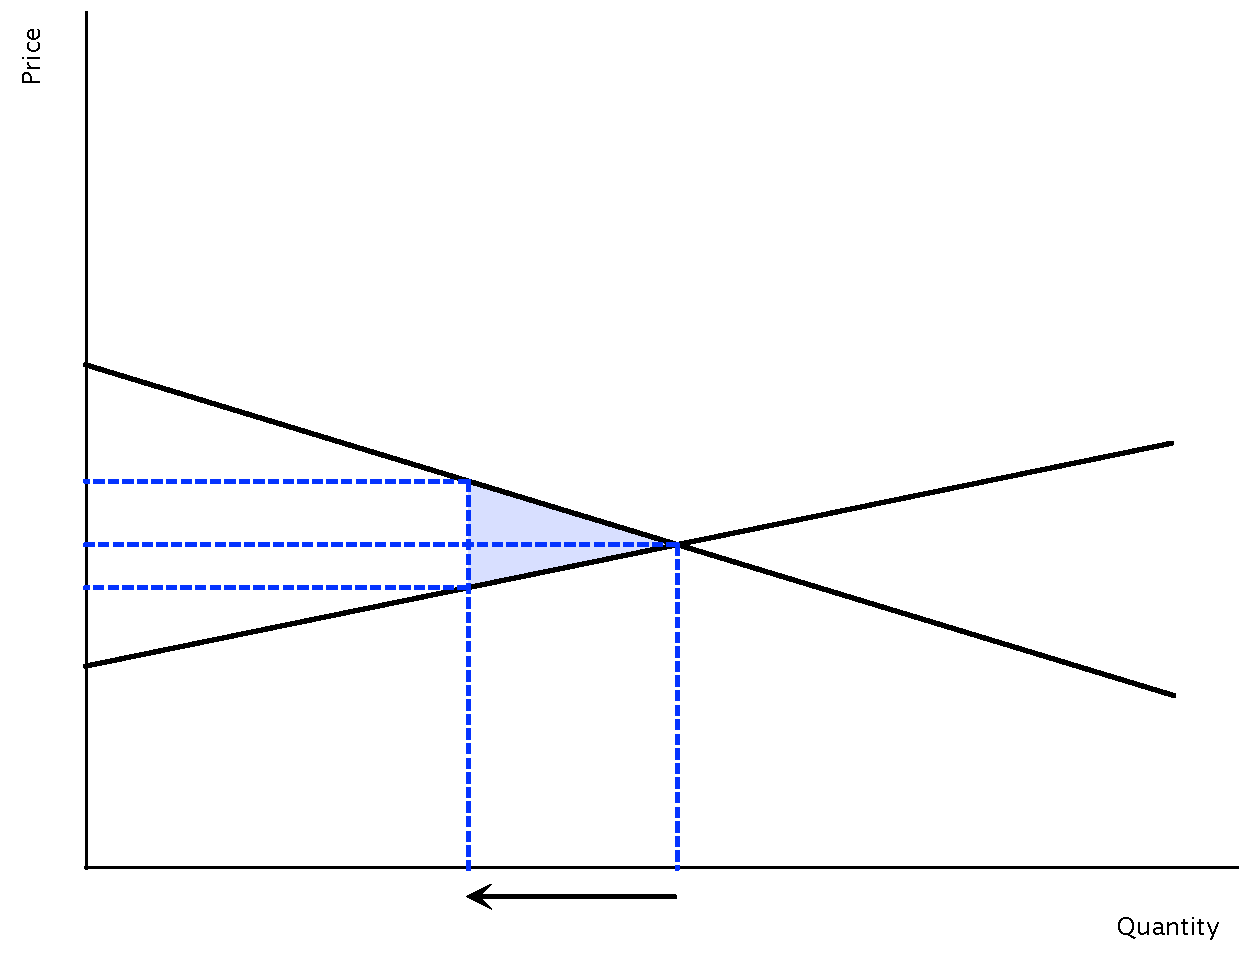
\includegraphics[scale=.25]{plot45.pdf}
				\caption{Elastic Supply and Demand}
			\end{subfigure}%
			\begin{subfigure}{.5\textwidth}
				\centering
				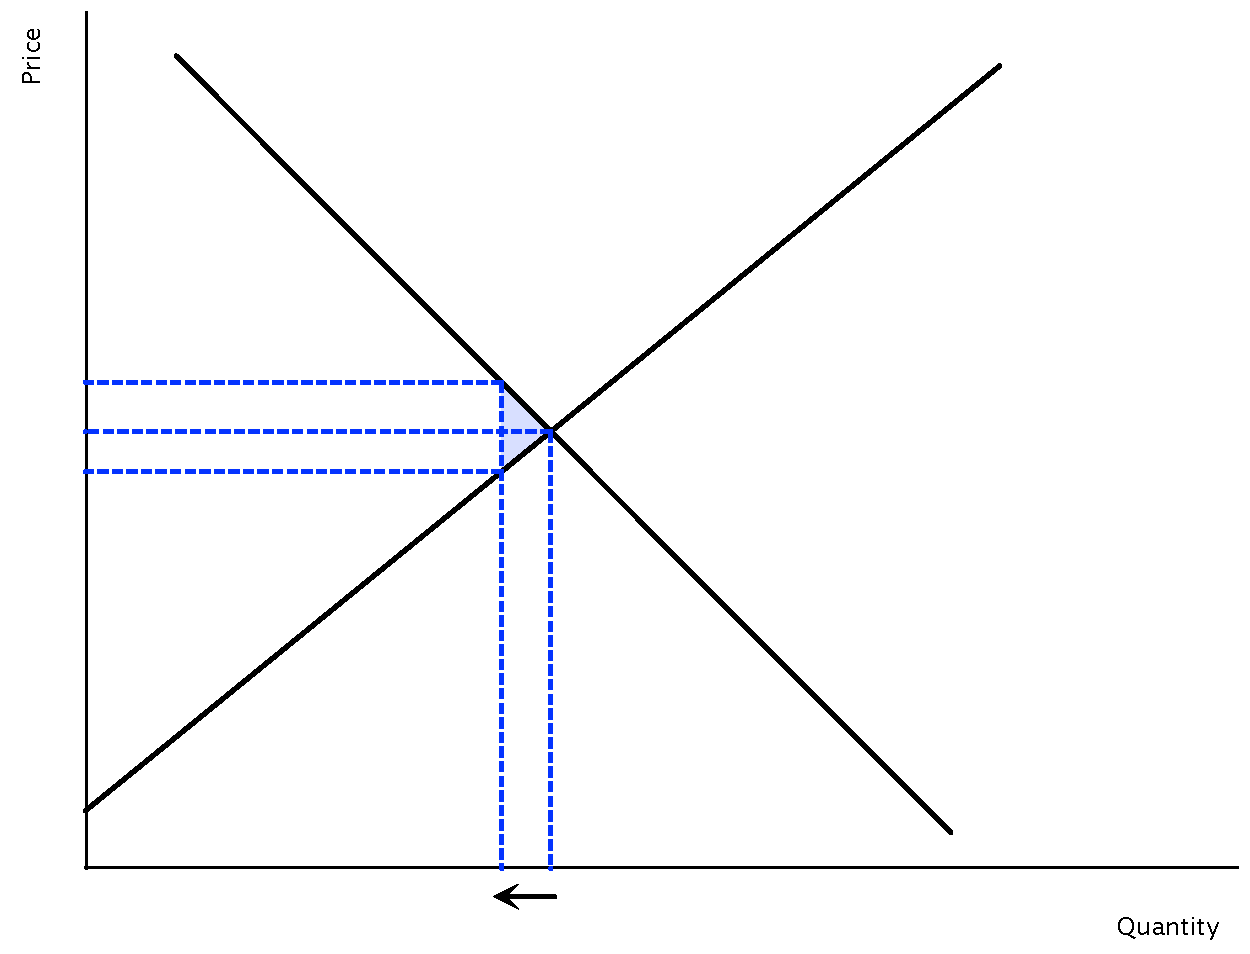
\includegraphics[scale=.25]{plot46.pdf}
				\caption{Inelastic Supply and Demand}
			\end{subfigure}
		\end{figure}
		
	
	For a given supply and demand curve, the DWL of the tax always \dd{increases} as the tax increases, while the amount of tax revenue collected \dd{increases} initially as the tax increases, but eventually \dd{decreases} as the tax continues to increase.
	
		\begin{figure}[H]
			\centering
			\caption{Taxes, DWL, and Tax Revenue}
			\begin{subfigure}{.3\textwidth}
				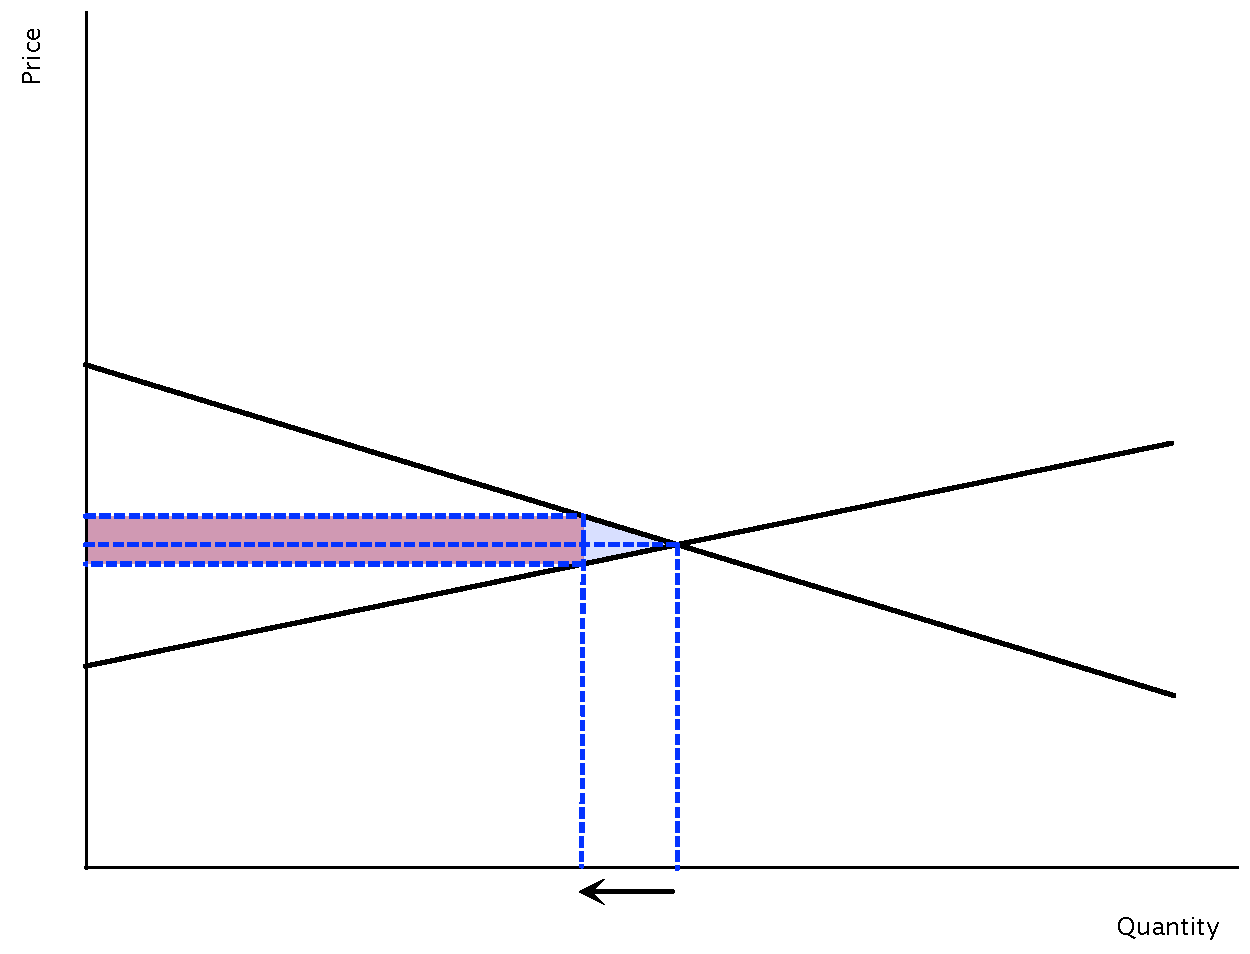
\includegraphics[scale=.2]{plot47.pdf}
				\caption{Small Tax}
			\end{subfigure}%
			\begin{subfigure}{.3\textwidth}
				\centering
				\includegraphics[scale=.2]{plot48.pdf}
				\caption{Medium Tax}
			\end{subfigure}
				\begin{subfigure}{.3\textwidth}
					\centering
					\includegraphics[scale=.2]{plot49.pdf}
					\caption{Large Tax}
				\end{subfigure}
		\end{figure}
		
	
	\newpage
	
	\section{Externalities}
	
	\textbf{Principle 7: Governments Can Sometimes Improve Market Outcomes}
	\\
	
	The purpose of this section is to see why markets sometimes fail to allocate resources efficiently and how government policies can improve such allocations.
	\\
	
	\defn{Externality:} \ddp{The uncompensated impact of one agent's actions on the well-being of a bystander.\\}
	
	
	Externalities can have adverse effects (\dd{negative}) or beneficial impacts (\dd{positive}).
	\\
	
	Because buyers and sellers do not take into account the external effects of their actions, the market equilibrium is \dd{inefficient} when there are externalities.
	
	\ddp{\\ In the presence of an externality, society's interest extends beyond the well-being of market participants.}
	
	\subsection{Negative Externalities}
	
	The idea behind negative externalities is that there is some \dd{external cost} is not taken into account. There is some \dd{private cost} of producing, while the cost to society is referred to as the \dd{social cost}. The cost to society is given by \dd{private cost + external cost}.
	
		\begin{figure}[H]
			\centering
			\includegraphics[scale=.4]{plot50.pdf}
			\caption{Negative Externality}
		\end{figure}
	
	The social-cost curve is \dd{above} the supply curve because it takes into account the external costs imposed on society.
	
	\subsubsection*{Welfare Considerations}
	
	
	Consider a market with a negative externality:
	
	\begin{figure}[H]
	\centering
	\includegraphics[scale=.4]{plot51.pdf}
	\caption{Negative Externalities and Welfare}
	\end{figure}

	
	We see that the optimum amount produced is given by the intersection of the \dd{social cost curve} and the \dd{demand curve}. At quantities below $Q^{**}$, the value to consumers is \dd{greater} than the social cost, while at quantities above $Q^{**}$ and below $Q^*$, the value to consumers is \dd{less} than the social cost.
	\\
	
	Thus, with a negative externality we have that the market equilibrium quantity produced is 
	\\
	\dd{greater} than the socially optimal quantity. 
	\\
	
	\begin{exmp} 
		Refer to Figure \ref{fig4}. What is the per-unit external cost? The total external cost at the market equilibrium? What is total surplus at the market equilibrium? The deadweight loss? What is the efficient quantity in this market?
	
	\begin{figure}[ht!]
		\centering
		\includegraphics[scale=.45]{notes06_plot1.pdf}
		\caption{Market for Floor Cleaner}
		\label{fig4}
	\end{figure}
	\end{exmp}
	
	\ddp{Per-unit EC = \$3. $Q^*$ = 100. TEC = $\$6\times 100 = \$600$. $DWL = (1/2)\cdot6\cdot15 = \$45.$ $Q^{**} = 85$. }
	
	\subsection{Positive Externalities}
	
	On the other hand, some actions yield benefits to third parties. In cases such as this, we have positive externalities.
	\\
	
	In this case, there is some value that people partaking in an activity receive (\dd{private value}).
	\\
	
	Society as whole, however, also gets some \dd{external benefit} from this activity. The sum of these values is referred to as the \dd{social value}. 
	\\
	
	\begin{figure}[H]
			\centering
			\includegraphics[scale=.35]{plot52.pdf}
			\caption{Positive Externality}
	\end{figure}
	
	The demand curve does not reflect the value to society. The social value is \dd{greater} than the private value, and so the social-value curve is above the demand curve.
	
	\subsubsection*{Welfare Considerations}
	
	
	Just like with a negative externality, the equilibrium market quantity is \dd{inefficient} in the presence of a positive externality.
	\\
	
		\begin{figure}[H]
			\centering
			\includegraphics[scale=.35]{plot53.pdf}
			\caption{Positive Externalities and Welfare}
		\end{figure}
	
	The optimum amount produced is given by the intersection of the \dd{social value curve} and the \dd{supply curve}. 
	\\
	
	For all quantities below $Q^{**}$, the social value is \dd{greater} than the private cost.
	\\
	
	Thus, with a positive externality we have that the market equilibrium quantity produced is
	\\
	\dd{less} than the socially optimal quantity. 
	
	\subsection{Correcting Inefficiencies}
	
	If the presence of externalities distorts markets and makes them inefficient, how can the government (or private parties) correct this?
	
	\subsubsection*{Public Policies}
	
	
	Solution 1: \ddp{Command \& control policies (i.e., regulation)}
	\\
	
	Other solutions rely on \dd{market-based} policies. The goal is to align private incentives with social efficiency. \ddp{(``internalizing the externality'')}
	\\
	
	Solution 2: \ddp{Corrective tax or subsidy}
	\\
	
	To align private costs (values) with social costs (values), the per-unit tax (subsidy) must be equal to the \dd{per-unit external cost (benefit)}.
	\\
	
	Solution 3: \ddp{Tradable permits - create markets to trade rights to engage in some activity.}
	\\

	\begin{exmp} 
		
		There are two firms in Candyland, and each one pollutes as shown in Table \ref{pollution}.
	
	\begin{table}[H]
		\caption{Pollution by Firms in Candy Land}
		\label{pollution}
		\centering
		\begin{tabular}{ c|c|c}        
			
			Firm   & Initial Pollution Level  & Cost of Reducing Pollution (per unit)\\
			\hline
			Lolly LLC & 425 units & \$15 \\
			Gloppy Inc. & 300 units & \$10 \\
		\end{tabular}
	\end{table} 
	
	
	\begin{enumerate}
		\item The government wishes to reduce pollution by 400 units and mandates each firm reduce their pollution level by 200 units. How much is each firm polluting now? What is the total cost of reducing pollution in this case?
		\blank{}
		\blank{}
		\ddp{\\ Lolly reduces pollution by 200 units. Cost = \$15 $\times$ 200 = \$3,000. \\
			Gloppy reduces pollution by 200 units. Cost = \$10 $\times$ 200 = \$2,000. \\
			Total pollution = $\underbrace{225}_{\text{Lolly}}$ + $\underbrace{100}_{\text{Gloppy}}$ = 325 units. Total cost = \$5,000.}
		\item Instead, the government gives Lolly 200 pollution permits and Gloppy 125 permits that they can trade with each other. The firms decide to set a price of \$12/permit. How much would each firm pollute? What would be the total cost of reducing pollution?
		\ddp{\\ Lolly will buy all the permits from Gloppy (high-cost polluter buys from low-cost polluter). Lolly will have 325 permits, Gloppy will have 0. \\\\	
			Lolly: Buys 125 permits. Cost of permits = \$12 $\times$ 125 = \$1,500. Able to pollute 325 units, but still has to reduce pollution by 100 units. Cost of reducing pollution = \$15 $\times$  100 =\$1,500. Total cost to Lolly = \$3,000. \\\\
			Gloppy: Sells 125 permits. Revenue = \$12 $\times$ 125 = \$1,500. Has 0 permits, so must reduce pollution by 300 units. Cost of reducing pollution = \$10 $\times$ 300 = \$3,000. Net cost to Gloppy = \$3,000 - \$1,500 = \$1,500. \\\\
			Total pollution = $\underbrace{325}_{\text{Lolly}}$ + $\underbrace{0}_{\text{Gloppy}}$ = 325 units. Total cost = \$4,500.}
	\end{enumerate}
	\blank{}
	\blank{}
	
	Firms with a high cost of reducing pollution will \dd{buy} pollution permits from firms with a low cost of reducing pollution. The price of the pollution permits will be \dd{between the two costs}. Regardless of the actual permit price, the total cost of reducing pollution will be \dd{lower} under tradable permits than under a command and control policy.
	
	\end{exmp}
	
	\subsubsection*{Private Solutions to Externalities}
	
	\begin{enumerate}
		\item Moral codes and sanctions \ddp{(e.g., littering, public nudity)}
		\item Charities \ddp{(e.g., alumni donations)}
		\item Business integration \ddp{(e.g., bar and music venue)}
		\item Contracts \ddp{(e.g., outdoor concert hall and bar)}
	\end{enumerate}
	
	\defn{Coase Theorem:} \ddp{If private parties can bargain without costs over the allocation of resources, they can solve externality problems without government intervention.}
	
	\begin{exmp}
		Suppose that Company A's railroad cars pass through Farmer B's corn fields. The railroad causes an externality to the farmer because the railroad cars emit sparks that cause \$1,500 in damage to the farmer's crops. There is a special soy-based grease that the railroad could purchase that would eliminate the damaging sparks. The grease costs \$1,200. Suppose that the farmer has the right to compensation for any damage that his crops suffer. Assume that there are no transaction costs. Which of the following characterizes the efficient outcome?
		
		\begin{enumerate}[(a)]
			\item The railroad will continue to operate but will pay the farmer \$1,500 in damages.
			\item The railroad will purchase the grease for \$1,200 and pay the farmer nothing because no crop damage will occur.
			\item The farmer will incur \$1,500 in damages to his crops.
			\item The farmer will pay the railroad \$1,200 to purchase the grease so that no crop damage
			will occur.
		\end{enumerate}
	\end{exmp} 
	\ddp{(b) The farmer has the rights, so the railroad has to pay compensation. They would rather pay \$1,200 to buy grease for their cars than pay \$1,500 for compensation.\\}
	
	Note: According to the Coase Theorem, the initial distribution of property rights does not matter - the efficient outcome will be reached in any case. However, it does the determine the distribution of economic well-being. The initial distribution of rights determines who pays who in the final bargain.
	
	\begin{exmp}
		If in the example above, the railroad company had the right to emit sparks, what would the efficient outcome be?
	\end{exmp} 
	\ddp{(d) The farmer has to compensate the railroad in order for them not to emit sparks. He will pay \$1,200 rather than incurring \$1,500 in crop damages.}
	
	\subsubsection*{Failure of Private Solutions}
	
	The Coase Theorem only applies when parties have no trouble reaching and enforcing an agreement. The main barrier to this is \dd{transaction costs}. Additionally, the problem becomes more difficult as the number of parties involved increases.
	
	\newpage
	
	\section{Public Goods and Common Resources}
	
	\defn{Excludability:} \ddp{The property of a good whereby a person can be prevented it from using it. \\}
	
	
	\defn{Rivalry:} \ddp{The property of a good whereby one person's use diminishes other people's use.\\}
	
	
	\textbf{Private goods} are those that are \dd{excludable} and \dd{rival}.
	\\
	
	\textbf{Public goods} are those that are \dd{non-excludable} and \dd{non-rival}.
	\\
	
	\textbf{Common resources} are goods that are \dd{non-excludable} and \dd{rival}.
	\\
	
	\textbf{Club goods} are those that are \dd{excludable} and \dd{non-rival}.
	\\
	
	Note that the boundaries between the categories can be fuzzy.
	
	
	\begin{exmp} 
		Consider I-40. If not many people are using it, traffic flows freely. What type of good is this? As more people start using the interstate (e.g., during rush hour), the congestion slows traffic to a halt. What type of good is I-40 now?
	\end{exmp}
	\ddp{Originally: public good. With congestion: common resource}
	
	\subsection{Public Goods}
	
	\defn{Free rider:} \ddp{A person who receives the benefit of a good but avoids paying for it.\\}
	
	
	\defn{Forced rider:} \ddp{A person who pays for a good but receives less in benefits than the costs incurred.\\}
	
	
	The \dd{free-rider} problem prevents the private market from supplying public goods. Providing a public good confers an \dd{external benefit} on those who enjoy the good, but don't have to pay for it. Thus, without government intervention, public goods tend to be \dd{under provided}.
	\\
	
	The main way the government provides public goods is through the use of \dd{subsidies} and \\ \dd{tax revenues}.
	\\
	
	Notable Public Goods:
	\begin{enumerate}
		\item National defense 
		\item Basic research
		\item Poverty reduction
	\end{enumerate}
	
	\subsection{Common Resources}
	
	\subsubsection*{Tragedy of the Commons}
	
	What is the cause of the tragedy? Differences in \dd{social} and \dd{private} incentives. Because of this misalignment, common resources tend to be \dd{overused}.
	\blank{}
	
	Solutions:
	\begin{enumerate}
		\item Regulation
		\item Market-based policies
		\item Establishing property rights
	\end{enumerate}
	
	Establishing property rights can be done by turning the common resource into a private good. 
	\\
	
	Notable Common Resources:
	\begin{enumerate}
		\item Clean air and water
		\item Fish and other wildlife
	\end{enumerate}
	\vspace{5pt}
	
	The driving factor behind the misallocation of resources in markets where externalities are present is the absence of clearly established \dd{property rights}.
	
	
	\begin{exmp} Four roommates are planning to spend the weekend in their dorm room watching old movies, and they are debating how many to watch. Here is their willingness to pay for each film:
	
	
	\begin{table}[ht]
		\centering
		\begin{tabular}{ c|c|c|c|c }        
			
			& Al & Bob & Carlos & Dylan \\
			\hline
			First film & \$7 & \$5 & \$3 & \$2 \\
			Second film & \$6 & \$4 & \$2 & \$1 \\
			Third film & \$5 & \$3 & \$1 & \$0 \\
			Fourth film & \$4 & \$2 & \$0 & \$0 \\
		\end{tabular}
	\end{table} 
	
	\begin{enumerate}[a.]
		\item Within the dorm room, is the showing of a movie a public good?
		\ddp{\\ Yes; non-excluable and non-rival.}
		\item If the cost to rent a movie is \$8, how many movies should they rent to maximize total surplus? If they split the total cost evenly, what is the surplus realized by each person?
		\ddp{\\ Total WTP for each film: \\
			1: 7 + 5 + 3 + 2 = 17 \\
			2: 6 + 4 + 2 + 1 = 13 \\
			3: 5 + 3 + 1 + 0 = 9 \\
			4: 4 + 2 + 0 + 0 = 6 \\
			They should get a movie as long as P $\le$ total WTP $\Rightarrow$ rent 3 movies. Each pays \$6. \\
			Al: Value - cost = 18 - 6 = 12 \\
			Bob: value - cost = 12 - 6 = 6 \\
			Carlos: value - cost = 6 - 6 = 0 \\
			Dylan: value - cost = 3 - 6 = -3 (forced rider) \\
			Total surplus = \$15.}
	\end{enumerate}
	\end{exmp}
	
\newpage	
	
	\section{The Costs of Production}
	
	\defn{Industrial Organization:} \ddp{The study of how firms' decisions about prices and quantities depend on the market conditions they face.\\}
	
	We assume that the goal of a firm is to maximize \dd{profit}. Firms earn revenue from the sale of their output. Moreover, firms also incurs some costs to produce. The market value of the inputs a firm uses in production are the firm's \dd{total costs}.
	\\
	
	Profit ($\Pi$) is given by \dd{$\Pi = TR - TC$}.

	\subsection{Opportunity Costs}
	
	When we talk about a firm's costs of production, we will include \textit{all} the opportunity costs of making its output. 
	\\
	
	The firm's opportunity costs are divided into two pieces:
	\begin{enumerate}
		\itemsep1em 
		\item Explicit costs: \ddp{Input costs that require an outlay of money by the firm.}
		\item Implicit costs: \ddp{Input costs that do not require an outlay of money.}
	\end{enumerate}
	\vspace{.25cm}
	
	Why do we include implicit costs? \ddp{They affect firm decisions -- opportunity costs should be taken into account.}
	\\

	\defn{Economic profit:} \ddp{$TR$ - (explicit costs + implicit costs). \\}
	
	\defn{Accounting profit:} \ddp{$TR$ - explicit costs.\\}
	
	Since economic profit includes implicit costs, it will generally be \dd{lower} than accounting profit.
	
	\subsection{Production Functions and Marginal Products}
	
	\defn{Production Function:} \ddp{Relationship between quantity of inputs used to make a good and the quantity of output.}
	\\
	
	\begin{figure}[H]
			\centering
			\includegraphics[scale=.30]{plot54.pdf}
			\caption{Simplified Production Function}
		\end{figure}
	
	Rational people (and firms) think \dd{on the margin}. With this in mind, the \defn{marginal product} of an input is the \dd{increase} in \dd{output} from an additional unit of input. Notable marginal products:
	\\
	
	$MP_L$ = \ddp{$\frac{\Delta Q}{\Delta L}$}  
	\\
	
	$MP_K$ = \ddp{$\frac{\Delta Q}{\Delta K}$}  
	\\
	
	\begin{exmp}
		
		Consider Table \ref{bluth} below. What is the marginal product of labor of the second worker? The fifth? Draw a graph and show the $MP_L$ at each unit of labor.
	
	\begin{table}[ht]
		\centering
		\caption{Production of Frozen Bananas}
		\label{bluth}
		\begin{tabular}{ c|c|c}        
			
			Number of workers & Output (per day) & MPL \\
			\hline
			0 & 0 & \ddp{---} \\
			1 & 20 & \ddp{20} \\
			2 & 35 & \ddp{15} \\
			3 & 45 & \ddp{10} \\
			4 & 50 & \ddp{5} \\
			5 & 52 & \ddp{2} \\
			6 & 53 & \ddp{1} \\
		\end{tabular}
	\end{table} 
	\end{exmp}
	
	\begin{figure}[H]
		\centering
		\includegraphics[scale=.40]{plot55.pdf}
		\caption{Marginal Product of Labor}
	\end{figure}
	
	
	Properties of the Production Function:
	\begin{enumerate}
		\item \ddp{Increase in inputs increases production.}
		\item \ddp{Diminishing marginal product: MP declines as the number of inputs increases}
	\end{enumerate}
	
	\subsection{The Different Measures of Cost}
	
	\begin{figure}[H]
		\centering
		\includegraphics[scale=.35]{plot56.pdf}
		\caption{Simplified Total Cost Curve}
	\end{figure}
	
	Because of diminishing marginal product, the cost curve becomes steeper as the quantity of output increases. 
	\\
	
	\ddp{As $Q$ increases, producing an additional unit of output requires a lot of additional units of inputs and so is more costly. \\}
	
	\defn{Fixed Costs:} \ddp{Costs that do not vary with the quantity of output produced.\\}

	
	\defn{Variable Costs:} \ddp{Costs that vary with the quantity of output produced.\\}

	
	If a producer does not produce any output his variable costs are \dd{zero}.
	\\
	
	$TC$ = \dd{$FC + VC$}.
	\\
	
	
	
	\defn{Average Total Cost:} \ddp{Cost of making a typical unit of output. $ATC = TC/Q$.}
	\\
	
	\defn{Average Fixed Cost:} \ddp{$=FC/Q$.}
	\\
	
	\defn{Average Variable Cost:} \ddp{$=VC/Q$.}
	\\
	
	ATC $=$ \dd{$\frac{FC + VC}{Q}$} $=$ \dd{$FC/Q + VC/Q$} $=$ \dd{$AFC + AVC$}
	\\
	
	\defn{Marginal Cost:} \ddp{The increase in total costs that arises from producing an extra unit of output.}
	\\
	
	MC $=$ \ddp{$\frac{\Delta TC}{\Delta Q} = \frac{\Delta VC}{\Delta Q}$.} 
	\\
	
	\begin{figure}[H]
		\centering
		\includegraphics[scale=.35]{plot57.pdf}
		\caption{Simplified Cost Curves}
	\end{figure}
	
	Features:
	\begin{enumerate}
		\item Marginal cost: \ddp{Rising marginal costs. Reflects diminishing MP. TC becomes larger as output increases.}
		\blank{}
		\item Average fixed cost: \ddp{Always decreasing since FC are constant.}
		\blank{}
		\item Average variable cost: \ddp{Rising due to diminishing MP.}
		\blank{}
		\item Average total cost: \ddp{U-shaped due to addition of AFC \& AVC. At low $Q$, high $AFC$, low $AVC$ leads to high $ATC$. As $Q$ increases, $AFC$ decreases fast initially while $AVC$ increases at constant rate so $ATC$ decreases. At high $Q$, $AFC$ decreases slowly and increasing $AVC$ becomes dominant effect so $ATC$ rises.}
		\blank{}
	\end{enumerate}
	
	\defn{Efficient scale:} \ddp{The quantity of output that minimizes $ATC$.}
	
	\subsubsection*{Marginal Cost and ATC}
	
	If we are at a level of production where marginal costs are less than average total costs, then average total costs are \dd{decreasing}.
	\\
	
	If we are at a level of production where marginal costs are greater than average total costs, then average total costs are \dd{increasing.}
	
	\blank{}

	\ddp{\\If the next unit of input adds less to production costs than current average, average cost will decrease. If the next unit of input adds more to production costs than the current average, average cost will increase.\\}
	
	As a result, $ATC$ and $MC$ meet at \dd{the minimum of $ATC$}.
	\\
	
	We made the simplifying assumption that firms exhibit decreasing marginal product for all levels of inputs in order to get the main points associated with production and costs across. However, this is not generally the case. Generally, MP increases initially before decreasing after some level of inputs. The production function and cost curves of such a firm would look as follows:
	
		\begin{figure}[H]
			\centering
			\caption{Standard Curves}
			\begin{subfigure}{.5\textwidth}
				\includegraphics[scale=.3]{plot58.pdf}
				\caption{Standard Production Function}
			\end{subfigure}%
			\begin{subfigure}{.5\textwidth}
				\centering
				\includegraphics[scale=.3]{plot59.pdf}
				\caption{Standard Cost Curves}
			\end{subfigure}
		\end{figure}
	
	Properties:
	\begin{enumerate}
		\item \ddp{$MC$ still increases after some $Q$.}
		\item \ddp{$ATC$ still u-shaped.}
		\item \ddp{$MC$ crosses $ATC$ and $AVC$ at their minimum.}
	\end{enumerate}
	
	\subsection{The Short versus Long Run}
	
	In the short run, a firm cannot get rid of its \dd{fixed costs} because they are \dd{sunk}. However, in the long run, these costs become \dd{variable}.
	
	
		\begin{figure}[H]
			\centering
			\includegraphics[scale=.35]{plot60.pdf}
			\caption{Long-Run ATC}
		\end{figure}
	
	At certain quantities produced, the long run average total cost curve demonstrates
	\begin{itemize}
		\itemsep1em 
		\item \defn{Economies of Scale:} \ddp{Property whereby long-run $ATC$ decreases as $Q$ increases.}
		\item \defn{Constant Returns to Scale:} \ddp{Property whereby long-run $ATC$ remains constant as $Q$ increases.}
		\item \defn{Diseconomies of Scale:}  \ddp{Property whereby long-run $ATC$ decreases as $Q$ increases.}
	\end{itemize}
	
	\begin{exmp}
		Julien's Frozen Banana stand has the following ATC schedule:
	
	\begin{table}[ht]
		\centering
		\caption{ATC of Frozen Bananas}
		\begin{tabular}{ c|c}        
			
			Quantity & Average Total Cost \\
			\hline
			600 & \$3.00 \\
			601 & \$3.01 \\
		\end{tabular}
	\end{table} 
	
	He made 600 bananas today and sold them all. He is about to close up shop when someone calls, desperate to escape the heat and buy a banana. She offers to pay \$5.50 for it. Should Julien accept this offer or not? Why?
	\end{exmp} 
	\ddp{$MB = MR = \$5.50.$ $MC = 9.01$. Nope, don't sell since $MC>MB$.}
	
	\begin{exmp} Julien also owns a juice bar, which has the following cost schedule:
	
	\begin{table}[H]
		\centering
		\caption{Production of Mango Juice}
		\begin{tabular}{ c|c|c|c|c|c}        
			
			Quantity & Variable Cost & Total Cost & AVC & ATC & MC \\
			\hline
			0 & \$0 &\$30 & \ddp{---} & \ddp{---} & \ddp{---} \\
			1 & \$10 & \$40 & \ddp{10} & \ddp{40} & \ddp{10} \\
			2 & \$25 & \$55 & \ddp{12.5} & \ddp{27.5} & \ddp{15}\\
			3 & \$45 & \$75 & \ddp{15} & \ddp{25} & \ddp{20} \\
			4 & \$70 & \$100 & \ddp{17.5} & \ddp{25} & \ddp{25} \\
			5 & \$100 & \$130 &  \ddp{20} & \ddp{26} & \ddp{30} \\
			6 & \$135 & \$165 &  \ddp{22.5} & \ddp{27.5} & \ddp{35}\\
		\end{tabular}
	\end{table} 
	
	Calculate the AVC, ATC, and MC for each quantity.
\end{exmp}
	
\newpage
	
	\section{Perfect Competition}
	
	Perfectly competitive markets are characterized by
	\begin{enumerate}
		\itemsep1em
		\item \ddp{Many buyers and sellers in the market}
		\item \ddp{The good/service being provided by sellers is identical}
		\item \ddp{Firms can freely enter/exit the market}
	\end{enumerate}
	\vspace{2pt}
	
	The goal of this lecture is to analyze how individual firms in these types of markets make optimal decisions.

	
	\subsection{Total Revenue and Related Measures}
	
	Total revenue is given by \dd{$P\times Q$}.
	\\
	
	Individual firms in a competitive market are \dd{price takers}, so for any given quantity they sell, the price they sell for is \dd{the market price (constant)}.
	\\
	
	Two measures related to TR:
	\begin{enumerate}
		\itemsep1em
		\item \textbf{Average Revenue:} \ddp{$AR = TR/Q = P\times Q/Q = P$.}
		\item \textbf{Marginal Revenue:} \ddp{$MR = \frac{\Delta TR}{\Delta Q}$.}
	\end{enumerate}
	
	Note:
	\begin{itemize}
		\item For competitive firms, the \dd{price} is fixed. So, when \dd{quantity} increases by one unit, total revenue increases by \dd{the price}. Thus, \textit{for competitive firms \textbf{only}}, the market price is equal to the \dd{marginal revenue} for each firm.
	\end{itemize}
	
	\subsection{Profit Maximization}
	
	The ``benefit'' to a firm of producing an additional unit of output is their \dd{$MR$} and their cost of producing another unit is their \dd{$MC$}. Thus, they will produce as long as \dd{$MR \ge MC$}. 
	\\
	
	Thinking through this another way, we can express the change in total profit from producing an additional unit of output as \dd{$MR - MC$}. If \dd{$MR > MC$}, then profit is \dd{increasing}. On the other hand, if \dd{$MR < MC$}, then profit is \dd{decreasing}. Given this, it must be that profit is maximized where \dd{$MR = MC$}.
	\\
	
	\begin{exmp}
		Refer to Table \ref{donuts}. Suppose Sarah's Donut Shop is a firm in a competitive market, where the price of a box of donuts is \$11. Fill in the blank columns and find the number of boxes that Sarah should sell to maximize profit. What is this profit if her fixed costs are \$12?
	\pagebreak
	\begin{table}[ht]
		\centering
		\caption{Sarah's Donuts}
		\label{donuts}
		\begin{tabular}{ c|c|c|c|c|c}        
			
			Quantity & Price & Variable Cost  & TR & MR & MC \\
			\hline
			0 & \ddp{11} &  \ddp{0} &  \ddp{0} &  \ddp{---} &  \ddp{---} \\
			1 &  \ddp{11} & \$3 &  \ddp{11} &  \ddp{11} &  \ddp{3} \\
			2 &  \ddp{11} & \$8 &  \ddp{22} &  \ddp{11} &  \ddp{5}\\
			3 &  \ddp{11} & \$15 &  \ddp{33} & \ddp{11}  &  \ddp{7}\\
			4 &  \ddp{11} & \$24 &  \ddp{44} &  \ddp{11}&  \ddp{9} \\
			5 & \ddp{11} & \$35 &  \ddp{55} & \ddp{11} & \ddp{11} \\
			6 & \ddp{11} & \$48 &   \ddp{66}& \ddp{11} & \ddp{13} \\
		\end{tabular}
	\end{table} 
\end{exmp} 
	
	\textbf{Graphical Approach}
	
		\begin{figure}[H]
			\centering
			\includegraphics[scale=.40]{plot61.pdf}
			\caption{Perfectly Competitive Environment}
		\end{figure}
	
	The price line is \dd{horizontal} because the competitive firm is a price taker. 
	\\
	
	Then, the quantity at which profit is maximized is found by tracing down from where the \\ \dd{marginal costs} curve and the \dd{price line (demand curve)} intersect.
	\\
	
	If the quantity is below $Q^*$, then the marginal revenue is \dd{greater than} the marginal cost. Thus, by \dd{increasing} output, the firm can increase its profit. 
	\\
	
	If the quantity were above $Q^*$, then the marginal revenue is \dd{less than} the marginal cost. Thus, by \dd{decreasing} output, the firm can increase its profit. 
	\\
	
	Additionally, we can find profit from a graph. Rewrite profit as 
	\begin{equation*}
	\Pi = \ddp{$TR - TC = PQ - TC = (P-ATC)\times Q$.}
	\phantom{\hspace{9cm}}
	\end{equation*}
	

\begin{figure}[H]
	\centering
	\caption{Firm Profits}
	\begin{subfigure}{.5\textwidth}
		\includegraphics[scale=.3]{plot62.pdf}
		\caption{Firm Making Positive Profit}
	\end{subfigure}%
	\begin{subfigure}{.5\textwidth}
		\centering
		\includegraphics[scale=.3]{plot63.pdf}
		\caption{Firm Making Negative Profit}
	\end{subfigure}
\end{figure}

	
	\subsection{A Firm's Short Run and Long Run Decisions}
	
	\defn{Shutdown decision:} \ddp{A short-run decision to cease production during a specific period of time.\\}
	
	
	\defn{Exit decision:} \ddp{Long-run decision to leave the market.}
	
	\subsubsection*{The Short Run}
	
	In the short run, a firm's \dd{fixed costs} are sunk. Thus, when making its decision to produce in the short run, the firm only considers their \dd{variable costs}. 
	\\
	
	By shutting down, the firm would have a total revenue of \dd{\$0}. But, it would not have to pay its variable costs (though it still has to pay its fixed costs). Given this, the firm will only produce in the short run if \dd{$TR>VC$}. 
	\\
	
	\defn{Shut down rule:} \ddp{Shutdown if $ TR < TC \Rightarrow P < AVC$.}
	
	
			\begin{figure}[H]
				\centering
				\includegraphics[scale=.40]{plot64.pdf}
				\caption{Firm's Short-run Supply Curve}
			\end{figure}
	
	The portion of the $MC$ above the $AVC$ curve characterizes all the quantities at which a firm may produce. This portion of the marginal cost curve is the firm's \dd{short-run supply curve}.
	\\
	
	\begin{exmp} 
		Karlye's Klipz is a hair salon operating in a competitive market. The store's total costs each month are \$7,000. The salon has a yearly lease and pays \$3,000 each month in rent (part of the \$7,000 total monthly costs). All other costs change depending on how many haircuts are provided. The salon's haircuts are provided for \$25 each and they receive 175 patrons a month. What can you say about the salon's short-run decision? What will its profit be?
	\end{exmp}
	\ddp{$FC = 3,000$, $VC = 4000$. $AVC = 4000/175 = \$22.86 < P$, so stay open. $\Pi = \$25 \times 175 - \$7,000 = -\$2,625.$ Profit if firms shuts down = --\$3,000.}
	\blank{}
	
	\subsubsection*{The Long Run}
	
	In the long run, if the firm exits the market then (1) it loses all its revenue, but (2) it saves both its variable costs and fixed costs of production. 
	\\
	
	\defn{Exit rule:} \ddp{Exit if $TR < TC \Rightarrow P < ATC$. \\}
	
	The marginal cost curve above the average total cost curve characterizes the quantities the firm may produce if P > ATC. This portion of the marginal cost curve is the firm's \dd{long-run supply curve}.
	
	\begin{figure}[H]
		\centering
		\includegraphics[scale=.40]{plot65.pdf}
		\caption{Firm's Long-run Supply Curve}
	\end{figure}
	
	From the perspective of a party that wishes to enter the market, they will only do so if the venture will be profitable. Thus, a firm will only enter a market if \dd{$P > ATC$.}.
	\\
	
	\begin{exmp}
		Consider Karlye's Klipz from Example 10.2. What can you say about the salon's long-run decision regarding exiting the market? 
	\end{exmp}
	\blank{}
	\ddp{$ATC = 7,000/175 = \$40 < P$, so exit in long run.}
	
	
	\subsection{Supply in a Competitive Market}
	
	We saw how individual firms in a competitive market make optimal choices. How do these individual firms collectively form the supply curve for a market? 
		
	\subsubsection*{Market Supply in the Short Run}
	
	For any given price, each firm in a competitive market produces the quantity at which P = MC (so long as P > AVC). To derive the market supply curve (in the short run), we add the individual short-run supply curves. 
	\\
	
	Since each firm is identical, the quantity supplied to the market at any given price is the quantity supplied by each firm times the number of firms in the market.
	
	
	\begin{figure}[H]
		\centering
		\caption{Short-run Market Supply}
		\begin{subfigure}{.5\textwidth}
			\includegraphics[scale=.3]{plot66.pdf}
			\caption{Individual Firm}
		\end{subfigure}%
		\begin{subfigure}{.5\textwidth}
			\centering
			\includegraphics[scale=.3]{plot67.pdf}
			\caption{Market Supply}
		\end{subfigure}
	\end{figure}
	
	\subsubsection*{Market Supply in the Long Run}
	
	In the long run, we assume that firms can enter and exit the market. If firms already in the market are profitable, then entrepreneurs outside the market will \dd{enter}. This will \dd{increase} the number of firms in the market, which shifts the supply curve \dd{to the right}. 
	\\
	
	On the other hand, if firms in the market are not profitable, then they will exit the market. This shifts supply \dd{to the left}. 
	\\
	
	Finally, once this process finishes, the firms that do remain in the market make \dd{zero economic profit}, known as \dd{normal profit}.
	\\
	
	From the profit equation, $\Pi = (P - ATC) \times Q$, we see that firms producing output have zero profit if and only if $P = ATC$. Profit is positive if \dd{$P>ATC$} and is negative if \dd{$P<ATC$}.
	\\
	
	If firms in a competitive market set the quantity produced such that $P = MC$, and the process of entry \& exit implies that $P = ATC$, then it has to be that at $Q^*$, $MC = ATC$. 
	\\
	
	We know that if $MC = ATC$, then the firm has to be producing at the \dd{minimum} of ATC. Thus, we have that firms in a competitive market will operate at their \dd{efficient scale} and \dd{$P = \min ATC$} in the long run.
	
	
	\begin{exmp} Suppose that the market for donuts begins at its long run equilibrium. Draw a graph showing the quantity a seller in the market would produce, the MR at this quantity, the average total cost, and the firm's profit. Additionally, draw a graph showing the market for donuts. 
	
	
		\begin{figure}[H]
			\centering
			\caption{Perfectly Competitive Market in Long-run}
			\begin{subfigure}{.5\textwidth}
				\includegraphics[scale=.3]{plot68.pdf}
				\caption{Individual Firm}
			\end{subfigure}%
			\begin{subfigure}{.5\textwidth}
				\centering
				\includegraphics[scale=.3]{plot69.pdf}
				\caption{Market}
			\end{subfigure}
		\end{figure}
		
	
	Now, suppose the surgeon general announces that donuts cause severe health issues. What happens to the market price for donuts? How will firms in the market be affected in the short run? In the long run? Draw graphs to support your answers. 
\end{exmp}

\begin{figure}[ht]
	\begin{subfigure}[b]{0.5\textwidth}
		\centering
		\includegraphics[scale=.30]{plot70.pdf}
		\caption{Market in Short-run}
	\end{subfigure}
	\begin{subfigure}[b]{0.5\textwidth}
		\centering
		\includegraphics[scale=.30]{plot71.pdf}
		\caption{Individual Firms in SR}
	\end{subfigure}
	%        
	
	\begin{subfigure}[b]{0.5\textwidth}
		\centering
		\includegraphics[scale=.30]{plot72.pdf}
		\caption{Market in Long-run}
	\end{subfigure}
	\begin{subfigure}[b]{0.5\textwidth}
		\centering
		\includegraphics[scale=.30]{plot68.pdf}
		\caption{Individual Firms in LR}
	\end{subfigure}
\end{figure}

\newpage	
	
	\section{Monopoly}
	
	Monopolies arise due to lack of competition and thus have a great deal of market power. In contrast to perfectly competitive firms, monopolies are \dd{price makers}.
	
	\subsection{Monopoly Power}
	
	\defn{Monopoly:} \ddp{A fire that is the sole seller of a product without close substitutes.\\}
	
	Fundamental cause: \dd{barriers to entry}.
	\\
	
	Sources of barriers to entry:
	\begin{enumerate}
		\setlength\itemsep{1.5em}
		
		\item Monopoly Resources \ddp{A key resource required for production is owned by a single firm.}
		\item Government-Created Monopolies \ddp{The gov. gives a single firm the exclusive right to produce some good or service.}
		\item \defn{Natural Monopolies}: \ddp{A monopoly that arises because a single firm can supply a good or service to an entire market at a smaller cost than could two or more firms. Important: Experiences economies of scale over the relevant range of output.}
		
			\begin{figure}[H]
				\centering
				\includegraphics[scale=.40]{plot74.pdf}
				\caption{Natural Monopoly Cost Curves}
			\end{figure}
			
	\end{enumerate}
	
	\subsection{Production Decisions}
	
	In contrast to firms in perfect competition, which have a \dd{horizontal demand} due to the goods being perfect substitutes, a monopoly's demand curve is the \dd{market} demand curve. This demand curve is \dd{downward sloping} -- as the price the monopoly charges increases, the quantity demanded of the good decreases.
	\\
	
	The monopoly thus has to balance two effects on total revenue when it increases or decreases the amount it sells:
	
	\begin{enumerate}
		\setlength\itemsep{1em}
		\item The output effect: \ddp{Increasing (decreasing) output tends to increase (decrease) total revenue.}
		\item The price effect: \ddp{Faling (rising) price increases (decreases) total revenue.}
	\end{enumerate}
	\vspace{1em}
	
	\begin{exmp} Suppose a monopolist faces the demand schedule in Table \ref{mono}. Calculate the total revenue the firm can obtain at each price and the MR for each quantity.
	
	\begin{table}[ht]
		\centering
		\caption{Demand Schedule}
		\label{mono}
		\begin{tabular}{ c|c|c|c}        
			
			Price & Quantity & TR & MR  \\
			\hline
			\$21 & 0 &  \ddp{0}&  \ddp{---} \\
			\$20 & 1 & \ddp{21}& \ddp{21}\\
			\$19 & 2 & \ddp{38}& \ddp{17}\\
			\$18 & 3 & \ddp{54}& \ddp{16}\\
			\$17 & 4 & \ddp{68}& \ddp{14}\\
			\$16 & 5 & \ddp{80}& \ddp{12}\\
			\$15 & 6 & \ddp{90}& \ddp{10}\\
			\$14 & 7 & \ddp{98}&  \ddp{8}\\
			\$13 & 8 & \ddp{104}&  \ddp{6}\\
		\end{tabular}
	\end{table}
	\end{exmp} 
	
	
	\subsubsection*{Profit Maximization}
	
		
		\begin{figure}[H]
			\centering
			\includegraphics[scale=.40]{plot75.pdf}
			\caption{Monopolist Environment}
		\end{figure}
	
	Just like firms in perfect competition, the monopolist will choose the level of output where \\ \dd{$MR = MC$}. 
	\\
	
	However, in the case of perfectly competitive firms we had that \dd{$P = MR$}. But in the case of monopolies, it is the case that \dd{$P > MR$}. After choosing the optimal quantity to produce, the price the monopoly will charge is found by tracing up from this optimal quantity up to the \dd{demand curve}.
	\\
	
	Importantly, this implies that the price a monopolist charges is \dd{greater than} the marginal cost at that quantity. This difference is called the \dd{mark-up}, $\mu = $ \dd{$P - MC(Q^*)$}.
	\\
	
	\begin{exmp}
		Suppose the monopolist in Example 11.1 has constant $MC=\$10$/unit and $FC$ = \$20. What is the optimal quantity for the monopolist to produce? What price will the monopolist charge? What is the mark-up? What will its profit be?
	\end{exmp}
	\ddp{If MC=\$10, monopolist will produce 6 units and charge a price of \$15. The mark-up over the marginal cost is \$5. VC of producing 6 units = \$60 since MC is constant \$10. $\Pi = 90 - (60 + 20) = \$10$.}
	\blank{}
	
	\subsection{Welfare Considerations}
	
	A monopolist charges a price above marginal cost. For consumers, this higher price diminishes their surplus. But the firm itself gains surplus by being able to charge this higher price. From a social efficiency stand point, is the quantity that monopolies sell at the one that maximizes total surplus?
	\\
	
	Since the marginal cost curve of the monopolist reflects the costs of production, we see that the socially optimal quantity to produce is where $MC$ equals \dd{demand}.
	
		\begin{figure}[H]
			\centering
			\includegraphics[scale=.40]{plot76.pdf}
			\caption{Monopolists and Welfare}
		\end{figure}
	
	This is efficient because at quantities below $Q^{**}$, the value to buyers is \dd{greater} than the cost to the monopolist. At quantities above $Q^{**}$, the value to buyers is \dd{less} than the cost to the monopolist.
	\\
	
	Therefore, to achieve the efficient outcome the price that should be charged is where the demand curve and the marginal cost curve intersect. That is, just like in the case of perfect competition, the socially efficient quantity is given by where \dd{$P = MC$}. 
	\\
	
	However, a monopolist will produce \dd{less than} the socially efficient quantity due to the mark up over marginal cost.

	
	\subsection{Price Discrimination}
	
	\defn{Price Discrimination:} \ddp{The practice of selling the same good at different prices to different customers.\\}
	
	\begin{enumerate}
		\item A price-discriminating monopolist can charge each consumer a price closer to their willingness to pay. 
		\item This, in turn, allows the monopolist to increase its profits.
		\item In order to price discriminate, the monopolist has to be able to separate consumers by their willingness to pay (e.g., age, geographic region, etc.).
		\item By bringing more consumers into the market, price discrimination potentially increases economic welfare.
	\end{enumerate}
	
	
	In the situation where the monopolist can perfectly price discriminate, then the monopolist will charge each person exactly their willingness to pay and the monopolist gets the entire surplus. 
	\\
	
	If we simplify our graph so that $MC = ATC$ and is constant (i.e., constant per unit costs), we can easily see how this increases total surplus:
	
		\begin{figure}[H]
			\centering
			\includegraphics[scale=.40]{plot77.pdf}
			\caption{Perfect Price Discrimination}
		\end{figure}
	
	When price discrimination is imperfect, as it usually is, the general effect on total welfare is ambiguous. However, it is always true that price discrimination allows a monopolist to increase its profits.
	
	
	
	\subsection{Public Policy}
	
	Because monopolies do not produce the socially efficient quantity, policymakers attempt to respond to this issue in several ways.  
	
	\begin{enumerate}
		\item Increasing competition \ddp{(e.g., antitrust laws)}
		\item Regulation 
		
				\begin{figure}[H]
					\centering
					\caption{Price Regulation}
					\begin{subfigure}{.5\textwidth}
						\includegraphics[scale=.3]{plot78.pdf}
						\caption{Marginal Cost Pricing}
					\end{subfigure}%
					\begin{subfigure}{.5\textwidth}
						\centering
						\includegraphics[scale=.3]{plot79.pdf}
						\caption{Average Total Cost Pricing}
					\end{subfigure}
				\end{figure}
		
		\item Public ownership \ddp{(i.e., government runs monopoly itself)}
		\item Doing nothing
	\end{enumerate}
	
\newpage	
	
	\section{Monopolistic Competition and Oligopoly}
	
	This section looks at firms within industries that have some monopolistic tendencies, but are competitive in some senses as well.
	
	\subsection{Monopolistic Competition}
	
	\defn{Monopolistic Competition:} \ddp{A market structure in which many firms sell products that are similar but not identical.\\}
	
	Monopolistic competition arises in markets with the following attributes:
	\begin{enumerate}
		\setlength\itemsep{1em}
		\item Many sellers \ddp{Many firms competing for the same group of customers.}
		\item Product differentiation \ddp{Product produced is at least slightly different than other firms $\Rightarrow$ Downward sloping demand.}
		\item Free entry and exit \ddp{$\Rightarrow \Pi = 0$.}
	\end{enumerate}
	
	\subsubsection*{The Short Run}
	
	In the short-run, a firm in a monopolistically competitive market chooses its optimal quantity and price just like a monopolist: Find the quantity where \dd{$MR$} and \dd{$MC$} intersect and trace up to the \dd{demand} curve to find the price. 
	\\
	
	The only difference here is the slope of the demand curve: Because consumers in a monopolistically competitive market have numerous substitutes for the product each firm sells, the demand curve is more \dd{elastic}. 
	\\
	
		\begin{figure}[H]
			\centering
			\includegraphics[scale=.40]{plot80.pdf}
			\caption{Monopolistic Competition in Short-run}
		\end{figure}
	
	\subsubsection*{The Long Run}
	
	Due to entry and exit, firms in markets characterized by monopolistic competition make \\ \dd{zero (normal) profit} in the long run. 
	
	\begin{itemize}
		
		
		\item If firms in the industry are making profit, then other firms will enter the market. In this case, the demand faced by \textit{each} firm will \dd{decrease} since the number of products to choose from has increased. Moreover, each demand curve becomes \dd{more} elastic.
		
		\item If firms in the industry are making a loss, then firms will exit the market. In this case, the demand faced by \textit{each} firm remaining will \dd{increase} since the number of products to choose from has decreased. Moreover, each demand curve becomes \dd{less} elastic.
		
	\end{itemize}
	
	\begin{figure}[H]
		\centering
		\includegraphics[scale=.40]{plot81.pdf}
		\caption{Monopolistic Competition in Long-run}
	\end{figure}
	
	The long run condition is that at the profit maximizing quantity, the demand curve and the average total cost curve are \dd{tangent}.
	\\
	
	Just like in a market with a monopoly, firms in monopolistically competitive markets charge a price that is \dd{greater} than the marginal cost. 
	\\
	
	Just like perfectly competitive markets, the process of entry and exit means that for firms in a monopolistically competitive market the long run the price is \dd{equal} to the average total cost. 
	\\
	
	However, unlike firms in perfect competition, firms in a monopolistically competitive market do not produce at the \dd{social optimum} in the long run. The difference between the efficient scale and the quantity produced is called \dd{excess capacity}.
	
	\subsubsection*{Welfare Considerations}  
	
	Because of the markup over marginal costs, some consumers who value the good more than the marginal cost but less than the price will be deterred from purchasing it. As such, the welfare analysis is equivalent to that of a monopolistic firm.
	
		\begin{figure}[H]
			\centering
			\includegraphics[scale=.40]{plot82.pdf}
			\caption{Monopolistic Competition and Welfare}
		\end{figure}
	
	Externalities associated with entry:
	\begin{enumerate}
		\item Product-variety externality \ddp{New firms in the market leads to more differentiated products $\Rightarrow$ Increased surplus to consumers (positive externality)}
		\item Business stealing externality \ddp{New firms steal existing customers and profits from existing firms (negative externality)}
	\end{enumerate}
	\ddp{Thus, we might have too many or too few products.}
	
	
	\subsection{Oligopoly}
	
	\defn{Oligopoly:} \ddp{A market structure in which only a few sellers offer similar or identical products.\\}
	
	Due to the interdependence of the firms in an oligopoly, we will turn to concepts from elementary \textbf{game theory} \ddp{(the study of how people behave in strategic interactions)} in order to analyze how these firms behave. 
	
	
	
	
	\subsubsection*{Duopoly}

	
	\begin{exmp} Table \ref{diamonds} shows the $ATC$ and demand for diamonds. A large share of the world's supply of diamonds comes from Russia and South Africa. Suppose the two countries decide to work together in order maximize total profits. What would be the price and quantity? If they split production evenly, how much would Russia produce and what would be its profits?
		
		\ddp{\\ Under collusion, countries act as a monopolist and produce as long as $MR\ge MC$. $Q^* = 6,000$ at $P^* = 7,000$. $\Pi = (7,000 - 1,000) \times 3,000 = \$18$M for each nation.\\}
			\blank{}
			\blank{}
			\blank{}
			\blank{}
			\blank{}
			
	What would happen to each nation's profit if Russia decided to increase their production by 1,000 and South Africa stuck to the original agreement? What would happen if they both increased their production by 1,000?
		
		\ddp{\\ If Russia deviates, ($P^*,Q^*) = (\$6,000, 7,000)$. $\Pi_R = (\$6,000 - 1,000) \times 4,000 = \$20$M. \\
			SA's profit is $\Pi_{SA} = (\$6,000 - 1,000) \times 3,000 = \$15$M. \\ If they both deviate,  ($P^*,Q^*) = (\$5,000, 8,000)$. $\Pi = (\$5,000 - 1,000) \times 4,000 = \$16,000$ for each.}
	\end{exmp}
	
	\blank{}
	\blank{}
	\blank{}
	\blank{}
	\blank{}
	
	\begin{table}[H]
		\centering
		\caption{Demand Schedule}
		\label{diamonds}
		\begin{tabular}{  c| c | c | c| c| c| c}        
			
			Price & Quantity & ATC & TC & MC & TR &  MR  \\
			\hline
			\$8,000 & 5,000 & \$1,000 & \ddp{5,000,000} & \ddp{---} & \ddp{40,000,000} & \ddp{---}\\
			\$7,000 & 6,000 & \$1,000  & \ddp{6,000,000} & \ddp{1,000} & \ddp{42,000,000} & \ddp{2,000}\\
			\$6,000 & 7,000 & \$1,000  & \ddp{7,000,000} & \ddp{1,000} & \ddp{42,000,000} & \ddp{0}\\
			\$5,000 & 8,000 & \$1,000  & \ddp{8,000,000} & \ddp{1,000} & \ddp{40,000,000} & \ddp{--2,000}\\
			\$4,000 & 9,000 & \$1,000 & \ddp{9,000,000} & \ddp{1,000} & \ddp{36,000,000} & \ddp{--4,000}\\
			\$3,000 & 10,000 & \$1,000 & \ddp{10,000,000} & \ddp{1,000} & \ddp{30,000,000} & \ddp{--6,000}\\
			\$2,000 & 11,000 & \$1,000 & \ddp{11,000,000} & \ddp{1,000} & \ddp{22,000,000} & \ddp{--8,000}\\
			\$1,000 & 12,000 & \$1,000  & \ddp{12,000,000} & \ddp{1,000} & \ddp{12,000,000} & \ddp{--10,000}\\
			
		\end{tabular}
	\end{table} 
	
	
	
	\defn{Collusion:} \ddp{An agreement among firms in a market about quantities to produce or prices to charge.\\}
	
	
	\defn{Cartel:} \ddp{A group of firms acting in unison.\\}
	
	As we saw in our example, the self-interest of each party drives each firm to produce more. Thus, the non-cooperative duopolist output is above the monopolist output level. However, it will still be below that of a perfectly competitive firm's allocation. At some point of production, each firm will have no incentive to either increase or decrease their output level because they are already maximizing profit. 
	\\
	
	\defn{Nash Equilibrium:} \ddp{A situation where agents interacting with each other choose their best strategy given the strategies all other agents have chosen and can do no better by deviating.\\}
	
	In summary, we have that when firms in an oligopoly individually choose their production levels to maximize profit, they produce a quantity \dd{greater} than that produced by a monopoly and \dd{less} than that produced under perfect competition. Additionally, the oligopoly price is \dd{lower} than that of a monopoly and \dd{greater} than the competitive price.
	
	\subsubsection*{The Economics of Cooperation}
	
	
	\begin{exmp}
		Consider the utility gained by Jack and Jill as a result of their decisions to either snitch or keep mum. This is detailed in the table below.
	
	\renewcommand{\gamestretch}{1.5}
	\sgcolsep=25pt
	\begin{figure}[htb]\hspace*{\fill}%
		\begin{game}{2}{2}[Jack][Jill] 
			&  Snitch & Keep Mum \\
			Snitch & $10, 10$ & $30, 0$ \\
			Keep Mum & $0, 30$ & $20, 20$
		\end{game} 
		\hspace*{\fill}%
	\end{figure}
	
	Jack is the \dd{row} player and Jill the \dd{column} player.
	\\
	
	Jack's ``payoff'' is the first number in each box, while Jill's is the second. For example, if Jack decides to snitch and Jill keeps mum, Jack's payoff is \dd{30} and Jill's payoff is \dd{0}.
	\\
	
	Let's look at this game from Jack's perspective: If Jill snitches, he is better off \dd{snitching} as well since \dd{$10 > 0$}. We call this his \dd{best response}. If Jill keeps mum, then Jack is still better off snitching since $30>20$. No matter what Jill does, Jack is better off snitching. This type of strategy is referred to as a \dd{dominant strategy}. 
	\\
	
	\defn{Dominant Strategy:} \ddp{A strategy that is best for a player in a game regardless of the strategies chosen by other players.\\}

	
	A similar analysis for Jill shows that her dominant strategy is to snitch as well. Thus, both parties end up snitching and receive payoffs of 10 and 10, respectively. This outcome is a \dd{Nash equilibrium}.   

	
	\end{exmp} 
	
	\begin{exmp}
		
	Write out the game form of example 12.1, where Russia is the row player and South Africa is the column player. Does either country have a dominant strategy? If there is one, what is the Nash equilibrium of this game?
	
		\renewcommand{\gamestretch}{1.5}
		\sgcolsep=25pt
		\begin{figure}[htb]\hspace*{\fill}%
			\begin{game}{2}{2}[Russia][South Africa] 
				&  \ddp{Produce 3,000} & \ddp{Produce 4,000} \\
				\ddp{Produce 3,000} & \ddp{18,18} & \ddp{15,20}\\
				\ddp{Produce 4,000} & \ddp{20,15} & \ddp{16,16}
			\end{game} 
			\hspace*{\fill}%
		\end{figure}
		
		\ddp{Nash eq. is where each produces 4,000 as each nation's dominant strategy is to produce this amount.}
		
	\end{exmp}
		
	\begin{exmp}
		
		Consider the game below, detailing the payoffs to Dynaco and Synergy when they decide on the size of their research budget. Does either party have a dominant strategy? If so, what is it? What will be the outcome if this game is played once?
	
	\renewcommand{\gamestretch}{1.5}
	\sgcolsep=25pt
	\begin{figure}[htb]\hspace*{\fill}%
		\begin{game}{2}{2}[Dynaco][Synergy] 
			&  Large Budget & Small Budget \\
			Large Budget & \$30M, \$20M & \$70M, \$0 \\
			Small Budget & \$0, \$30M & \$50M, \$40M \\
		\end{game} 
		\hspace*{\fill}%
	\end{figure}
	\end{exmp}
	\blank{}
	\blank{}
	\ddp{Dynaco's dominant strategy is to have a large budget. Synergy has no dominant strategy, but since they know Dynaco will play large budget, their best response is to play large budget. The Nash eq. is (large budget, large budget).\\}
	
	
	Do parties always defect? No. Cooperation between parties is made easier when games are repeated.
	\\
	
	This is usually achieved by specifying what each party will do in order to maximize the payoff to both parties. If either one defects in one period, then the other party imposes some sort of penalty by switching strategies the next period (and potentially forever after). As long as each player cares enough about future payoffs, then they will forgo a one-time gain from defection.
	
\newpage	

\section{Introduction to Macroeconomics}

This section will look at how we measure the total income of a nation -- its gross domestic product. 
\\

GDP measures both the total \dd{income} of everyone in the economy and the total \\ \dd{expenditure} on the economy's output of goods and services. That is, for the economy as whole, \dd{income} must equal \dd{expenditures}. 
\\

\defn{GDP:} \ddp{The market value of all \underline{final} goods and services produced \underline{within} a country during a specific period of time (typically a year).\\}


A closer look:
\begin{itemize}
	\item GDP adds together many different kinds of products into a single measure of economic activity. To do so, it uses \dd{prices}, which reflect the value of goods.
	\item Includes all items produced in the economy and sold \textit{legally} in markets.
	\begin{enumerate}[i.]
		\item Includes market value of housing services. This includes the rental value of owner-owned housing. \ddp{How much a house could be rented for?}
		\item Excludes items produced and sold illicitly and most items that are produced and consumed within a household. \ddp{e.g., prostitution, gambling, tomatoes grown at home}
	\end{enumerate}
	\item GDP \textbf{only} includes the value of final goods. The value of intermediate goods used to produce final goods is not included. An exception to this rule is when an intermediate good is added to a firm's inventory for use or sale at a later date. Thus, additions to inventory \dd{increase} GDP and when the goods are later used or sold, the reductions in inventory \dd{detract} from GDP.
	\item Includes goods and services that are \dd{currently} produced. The sale of a used good is \textbf{not} included. 
	\item Items are included in a nation's GDP only if they are produced \dd{domestically}. The nationality of the producer does not matter.
	\item GDP is usually reported at intervals of a year or a quarter of a year.
\end{itemize}

\begin{exmp} 
	For each of the following, find out how much each transaction contributes to GDP.
	\begin{enumerate}
	\setlength{\itemsep}{1em}
\item	A metal company sells steel to a bicycle company for \$150. The bicycle company uses this steel to produce a bike, which it sells for \$250. How much do these two transactions contribute to GDP?

\ddp{\$250. Only sale of final good adds to GDP.}


\item A professional gambler moves from his state where gambling is illegal to a state where gambling is legal. If most of his income was, and continues to be, from gambling, what effect will his move have on GPD?
 
\ddp{This will increase GDP. His income was previously not accounted for, but now it will be.}


\item Catalina owns two houses. She rents one house to the Munsters for \$15,000 per year. She lives in another house, which she could rent for \$18,000 a year. How much do the housing services provided by both these homes contribute to GDP?

\ddp{\$33,000. GDP includes market value of housing services. Rental value of owner-owned housing.}


\item The Suarez family bought a newly constructed home in 2009 for \$300,000. In 2016, they sold the house for \$345,000. How much did the sale of this home in 2016 contribute to 2009 GDP? To 2016 GDP?

\ddp{\$0 to both years. The sale of used goods does not contribute to GDP. The original sale of the home contributed \$300,000 to GDP in 2009.}


\item Stella's Blender company had \$50,000 of blenders in inventory at the end of 2009. In 2010, it sold \$300,000 of blenders to consumers and had \$40,000 in inventory at the end of the year. How much did the blenders produced by the company add to GDP in 2010?

\ddp{$\$300 - 50 - 40 = \$290$K. Reduce GDP by \$50K because inventory sold was produced in 2009. Remember we only want to include what was produced in 2010.}
\end{enumerate}
\end{exmp}
\vspace{.5em}
\subsection{The Components of GDP}

We will decompose GDP into different types of spending. This way of analyzing GDP is called the \dd{expenditure approach}.
\\

The other main way of looking at GDP is the \dd{factor income approach}. It consists of (1) wages and salaries, (2) interest, (3) rent, and (4) profit. We will not focus on this approach, but remember that regardless of which way you measure GDP, it will be (approximately) the same.
\\

Components of GDP ($Y$):

\begin{enumerate}
	\setlength{\itemsep}{1.5em}
	\item \textbf{Consumption (C):} \ddp{Spending by households on good and services. \\ This excludes purchases of new housing!}
	\item \textbf{Investment (I):} \ddp{Spending on capital equipment, inventories, and structures. \\ Includes household purchases of new housing.}
	\item \textbf{Government purchases (G):} \ddp{Spending on goods and services by local, state, and federal governments. \\ Does not include transfer payments such as unemployment payments or welfare.}
	\item \textbf{Net Exports (NX):} \ddp{Spending on domestically produced goods by foreigners (exports) minus spending on foreign goods by domestic residents (imports).}
\end{enumerate}
\vspace{1em}

Thus, we can write that $Y = $ \dd{$C + I + G + NX$}.
\\

\begin{exmp}
	
	For each of the following examples, state what components of GDP are affected and if GDP will increase, decrease, or stay the same. 

\begin{enumerate}
 \setlength{\itemsep}{1em}
\item	A metal company sells steel to a bicycle company for \$150. The bicycle company uses this steel to produce a bike, which it sells for \$250. How much do these two transactions contribute to GDP?

\ddp{$C$ and $Y$ increase by \$250.}

\item	The Suarez family buy a newly constructed home for \$300,000. 

\ddp{$I$ and $Y$ increase by \$300,000.}

\item	Stella's Blender company had \$50,000 of blenders in inventory at the end of 2009. In 2010, it sold \$300,000 of blenders to consumers and had \$40,000 in inventory at the end of the year. 
\blank{}
\ddp{2009: Addition to inventory increases $I$ and $Y$ by \$50,000. \\
	2010: $C$ increases by \$300,000 from sale of blenders, $I$ decreases by \$10,000 (\$50,000 decrease from sale of 2009 inventory, \$40,000 from addition to inventory in 2010), $Y$ increases by \$290,000.}

\item Natalie spends \$2,000 on a new laptop to use in her publishing business. The laptop was produced in China.

\ddp{$I$ increases by \$2,000, $NX$ decreases by \$2,000. $Y$ is unchanged.}
\end{enumerate}
\end{exmp}

\subsection{Real and Nominal GDP}

If total spending increases from one period to another, it must be that at least one of two things occurred:
\begin{enumerate}
	\item Output increased.
	\item Prices increased.
\end{enumerate}

\defn{Nominal GDP:} \ddp{The production of goods and services valued at current year prices. $Y_t^N = \sum_i P_{it} \cdot Q_{it}$\\} 


\defn{Real GDP:} \ddp{The production of goods and services valued at constant prices from a given base year. $Y_t^R = \sum_i P_{i,base} \cdot Q_{it}$\\}


\defn{GDP per capita:} \ddp{A measure of the average income of individuals in a country. $y = Y/N$.}

\begin{exmp}
	
  Suppose a simple economy can only produce two goods: apples and bananas. The quantities produced in 2000, 2001, and 2002, as well as their prices, are shown in Table \ref{simp}.

\begin{table}[h!]
	\centering
	\caption{Production in Simple Economy}
	\label{simp}
	\begin{tabular}{c|c|c|c|c}       
		
		Year & Quantity of Apples & Price of Apples & Quantity of Oranges & Price of Oranges  \\
		\hline
		2000 & 1000 & \$1.50 & 2500 & \$2.00 \\
		2001 & 1005 & \$1.51 & 2555 & \$2.10 \\
		2002 & 1005 & \$1.52 & 2600 & \$2.45 \\
	\end{tabular}
\end{table} 

Calculate the nominal and real GDP for each year, using 2000 as the base year.
\end{exmp}
\ddp{Nominal GDP: \\
	2000: $1000 \times 1.50 + 2500 \times 2 = \$6,500$. \\
	2001: $1005 \times 1.51 + 2555 \times 2.10 = \$6,883$. \\
	2002: $1005 \times 1.52 + 2600 \times 2.45 = \$7,898$. \\ \\
	Real GDP: \\
	2000: $1000 \times 1.50 + 2500 \times 2 = \$6,500$. \\
	2001: $1005 \times 1.50 + 2555 \times 2 = \$6,618$. \\
	2002: $1005 \times 1.50 + 2600 \times 2 = \$6,708$. \\ \\
	Note that real and nominal GDP are the same in the base year.}
\blank{}
\blank{}
\blank{}
\blank{}

\subsection{The GDP Deflator}

\defn{GDP Deflator:} \ddp{A measure of the price level in a given year. \\ GDP deflator$_t$ = $(Y^N_t/Y^R_t) \times 100$.\\}

Essentially, the GDP deflator measures the current level of \dd{prices} relative to the level of prices in \dd{the base year}. Thus, it reflects only the prices of good and services.
\\

We can use the GDP deflator to calculate the \dd{inflation rate} in an economy. This rate describes how fast the overall price level in an economy is rising (or falling). 
\\

Using the GDP deflator, the inflation rate is calculated as:

\ddp{\\ $\pi_{t+1} = (Deflator_{t+1} - Deflator_t)/Deflator_t \times 100\%$.}



\begin{exmp} 
	Use Table \ref{simp} to calculate the GDP deflator for each year. What is the inflation rate from 2001 to 2002?
\end{exmp}
\ddp{2000: $(6500/6500)\times 100 = 100$. \\
	2001: $(6,883/6,618)\times 100 = 104$. \\
	2002: $(7,898/6,708)\times 100 = 118$. \\
	$\pi_{2002} = (118-104)/104\times 100\% = 13.5\%$.}
\blank{}
\blank{}
\blank{}

\subsection{GDP Growth}

The growth rate of GDP (or any variable) is computed as: \ddp{$\hat{y}_{t+1} = (y_{t+1} - y_t)/y_t \times 100\%$.}


\begin{exmp} 
	Suppose an economy had nominal GDP of \$1,000 and \$1,025 in 2014 and 2015, respectively. Additionally, real GDP in 2015 was \$1,014 (using 2014 as the base year). Calculate the growth rate of nominal and real GDP between 2014 and 2015. 
\end{exmp}
\blank{}
\blank{}

\ddp{Nominal growth: (1025 - 1000)/1000 $\times 100$ = 2.5\%. \\
	Real growth: (1014-1000)/1000 $\times 100$ = 1.4\%. }

\begin{exmp} 
	The country from example 13.9 had a population of 200 in 2014 and 210 in 2015. Calculate the growth rate of real GDP per capita.
\end{exmp}
\blank{}
\blank{}
\ddp{2014: y = 1000/200 = 5. 2015: y = 1014/210 = 4.83. $\hat{y} = (4.83 - 5)/5 \times 100\% = -3.4\%.$ \\ \\
	Or: $\hat{N} = (210 - 200)/200 \times 100\% = 5\%.$ $y = Y/N \Rightarrow \hat{y}\approx \hat{Y} - \hat{N} = 1.4 - 5 = -3.6\%$. \\}

Thus, we can write that $\hat{y} \approx$ \dd{$\hat{Y} - \hat{N}$}.



\subsubsection*{Economic Ups and Downs}

Because economic well-being is measured by real GDP, fluctuations in real GDP measure the overall state of the economy over time.
\\

\defn{Recession:} \ddp{A period in which real GDP falls for consecutive periods (generally 2 or more).\\}

\defn{Expansion:} \ddp{A period in which real GDP rises for consecutive periods.}

\subsection{Gross National Product}

Another commonly used measure of a nation's income is GNP, which measures the total income earned by a nation's permanent residents, regardless of where this income is earned. 
\\

Since for most countries domestic residents are responsible for most domestic production, GDP and GNP are (usually) fairly close.
\\

\begin{exmp} An El Salvadoran company operates in the United States. The value of the restaurant's output produced by El Salvadoran citizens and the equipment they own is included in 

\begin{enumerate}[(a)]
	{\setlength\itemindent{25pt} \item US GNP and El Salvadoran GDP.}
	{\setlength\itemindent{25pt} \item US GNP and El Salvadoran GNP.}
	{\setlength\itemindent{25pt} \item US GDP and El Salvadoran GDP.}
	{\setlength\itemindent{25pt} \item US GDP and El Salvadoran GNP.}
\end{enumerate}
\end{exmp}
\ddp{(d) Company is in the US, so contributes to US GDP. Citizens are from El Salvador, so included in El Salvador GNP.}

\newpage

\section{The Cost of Living}

GDP measures the quantity of goods and services that an economy produces. This section looks at the overall \textit{cost of living}. How far does a dollar get you in terms of purchasing power?

\subsection{The Consumer Price Index}

\defn{CPI:} \ddp{A measure of the overall price level measured by the cost of goods and services bought by a typical consumer (e.g., housing, gasoline, food, etc.)}

\subsubsection*{Calculating the CPI}

\begin{enumerate}
	\setlength{\itemsep}{.75em}
	\item Fix the basket 
	\item Find the prices at each point in time
	\item Compute the basket's cost \ddp{\\$P_t = \sum_i p_{it} + q_{i}$, where $i$ represents each good in the index. The quantity refers to the number of each good contained in the basket.}
	\item Choose a base year and compute the index
\end{enumerate}

The CPI in year $t$ is computed as $CPI_t = $ \ddp{$P_t/P_{base yr} \times 100$.}
\\

Just like with the GDP deflator, we can use the CPI to find the inflation rate:
\ddp{\\$\pi_{t+1} = (CPI_{t+1} - CPI_t)/CPI_t \times 100\%$.}
\\

\defn{Inflation Rate:} \ddp{The percentage change in the price index from the preceding period.}

\begin{exmp} Table \ref{cpi} shows the prices of textbooks and movie tickets in an economy. Suppose that a basket contains 20 movie tickets and 10 textbooks. 2014 is the base year.

\begin{table}[ht]
	\centering
	\caption{Production in Simple Economy}
	\label{cpi}
	\begin{tabular}{ c|c|c}       
		
		Year & Movie Tickets & Textbooks  \\
		\hline
		2013 & \$10.00 & \$120.00 \\
		2014 & \$11.50 & \$130.00 \\
		2015 & \$12.00 & \$135.00 \\
	\end{tabular}
\end{table} 
How much did the basket cost in 2015? What was the CPI in each year? What is the inflation rate in 2014?
\end{exmp}
\ddp{$P_{2013} = 10 \times 20 + 120 \times 10 = \$1,400$ \\
	$P_{2014} = 11.50 \times 20 + 130 \times 10 = \$1,530$ \\
	$P_{2015} = 12 \times 20 + 135 \times 10 = \$1,590$ \\ \\
	$CPI_{2013} = 1400/1530 \times 100 = 91.5$ \\ 
	$CPI_{2014} = 1530/1530 \times 100 = 100$ \\
	$CPI_{2015} = 1590/1530 \times 100 = 103.9$ \\\\
	$\pi_{2014} = (100-91.5)/91.5\times 100\% = 9.3\%.$}
\blank{}
\blank{}
\blank{}
\blank{}
\blank{}
\blank{}
\blank{}

A few issues with the CPI:
\begin{enumerate}
	\setlength{\itemsep}{1em}
	\item Substitution bias \ddp{\\Buyers move towards goods that become relatively less expensive. Basket remains constant, so it ignores substitution towards these goods and overstates increases in the cost of living.}
	\item New goods \ddp{\\As new goods are introduced, consumers have more choices and each dollar is worth more. Fixed baskets ignore this increase in value.}
	\item Quality change \ddp{\\Hard to measure changes in quality.}
\end{enumerate}

\subsection{Correcting for the Effects of Inflation}

Due to inflation, a dollar in one year is not the same as a dollar the next. In order to compare the purchasing power of money between two different years, we need to perform a unit conversion. 
\\

Since the CPI gives a measure of the price level each year, we can use a ratio of the CPI to convert from year $X$ dollars to year $Y$ dollars as such:

\ddp{\\ Amount in yr. $Y$ dollars = Amount in yr. $X$ dollar $\times (CPI_Y/CPI_X)$.\\}
\blank{}
\blank{}


Moreover, we can convert year $X$ dollars to base year dollars as follows:

\ddp{\\ Amount in base yr. = Amount in yr. $X$ $\times (CPI_{base}/CPI_X)$ = (Amount in yr. $X$/$CPI_X) \times 100$.\\}
\blank{}
\blank{}


\begin{exmp} The average price of gas in 1981 was \$1.42 a gallon. Meanwhile, the average price of gas in 2005 was \$2.50. If the CPI in 1981 was 88.5 and the CPI in 2005 was 196.4, was gas more expensive in 1981 or 2005 after correcting for inflation? 
\end{exmp}
\ddp{1981 gas price in 2005 dollars = 1.42 $\times$ (196.4/88.5) = \$3.15/gallon. Gas was more expensive in 1981.}
\blank{}
\blank{}

\begin{exmp}
The CPI in 1980 was 90, while in 2000 it was 200. If economics majors on average made \$24,000 in 1980 and \$55,000 in 2000, are they better off today or in 1980?
\end{exmp}

\ddp{1980 salary in 2000 dollars = 24,000 $\times$ (200/90) = \$53,333. Better off today.\\}
\blank{}

\defn{Indexation:} \ddp{The automatic correction by law or contract of a dollar amount for the effects of inflation.}

\subsection{Real and Nominal Interest Rates}

People often save money for the future (e.g., through a savings account). Generally, these types of accounts pay some sort of interest, and so the money one has in such an account grows over time. But does your purchasing power necessarily increase?
\\

\defn{Nominal Interest Rate:} \ddp{The interest rate as usually reported without correcting for the effects of inflation.\\}

\defn{Real Interest Rate:} \ddp{The interest rate adjusted for the effects of inflation.\\}

An \textit{approximation} for the relationship between the real interest rate ($r$), the nominal interest rate ($i$) and the inflation rate ($\pi$) is \dd{$r = i - \pi$}.
\\

Inflation \dd{decreases} purchasing power if it is greater than the \dd{nominal} interest rate. That is, purchasing power decreases if the real interest rate you earn is \dd{negative}.


\begin{exmp} You deposit \$1,000 in a one year savings account that pays 6.7\% interest. If the inflation rate over the year is \$4.25\%, by how much did your purchasing power increase (or decrease)?
	\ddp{$r = 6.7 - 4.25 = 2.45\%$.}
\end{exmp}

\begin{exmp} 
	Suppose you are considering putting your investments in an investment fund. One scenario projects stable prices, where inflation is expected to be 2.5\%, and thus low returns of 4.5\%. The other scenario predicts high inflation of 15\%, and thus large returns of 17\%. Regardless of which occurs, the capital earnings tax rate on your investments is 30\%. What are the nominal and real returns in each scenario taking into account the taxes you must pay? 
	
	\ddp{\\ Scenario 1: After-tax nominal rate = 4.5$\times .70 = 3.15\%$. \\
		After-tax real rate = 3.15 - 2.5 = .65\%. \\
		Scenario 2: After-tax nominal rate = 17$\times .70 = 11.9\%$. \\
		After-tax real rate = 11.9 - 15 = --3.1\%. }
\end{exmp}
\newpage

\section{Economic Growth}

\textbf{Principle 8: A Country's Standard of Living Depends on Its Ability to Produce Goods and Services}
\\

There is obviously much variation in the standard of living across the world, and even within countries. This section explores the long-run determinants of real GDP and its growth over time.
\\

To demonstrate how differences in real GDP growth rates can dramatically affect long term outcomes, consider the following example.
\\

\begin{exmp} 
	
Suppose the United States currently has a real GDP per capita of \$30,000 and it grows 3\% every year. Additionally, China has a real GDP per capita of \$15,000, but its growth rate is 7\%. What will be real GDP per capita in each country in 10 years? In 20 years?
\end{exmp}
\ddp{US: \\
	GDP$_{2015}$ = 30K\\
	 GDP$_{2025}$ = 30K(1.03)$^{10}$ = 40,317\\
	 GDP$_{2035}$ = 30K(1.03)$^{20}$ = 54,183\\ \\
	China: \\ 
	GDP$_{2015}$ = 15K\\
	GDP$_{2025}$ = 15K(1.07)$^{10}$ = 29,507\\
	GDP$_{2035}$ = 15K(1.07)$^{20}$ = 58,045\\}
\blank{}
\blank{}


\defn{The Rule of 70:} \ddp{An approximation for how long it takes a variable growing at a constant rate to double. $T_2 \approx 70/g$, where $g$ is in \% terms.}

\subsection{The Role of Productivity}

\defn{Productivity:} \ddp{The quantity of goods and services produced from each unit of labor input.}


\subsection*{The Determinants of Productivity}

\begin{enumerate}
	\item \defn{Physical capital:} \ddp{The stock of equipment and structures that are used to produced goods and services.}
	\blank{}
	\blank{}
	\item \defn{Human capital:} \ddp{The knowledge and skills that workers acquire through education, training, and experience.}
	\blank{}
	\blank{}
	\item \defn{Natural resources:} \ddp{The inputs into the production of goods and services that are provided by nature.}
	\blank{}
	\blank{}
	\item \defn{Technological knowledge:} \ddp{Society's understanding of the best ways to produce goods and services. Includes common knowledge, trade secretes, and patents.}
	\blank{}
	\blank{}
\end{enumerate}

\subsection{The Role of Government}

\defn{Institutions:} \ddp{``Rules of the game'' that shape interactions and structure economic incentives. Includes formal laws/regulations and social norms. They are the \underline{ultimate} causes of growth.\\}


\ddp{Institutions can encourage economic prosperity through (i) property rights, (ii) an honest government, (iii) political stability, (iv) a dependable legal system, and (v) competitive and open markets.}

\begin{itemize}
	\item \textbf{Saving and Investment}
	 \ddp{\\Investing more in capital goods today will lead to more capital goods tomorrow and increase in goods and services in the future. Trade-off is that consumption today must decrease.}
	\blank{}
	\blank{}
	\item \textbf{Investment from abroad} 
	\ddp{\\Investments increase the stock of capital and lead to increases in productivity and wages.}
	\blank{}
	\blank{}
	\item \textbf{Education} 
	\ddp{\\Investment in human capital leads to increases in productivity. Additionally, there are spillovers or positive externalities from education and training.}
	\blank{}
	\blank{}
	\item \textbf{Health and nutrition} 
	\ddp{\\Investment in human capital. Healthier individuals are more productive.}
	\blank{}
	\blank{}
	\item \textbf{Property rights and political stability}
	 \ddp{\\Property rights: The ability of people to exercise authority over the resources they own. Threats to property rights: lack of enforcement, corruption, fraud, and political instability. Lack of property rights discourages investment and prevents markets from operating efficiently.}
	\blank{}
	\blank{}
	\item \textbf{Free trade} 
	\ddp{\\Gains from trade increase economic prosperity. Trade restrictions (e.g., tariffs, quotas) decrease prosperity. Geography plays a role here (e.g., access to trade)}
	\blank{}
	\blank{}
	\item \textbf{Research and Development} 
	\ddp{\\Technological advances by private research and the government increase productivity. Incentives such as grants, patents can motivate individuals/companies to innovate.}
	\blank{}
	\blank{}
	\item \textbf{Population growth} 
	\ddp{\\Large populations have more workers to produce goods, but also more people to consume goods/services (counter-acting). More over, capital is diluted. Malthus: stretch of natural resources is outweighed by gains in productivity growth. Larger population might promote greater technological growth.}
	\blank{}
	\blank{}
\end{itemize}





\newpage

\section{The Solow Model}


\subsection{Production Functions}

\defn{Production Function:} \ddp{A function that describes the relationship between the quantity of inputs used in production and the quantity of output.\\}

We will assume that real GDP ($Y$) is a function of \dd{capital}, \dd{labor}, and \dd{technology}. 
\\

Thus, we can write $Y =$ \ddp{$A\cdot F(K,L)$, where $A$ reflects the available production technology and is a measure of productivity.}
\\

Assumptions:
\begin{enumerate}
	\setlength{\itemsep}{1em}
	\item \ddp{Increasing returns to inputs: More $K$ or $L$ leads to greater $Y$.}
	\item \ddp{Diminishing marginal returns: As $K$ or $L$ increase, their marginal product decreases.}
	\item \ddp{Constant returns to scale: $F(\lambda K, \lambda L) = \lambda F(K,L)$.}
\end{enumerate}

For now, we will assume that technology and labor are constant so that we can write our production function as $Y = F(K)$.
\\

Using the property of \dd{constant returns}, we can write the output per worker, or real GDP per capita, as \ddp{$y = Y/L = 1/L \cdot F(K,L) = F(K/L,L/L) = F(K/L) \equiv f(k)$, where $k \equiv K/L$ is the capital-labor ratio.}
\\

\begin{exmp} 
	Suppose output per worker in an economy is described by $y = \sqrt{k}$. If each worker has 100 units of capital, how much output can each produce? What if each had 200 units? 300? What property does this production function exhibit?
\end{exmp}


		\begin{figure}[H]
			\centering
			\includegraphics[scale=.40]{plot83.pdf}
			\caption{Returns to Capital}
		\end{figure}


\begin{exmp}
The United States and China both have this same production function. However, the US currently has 400 units of capital per worker, while China only has 225. If both countries receive another 100 units of capital worker this year, what will be the growth rate of real GDP per capita in each country? 
\end{exmp}
\ddp{$y_0^{us} = \sqrt{400} = 20$. $y_1^{us} = \sqrt{500} = 22.36 \Rightarrow \hat{y}^{us} = (22.36-20)/20 \times 100\% = 11.8\%.$ \\ \\
	$y_0^{china} = \sqrt{225} = 15$. $y_1^{china} = \sqrt{325} = 18.03 \Rightarrow \hat{y}^{us} = (18.03-15)/15 \times 100\% = 20.2\%.$\\} 
\blank{}
\blank{}


Due to diminishing returns, countries with small capital stocks grow more rapidly than those with large capital stocks. However, as capital accumulates, growth slows. 

\subsection{Investment and Consumption}

We will assume that output can be used in one of two ways: 
\begin{enumerate}
	\item \ddp{Investment - used to produce more capital goods.}
	\item \ddp{Consumption}
\end{enumerate}
Because we assume that individuals save and invest a constant fraction of output, we can write investment per worker in period $t$ as \dd{$i = sy$}, where $s$ is the savings rate.
\\

Since output is either invested or consumed, we can write the consumption per worker in the economy in time $t$ as \dd{$c = y - i = y - sy = (1-s)y$}.
\\


Capital depreciation per worker in time $t$ is given as \dd{$d =\delta k$}, where $\delta$ is the depreciation rate.
\\

Finally, we can write the \textbf{law of motion} for capital per worker as \dd{$k_{t+1} = k_t + i_t - d_t$}.

\begin{exmp} 
	A country has the production function $y = \sqrt{k}$ and an initial capital stock per worker of $k_0 = 25$. Assume capital depreciates 5\% every period and the country invests 20\% of their output for next period. How much output will they produce this period? How much will they invest? What will be the level of the capital stock, output, and real per capita GDP growth in the next three periods?
\end{exmp}
	\begin{table}[ht]
		\centering
		\begin{tabular}{c|c|c|c|c|c}        
			
			$t$ & $k_t$ & $y_t = \sqrt{k_t}$ & $d_t = .05k_t$ & $i_t = .20y_t$ & $\hat{y}_t$ \\
			\hline
			0 & 25 & \ddp{5} & \ddp{1.250} & \ddp{1} & \ddp{---} \\
			1 & \ddp{24.750} & \ddp{4.975} & \ddp{1.238} & \ddp{.995} & \ddp{--.501\%}\\
			2 & \ddp{24.507} & \ddp{4.951} & \ddp{1.225} & \ddp{.990} & \ddp{--.491\%}\\
			3 & \ddp{24.272} & \ddp{4.927} & \ddp{1.214} & \ddp{.985} & \ddp{--.481\%} \\
			
		\end{tabular}
	\end{table}

When depreciation is \dd{greater} than investment, the capital stock is \dd{diminishing}. Thus, output is also \dd{decreasing}.
\\

Conversely, when depreciation is \dd{lower} than investment, the capital stock and output are both \dd{increasing}.

	\begin{figure}[H]
		\centering
		\includegraphics[scale=.40]{plot84.pdf}
		\caption{Capital Accumulation}
	\end{figure}


We see that for $k<k^*$, \dd{$i>d$}, so $k$ and $y$ are \dd{increasing}. For $k>k^*$, \dd{$i<d$}, so $k$ and $y$ are \dd{decreasing}. 

\subsection{The Steady State}

An economy's \textbf{steady state} is an equilibrium path in which $k_t = k^{*}$ for all $t$. Thus, the condition that must hold is that investment and depreciation must be \dd{equal}.

	\begin{figure}[H]
		\centering
		\includegraphics[scale=.40]{plot85.pdf}
		\caption{The Steady State}
	\end{figure}


As a country approaches its steady state, the growth rate of capital and output \dd{slows} due to diminishing returns. 
\\

In the steady state, real GDP is constant each period and thus economic growth is \dd{zero}. Because of diminishing returns, capital accumulation alone cannot lead to sustained long-run growth. 

\begin{exmp} 
A country has the production function $y = \sqrt{k}$. Assume capital depreciates 10\% every period and the country invests 25\% of their output for next period. What is the steady state level of capital per worker? The steady state level of output per worker? 
\end{exmp}

\ddp{$d = .10k$, $i=.25\sqrt{k} \Rightarrow .10k = .25\sqrt{k} \Rightarrow (.10k)^2 = (.25\sqrt{k})^2 \Rightarrow .01k^2 = .0625k \Rightarrow k^* = .0625/.01 = 6.25 \Rightarrow y^* = \sqrt{6.25} = 2.5$.}
\blank{}
\blank{}

\begin{exmp}
Suppose this country has reached its steady state. How much capital per worker depreciates each period? How much output is invested? How much output is consumed? 
\end{exmp} 
\ddp{$d^* = \delta k^* = .10(6.25) = .625$ \\
	$i^* = sy^* = .25(2.5) = .625$ \\
	$c^* = y^* - i^* = (1-s)y^* = .75(2.5) = 1.875$.}
\blank{}
\blank{}

\subsection{Comparative Statics}

What happens to the steady state when we change exogenous variables in the model?


		\begin{figure}[H]
			\centering
			\includegraphics[scale=.40]{plot86.pdf}
			\caption{A Change in the Savings Rate}
		\end{figure}
		
	\ddp{An increase in the savings rate will:
		\begin{enumerate}
			\item Immediately increase investment and decrease consumption.
			\item Lead to a higher steady-state level of capital, output, and investment.
			\item The steady-state level of consumption may increase or decrease depending on the savings rate.
		\end{enumerate}
		A decrease in the savings rate will have the opposite effect on 1 \& 2, and the same effect on 3.}
		
	\begin{figure}[H]
		\centering
		\includegraphics[scale=.40]{plot87.pdf}
		\caption{A Change in the Depreciation Rate}
	\end{figure}
	
	\ddp{An increase in the depreciation rate will:
		\begin{enumerate}
			\item Have no impact on current investment and consumption.
			\item Lead to a lower steady-state level of capital, output, and investment.
			\item The effect on the steady-state level of consumption is ambiguous.
		\end{enumerate}
		A decrease in the depreciation rate will have the opposite effect on 2, and the same effect on 1 \& 3.}


\subsection{Technological Advances}

We model available production technology in the Solow Model by writing $y = $ \dd{$A \times f(k)$}.
\\

$A$ is a measure of \dd{productivity} and has a \dd{multiplicative} effect.
\\

\begin{exmp}
A country has the production function $y = 2\sqrt{k} $. Assume capital depreciates 10\% every period and the country invests 25\% of their output for next period. What is the steady state level of capital per worker? The steady state level of output?
\end{exmp} 
\ddp{$d = .10k$, $i=.25(2\sqrt{k}) \Rightarrow .10k = .5\sqrt{k} \Rightarrow (.10k)^2 = (.5\sqrt{k})^2 \Rightarrow .01k^2 = .25k \Rightarrow k^* = .25/.01 = 25 \Rightarrow y^* = 2\sqrt{25} = 10$.}
\blank{}
\blank{}

	\begin{figure}[H]
		\centering
		\includegraphics[scale=.40]{plot88.pdf}
		\caption{A Change in Technology}
	\end{figure}

Technological advances allow countries to sustain growth in the long run. This type of growth is referred to as \dd{cutting-edge} growth.
\subsection{Population Growth}

Assumption: Population and the labor force grow at a constant rate $n$. 
\\

Now, capital per worker decreases each period not only through depreciation, but also because it is spread out over more workers. This is referred to as \dd{capital dilution}. 
\\

Thus, the depreciation of capital per worker every period is now written as $d_t = $ \dd{$(n + \delta)k_t$}.
\\

\begin{exmp} 
A country has the production function $y = \sqrt{k}$. Assume capital depreciates 10\% every period and the country invests 25\% of their output for next period. Moreover, the population grows 2\% every year. What is the steady state level of capital per worker? The steady state level of output?
\end{exmp}
\ddp{$d = (.10+.02)k$, $i=.25\sqrt{k} \Rightarrow .12k = .25\sqrt{k} \Rightarrow (.12k)^2 = (.25\sqrt{k})^2 \Rightarrow .0144k^2 = .0625k \Rightarrow k^* = .0625/.0144 = 4.34 \Rightarrow y^* = \sqrt{4.34} = 2.08$.}
\blank{}
\blank{}

\newpage

\section{Saving, Investment, and the Financial System}

This section looks at how \textbf{financial institutions} match one person's savings to another person's investment. 

\subsection{Financial Institutions in the US}

\defn{Financial markets:} \ddp{Financial institutions through which savers can directly provide funds to borrowers.}

\begin{enumerate}
	\setlength{\itemsep}{1.5em}
	\item The bond market 
	\ddp{\\Bond: A certificate of indebtedness. Corporations, governments, etc. issue (sell) bonds in order to finance purchases. Important: Buyer of the bond is the lender, seller is the borrower. Interest rate on the bond varies with the level of risk (e.g., time to maturity, credit risk)}
	\item The stock market
	\ddp{\\Stock: A claim to partial ownership in a firm. Firms sell stock to raise money (equity finance). Compared to bonds, stocks offer higher returns but are also riskier.}
	
\end{enumerate}
\vspace{2em}


\defn{Financial intermediaries:} \ddp{Financial institutions through with savers can indirectly provide funds to borrowers.}

\begin{enumerate}
	\setlength{\itemsep}{1em}
	\item Banks
	 \ddp{\\Take deposits from people who want to save and use deposits to make loans to people who wish to borrow.}
	\item Mutual funds 
	\ddp{\\Institutions that sell shares to the public and use the proceeds to buy a portfolio of stocks and bonds. Allow people with small amounts of money to diversify.}
\end{enumerate}
\vspace{1em}

\subsection{The National Income Accounts}

Recall that GDP can be written as the sum of the four components of expenditure: 
\begin{equation*}
Y = C + I + G + NX
\end{equation*}

For the purposes of this section, we will assume that the economy is \dd{closed}. This is an economy that does not not engage in \dd{international trade} or in international borrowing and lending. Thus, \dd{$NX = 0$}.
\\

Then, we can write \dd{$Y = C + I + G \Rightarrow I = Y - C - G$}.
\\

The term \dd{$Y - C - G$} represents the total income in the economy that remains after paying for consumption and government purchases. We call this amount \dd{national savings}. 
\\

Replacing this term with $S$, we have that \dd{savings} equals \dd{investment}.
\\

Let $T$ denote the amount the government collects from households in \dd{taxes} minus the amount it pays back in the form of \dd{transfer payments}.
\\

Given this, we can write national saving as \ddp{$S = Y - C - G = (Y - C - T) + (T - G)$.}
\\

This equation shows that we can think of national saving in terms of two pieces: private saving, represented by \dd{$Y - C - T$}, and public saving, represented by \dd{$T - G$}.
\\

\defn{Private saving:} \ddp{The amount of income households have left after paying their taxes and for consumption.\\}

\defn{Public saving:} \ddp{The tax revenue that the government has after paying for its spending.\\}

Two cases of note for public saving:
\begin{enumerate}
	\setlength{\itemsep}{1em}
	\item $T > G$: \ddp{Budget surplus - government is receiving more than it spends.}
	\item $T < G$: \ddp{Budget deficit - government is spending more than it receives.}
\end{enumerate}

\begin{exmp}
Suppose GDP is \$8 trillion, taxes are \$1.5 trillion, private saving is \$.5 trillion, and public saving is \$.2 trillion. Assuming a closed economy, what is consumption, government purchases, national saving, and investment?
\end{exmp} 
\ddp{$Y = 8T$, $T = 1.5T$. \\\\
	Private saving = $Y - T - C = .5 \Rightarrow 8 - 1.5 - C = .5 \Rightarrow C = 6T$. \\\\
	Public saving = $T - G = .2T \Rightarrow 1.5 - G = .2 \Rightarrow G = 1.3T$. \\\\
	National saving = private + public saving = national investment = $.5T + .2T = .7T$.}
\blank{}
\blank{}

\subsection{Saving versus Investment}

\begin{itemize}
	\item Savings: \ddp{Occurs when income exceeds consumption}
	\item Investment: \ddp{Refers to the purchase of new capital}
\end{itemize}

\begin{exmp} For each of the following, state whether the transaction would be considered savings or investment as defined by a macroeconomist.
	 \begin{enumerate}
	 	\setlength{\itemsep}{1em}
	 	\item Your family takes out a mortgage and purchases a new home. \ddp{Investment (remember home purchases are included in $I$).}
		\item You use \$200 of your \$800 paycheck to purchase stock in Apple. \ddp{Savings.}
		\item You borrow \$2,000 from a bank in order to purchase a van for your new ghost hunting business. \ddp{Investment.}
	\end{enumerate}
\end{exmp}

\subsection{The Loanable Funds Market}

\defn{The market for loanable funds:} \ddp{The market in which those who want to save supply funds and those who want to borrow to invest demand funds.\\}

Assumptions:
\begin{itemize}
	\item This is the only financial market.
	\item There is one interest rate, which is both the return to \dd{saving} and the cost of \dd{borrowing}.
\end{itemize}

\subsubsection*{Supply and Demand of Loanable Funds}

\begin{itemize}
	\setlength{\itemsep}{1em}
	\item Supply 
	\ddp{\\Determined by savers - households who have extra income to save and lend out (either directly or indirectly)}
	\item Demand 
	\ddp{\\Determined by borrowers - households and firms who wish to borrow in order to make investments}
\end{itemize}

The price of a loan is the \dd{real interest rate}. It represents the amount that \dd{borrowers} pay for loans and the amount \dd{savers} receive on their savings.
\\

A higher interest rate means that the cost of borrowing is \dd{greater}, so as the interest rate increases, the quantity of loanable funds demanded will \dd{decrease}. 
\\

Thus, the demand curve for loanable funds is \dd{downward-sloping}. 
\\

Conversely, a higher interest rate means that the returns to savings is \dd{greater}, so as the interest rate increases, the quantity of loanable funds supplied will \dd{increase}. 
\\

Thus, the supply curve for loanable funds is \dd{upward-sloping}. 

	\begin{figure}[H]
		\centering
		\includegraphics[scale=.40]{plot89.pdf}
		\caption{The Market for Loanable Funds}
	\end{figure}


The analysis of the loanable funds market is the same as what we saw in other markets. If the interest rate is too high, then there will be a \dd{surplus} of loanable funds because the quantity demanded will be \dd{less} than the quantity supplied. As such, there will be \dd{downward} pressure on the interest rate until it reaches the equilibrium rate. 
\\

If the interest rate is too low, then there will be a \dd{shortage} of loanable funds, and thus \dd{upward} pressure on the interest rate.
\\

Importantly, because the \dd{real} interest rate more accurately reflects the actual return to savings and cost of borrowing, the equilibrium in the loanable funds market is interpreted as determining the \textit{real} interest rate in the economy.


\subsubsection*{Changes in Supply and Demand}

Several policies can affect the market for loanable funds by encouraging more savings or investment. 

	
		\begin{figure}[H]
			\centering
			\includegraphics[scale=.40]{plot90.pdf}
			\caption{Saving Incentives}
		\end{figure}

	
		\begin{figure}[H]
			\centering
			\includegraphics[scale=.40]{plot91.pdf}
			\caption{Investment Incentives}
		\end{figure}
	
			\begin{figure}[H]
				\centering
				\includegraphics[scale=.40]{plot92.pdf}
				\caption{Government Deficits}
			\end{figure}

	\defn{Crowding out:} \ddp{A decrease in investment that results from government borrowing. A deficit decreases investment because it causes the equilibrium interest rate to increase.}
	
\subsection{The Time Value of Money}

\defn{Present value:} \ddp{The amount of money today that would be needed to produce a future amount using prevailing interest rates.\\}

\defn{Future value:} \ddp{The amount of money in the future that a certain amount of money today will yield given prevailing interest rates.\\}

Formula: \ddp{$PV = FV/(1+i)^t$, where $t$ represents the number of periods to discount.}
\\

\begin{exmp} If the interest rate is 10\%, then what is the present value of \$100 to be paid in two years? What if the interest rate was 15\%?
\end{exmp}
\blank{}
\ddp{PV = 100/(1.10)$^2$ = 82.64. PV = 100/(1.15)$^2$ = 75.61.\\}

As the interest rate increases, the present value \dd{decreases}.

\begin{exmp} 
The price of a bond is the present value of its future payments. Suppose you purchase a bond today that promises to pay \$75 one year from now, \$75 two years from now, and \$1075 three years from now. If the interest rate is 7.5\%, what is the price of this bond today? 
\end{exmp}
\ddp{P = 75/1.075 + 75/1.075$^2$ + 1075/1.075$^3$ = 1000.}
\blank{}

\begin{exmp}
 A year after you buy your bond, you decide to sell it in order purchase a new computer. If the market interest rate is still 7.5\%, what is the fair price for your bond? What if the interest rate was 10\%?
\end{exmp}
\ddp{P = 75/1.075 + 1075/1.075$^2$ = 1000 \\
	P = 75/1.10 + 1075/1.10$^2$ = 956.61.\\}
\blank{}
\blank{}

Note that the price of a bond and interest rates are \dd{inversely} related.


\newpage


\section{Unemployment}

\subsection{Measuring Unemployment}

There are three categories each adult (those aged 16 and older) can be placed in:

\begin{enumerate}
	\setlength{\itemsep}{1.5em}
	\item Employed: \ddp{Those who work as paid employees, worked in their own business, or worked as unpaid workers in a family business. Includes part-time and full-time workers and those on temporary leave.}
	\item Unemployed: \ddp{Those who are not employed, are available for work, and have tried to find employment during the previous four weeks.}
	\item Not in the labor force: \ddp{Everyone else -- full-time students, retirees, etc.}
\end{enumerate}

\defn{Labor Force:} \ddp{The total number of workers = \# employed + \#unemployed.\\}

\defn{Unemployment rate:} \ddp{\% of the labor force that is unemployed = \#unemployed/\# in LF\\}

\defn{Labor-force participation rate:} \ddp{\% of the adult population that is in the labor force = (LF)/Adult population = (\#employed + \#unemployed)/adult population.}

\begin{exmp} 
	In 2004, there were 223 million individuals in the U.S. Of those 223, 139 million people were employed and 8 million were unemployed. How many individuals are in the labor force? What was the unemployment rate? What was the labor-force participation rate?
\end{exmp}
\ddp{Labor force = 139 + 8 = 147M. Unemployment rate = 8/147 = 5.44\%. LFPR = 147/223 = 65.92\%.}
\blank{}

\begin{exmp} 
In each of the following, what happens to the unemployment rate? In each case does the unemployment rate give an accurate impression of what is happening in the labor market?
\begin{enumerate}
	\setlength{\itemsep}{1em}
	\item Sue lost her job, and begins looking for a new one. \ddp{\#unemployed increases, LF stays the same. Unemployment rate increases. Accurately reflects that labor market.}
	\item Jon, a steelworker who has been out of work since his mill closed last year, becomes discouraged and gives up looking for work. \ddp{\#Unemployed and \# in labor force decreases. Overall unemployment rate falls. Does not give an accurate description of labor market.}
	\item Sam, the sole earner in his family of 5, just lost his \$80,000 job as a research scientist. Immediately, he takes a part-time job at McDonald's until he can find another job in his field. \ddp{No change in the unemployment rate. Does not accurately reflect changes in labor market.}
\end{enumerate}
\end{exmp}

\subsection{What the Unemployment Rate Really Measures}

The task of determining whether someone is unemployed or simply not in the labor force makes measuring the true amount of unemployment in an economy difficult. 
\\

A few reasons why the unemployment rate is not perfect:
\begin{enumerate}
	\setlength{\itemsep}{1em}
	\item \ddp{Discouraged workers: Individuals who would like to work but have given up looking for a job.}
	\item \ddp{Some who report being unemployed may not actually be looking for a job.}
\end{enumerate}

\subsection{The Duration of Unemployment}

Observation: Most spells of unemployment are \dd{short}, but most unemployment observed is \dd{long-term}.
\\

That is to say, most people who are unemployed are only in this state for a short period of time, but the smaller group of long-term unemployed persons has fairly little turnover and so it accounts for most of the unemployment observed over time.
\\

\defn{Natural Rate of Unemployment:} \ddp{The normal rate of unemployment around which the unemployment rate fluctuates.\\}

\defn{Cyclical Unemployment:} \ddp{The deviation of unemployment from its natural rate. Generally an issue with the demand for labor.\\}

The natural rate of unemployment is comprised of two forms of unemployment:

\begin{enumerate}
	\item \defn{Frictional unemployment:} \ddp{Unemployment that results because it takes time for workers to search for jobs.}
	\item \defn{Structural unemployment:} \ddp{Unemployment that results because of long-lasting shocks to permanent features of an economy.}
\end{enumerate}

Frictional unemployment is generally limited to the \dd{short run}, while structural unemployment is more \dd{long run} in nature.

\begin{exmp} If the natural rate of unemployment is 5.2\%, and the actual rate of unemployment is 5.7\%, then by definition there is 

\begin{enumerate}[(a)]
	{\setlength\itemindent{25pt} \item cyclical unemployment amounting to .5\% of the labor force.}
	{\setlength\itemindent{25pt} \item frictional unemployment amounting to .5\% of the labor force.}
	{\setlength\itemindent{25pt} \item structural unemployment amounting to .5\% of the labor force.}
	{\setlength\itemindent{25pt} \item search unemployment amounting to .5\% of the labor force.}
\end{enumerate}
\end{exmp}
\ddp{(a) Actual unemployment rate = natural + cyclical $\Rightarrow$ cyclical = 5.7-5.2\%.}

\begin{exmp}
	
	In each of the following, determine which type of unemployment is present.

\begin{enumerate}
	\setlength{\itemsep}{1em}
	\item Someone who recently moved to Florida due to its warmer climate will have to spend some time looking for a job. \ddp{Frictional}
	\item A worker repairing VHS cassette tapes was laid off because most customers have started using DVD players. \ddp{Structural}
	\item Natalie, a highly trained construction worker, lost her job when the recession began. He is looking for work, but the demand for labor in the industry is still low.
	\ddp{Cyclical}
	\item Curtis has looked to work as an accountant for some time. While the demand for accountants doesn't seem to be decreasing, there seems to be more people applying than there are jobs available. 
	\ddp{Structural}
\end{enumerate}
\end{exmp}

\newpage

\section{The Monetary System}

The existence of money makes trade easier, especially in complex economies. A barter system has trouble allocating scarce resources because trade requires \dd{the double coincidence of wants}.
\\

\defn{Money:} \ddp{The set of assets in an economy that people regularly use to buy goods and services from other people.}

\subsection{The Functions of Money}

\defn{Medium of exchange:} \ddp{An item buyers give to sellers when they want to purchase goods and services.\\}

\defn{Unit of account:} \ddp{The yardstick used to post prices and record debts. Money measures and records economic value.\\}

\defn{Store of value:} \ddp{An item people can use to transfer purchasing power from the present to the future.\\}

Because money is the economy's medium of exchange, it is the most \dd{liquid} asset.
\\

\defn{Liquidity:} \ddp{The ease with which an asset can be converted into the economy's medium of exchange.\\}

The liquidity of an asset must be balanced against the asset's usefulness as a store of value. As we saw already, when prices rise, the value of money \dd{falls}. 

\subsection{The Kinds of Money}

\defn{Commodity money:} \ddp{Money that takes the form of a commodity with intrinsic value (e.g., gold, cigarettes)\\}

\defn{Fiat money:} \ddp{Money without intrinsic value that is used as such because of government decree. Acceptance of fiat money also depends on expectations and social conventions.}

\subsection{Money in the US}

\defn{Currency:} \ddp{The paper bills and coins in the hands of the public.\\}

\defn{Demand deposits:} \ddp{Balances in bank accounts that depositors can access on demand.\\}

Measures of the money stock:
\begin{enumerate}
	\setlength{\itemsep}{1em}
	\item M1 money supply: \ddp{Includes currency, demand deposits, and traveler's checks}
	\item M2 money supply: \ddp{Includes M1, plus savings accounts, small-denomination times deposits, and money market deposit accounts.}
	\item M3 money supply: \ddp{Includes M2, plus large-denomination time deposits.}
\end{enumerate}
\vspace{1em}

\subsection{The Federal Reserve System}

\defn{Central bank:} \ddp{An institution designed to oversee the banking system and regulate the quantity of money in the economy.\\}

\defn{The Federal Reserve:} \ddp{The central bank of the United States.\\}

Main roles of the Fed:
\begin{enumerate}
	\setlength{\itemsep}{1.5em}
	\item Regulation \ddp{-- Monitors banks' financial situation and facilitates transactions. Acts as lender of last resort.}
	\item Monetary policy \ddp{-- Setting of the money supply (the quantity of money available in the economy).}
\end{enumerate}

\subsection{Banks and the Money Supply}

\subsubsection*{100\% Reserve Banking}

\defn{Reserves:} \ddp{Deposits that banks have received but not loaned out.\\}

If a system is such that \textit{all} deposits are held as reserves, then it is a \dd{100\%} reserve banking system. 
\\

T-Account Representation:

\begin{table}[ht]
	\centering
	\begin{tabular}{c|c }        
		
		Assets & Liabilities \\
		\hline
	 \ddp{\$1,000 (reserves)}	&  \ddp{\$1,000 (deposits)}\\
		
		& \\
		
	\end{tabular}
\end{table}

Because each deposit in the bank reduces \dd{currency} and increases \dd{demand deposits} by the same amount, the money supply is \dd{unchanged} when individuals deposit money. 

\subsubsection*{Fractional Reserve Banking}

Instead of leaving all deposits idle, the bank can lend a portion of it out in order to make a profit by charging interest. 
\\

\defn{Fractional-Reserve banking:} \ddp{A system in which banks hold only a fraction of deposits as reserves.\\}

\defn{Reserve ratio:} \ddp{The fraction of deposits banks hold as reserves.\\}

T-Account Representation with a 15\% reserve ratio:

\begin{table}[ht]
	\centering
	\begin{tabular}{ c|c }        
		
		Assets & Liabilities \\
		\hline
		\ddp{\$150 (reserves)}&  \ddp{\$1,000 (deposits)}\\
		
	\ddp{\$850 (loans)}	& \\
		
	\end{tabular}
\end{table}

Note what happens to the money supply: Depositors still have demand deposits of \$1,000, but now borrowers hold \dd{\$850} in currency. 
\\

When banks hold only a fraction of deposits in reserve, the banking system \dd{creates} money.

\subsubsection*{The Money Multiplier}

Each time money is deposited and a bank loan is made, more money is created. 
\\

\defn{Money multiplier:} \ddp{The amount of money that the banking system generates with each dollar of reserves. MM = 1/RR. As the RR increases, the MM decreases, and so the amount of MS creation decreases.}

\begin{exmp} 
	If the reserve ratio is 25\% and the central bank increases the quantity of reserves in the banking system by \$120, what is the maximum amount the money supply could increase?
\end{exmp}
\blank{}
\ddp{$120 \times (1/.25) = 120 \times 4 = 480$.}

\subsection{The Fed and Monetary Policy}

The Fed has various means to influence the money supply, either directly or indirectly.

\begin{enumerate}
	\setlength{\itemsep}{1.5em}
	\item Open-market operations \ddp{The purchase or sale of US government bonds by the Fed. Open-market purchases (buying bonds) increase the MS, while open-market sales (selling bonds) decrease the MS. This is the tool most often used}
	\item Lending to banks \ddp{Banks borrow from the Fed's ``discount window.'' Discount rate is the interest rate the Fed charges. A lower discount rate encourages loans, which will increase reserves and thus the MS.}
	\item Reserve requirements \ddp{Regulations on the minimum amount of reserves that banks must hold against deposits. Increasing the RRR will decrease the number of loans, which will decrease the MS. This form is rarely used.}
	\item Paying interest on reserves \ddp{By paying a higher interest rates on reserves, the Fed encourages banks to keep more in reserves and thus decreases MS.}
	\item The federal funds rate \ddp{The interest rate at which banks make overnight loans to each other. The Fed sets a target rate for this and influences it through open-market operations. Buying bonds will increase reserves, which will decrease demand for overnight loans and thus decrease the federal funds rate.}
\end{enumerate}

\subsubsection*{Issues with Controlling the Money Suppy}

\begin{enumerate}
	\item The Fed does not control the amount of money that \dd{households} actually deposit in banks. 
	\item The Fed does not control the amount of money that banks actually choose to lend. The reserve requirement is a \dd{minimum} amount that banks have to hold in deposits. Any deposits they hold over this amount are \dd{excess reserves}.
\end{enumerate}

\newpage

\section{Money Growth and Inflation}

\textbf{Principle 9: Prices Rise when the Government Prints Too Much Money}
\\

We have already discussed how to calculate inflation using the \dd{CPI} or \dd{GDP deflator}. Moreover, we have discussed how inflation can decrease purchasing power over time.
\\

This section examines a theory that explains why an economy experiences inflation and how much. We also consider some other costs of inflation.

\subsection{Classical Theory of Inflation}

\subsubsection*{The Value of Money}

The economy's overall price level can be viewed two ways:

\begin{enumerate}
	\item \ddp{The price of a basket of goods and services.}
	\item \ddp{A measure of the value of money.}
\end{enumerate}

Let $P$ represent the price level. $P$ measures the number of dollars needed to buy a basket of goods and services.
\\

So, how many goods and services could be bought with \$1? \dd{$1/P$}.
\\

$1/P$ is the \dd{value} of money measured in terms of goods and services.
\\

Thus, when the price level rises, the value of money \dd{falls}.

\subsubsection*{Supply and Demand for Money}

Just like other markets, the value of money is determined by supply and demand.
\\

For the sake of simplicity, we will assume that the quantity of money supplied is controlled perfectly by the Fed, implying that the money supply curve is \dd{perfectly inelastic}.
\\

The demand for money is determined by a few factors:
\begin{enumerate}
	\item How much wealth people wish to hold in liquid form
	\item Access to credit
	\item Interest rates of less liquid stores of value
	\item The average level of prices 
\end{enumerate}

We will focus on the \dd{average price level} as a determinant of money demand.
\\

Remember that the main function of money is that it is used as a \dd{medium of exchange}. Thus, the higher prices are, the more money a typical transaction requires, and so the quantity of money demanded will \dd{increase} as the price level increases.
\\

Equivalently, we can say that the quantity of money demanded increases as the value of money \dd{decreases}.
\\

Balancing the quantity of money supplied and demanded depends on the time horizon being considered. For the purposes of this section, we will only examine the long run. 
\\

In the long run, money supply and money demand are brought into equilibrium by the \dd{overall price level}.

	\begin{figure}[H]
		\centering
		\includegraphics[scale=.40]{plot93.pdf}
		\caption{Money Supply and Demand}
	\end{figure}
	

As stated previously, the money supply curve is perfectly inelastic. Meanwhile, the money demand curve is \dd{downward-sloping} because as the value of money decreases (i.e., the price level increases), the quantity of money demanded \dd{increases}.

\subsection{Effects of a Monetary Injection}

Suppose the Fed takes some action that increases the supply of money. 

	\begin{figure}[H]
		\centering
		\includegraphics[scale=.40]{plot94.pdf}
		\caption{Monetary Injection}
	\end{figure}

As a result, the value of money \dd{falls} and the equilibrium price level \dd{increases}. 
\\

\defn{Quantity Theory of Money:} \ddp{A theory asserting that the quantity of money available determines the price level and that changes in the money supply determine the inflation rate.}

\subsubsection*{Money Neutrality}

Division of economic variables:
\begin{enumerate}
	\setlength{\itemsep}{1em}
	\item \textbf{Nominal variables:} \ddp{Variables measured in monetary units without accounting for the effects of inflation.}
	\item \textbf{Real variables:} \ddp{Variables measured in physical units or in terms of purchasing power (i.e., taking inflation into account).}
\end{enumerate}

This separation is referred to as the \dd{classical dichotomy}. 
\\

Examples of real variables:
\begin{enumerate}
	\item Real wages
	\item Real interest rates
	\item Relative prices
\end{enumerate}

According to this analysis, \dd{nominal variables} are influenced by changes in the monetary system, while \dd{real variables} are by and large not affected by money.
\\

This second point is referred to as \dd{monetary neutrality}.
\\

This is true in the long run, but not necessarily in the short run. We will examine the short-run effects of monetary changes later. Money is \dd{``neutral''} in the long run because it has no effect on real variables.

\subsubsection*{The Quantity Equation}

\defn{Money velocity ($v$):} \ddp{The rate at which money changes hands.\\}


\defn{The Quantity equation:} \ddp{$M \times v = P \times Y$.\\}


We can express this equation in percent change terms as \dd{$\vec{M} + \vec{v} = \pi + \vec{Y}$}.
\\

Because the velocity of money is relatively stable over time, it is generally safe to assume that $\vec{v} = $ \dd{0}. Thus, a change in $M$ leads to a proportional change in $P \times Y$. 
\\

Because money is neutral, it does not affect output and so the entire change in $M$ is reflected in the changes in the \dd{price level} in the long run. 
\\

\begin{exmp}
It is sometimes suggested that the Fed try to achieve zero inflation. If velocity is constant, what does the rate of money growth have to be in order to achieve this outcome? What if the Fed wanted inflation to be 3\%?
\end{exmp} 
\ddp{$\vec{M} + \vec{v} = \pi^* + \vec{Y}$, where $\vec{v} = 0$ and $\pi^* = 0 \Rightarrow \vec{M} = \vec{Y}$. If $\pi^* = 3$, then $\vec{M} = \vec{Y} + 3\%$.}
\blank{}


\subsubsection*{The Fisher Effect}

Remember that the nominal interest rate is the advertised rate of return that does not take into account \dd{inflation}. Meanwhile, the \dd{real} interest rate corrects the nominal rate for inflation and tells you how your purchasing power changes over time.
\\

The relationship between the variables is \dd{$r = i - \pi$}.
\\

The equilibrium real interest rate is determined by the market for loanable funds and the growth of the money supply determines the inflation rate. 
\\

\defn{Fisher Effect:} \ddp{The one-for-one adjustment of the nominal interest rate to the inflation rate.}
\\

Because loans are set before inflation occurs, a lender that wishes the make a certain real rate of return must anticipate what inflation will be. This is called the \dd{expected} inflation. 
\\

Nominal interest rates are set using the equation \dd{$i = r^* + \pi^e$}.
\\

In the long run, it will be the case that the nominal interest rate adjusts to expected inflation, and expected inflation moves with actual inflation.

\subsection{The Costs of Inflation}

\begin{enumerate}
	\item The Inflation Fallacy \ddp{Inflation in incomes goes hand-in-hand with inflation of prices. So, inflation itself does not lead to decreases in purchasing power. It is relative to the increase in wages. What matters to individuals are whether or not real wages are increasing or decreasing.}
	\blank{}
	\blank{}
	\item Shoeleather costs \ddp{The resources wasted when inflation encourages people to reduce their money holdings. They might make more frequent trips to purchase goods, etc. and this time and effort wasted on unneeded trips is inefficient.}
	\blank{}
	\blank{}
	\item Menu costs \ddp{The costs of changing prices. Both this and shoeleather costs are more of a factor in cases of hyperinflation.}
	\blank{}
	\blank{}
	\item Relative-Price Variability \ddp{Because prices only change occasionally, inflation causes relative prices to vary more than they otherwise would. Distorted relative prices leads to distorted consumer decisions and thus misallocation of resources.}
	\blank{}
	\blank{}
	\item Tax Distortions \ddp{Inflation discourages savings in the context of taxes on capital gains or interest income. Inflation  exaggerates these gains and increases the tax burden on this type of income.}
	\blank{}
	\blank{}
	\item Deflation \ddp{Many of the same costs as inflation, but usually deflation also indicates deeper economic issues.}
	\blank{}
	\blank{}
	\item Redistribution of Wealth \ddp{Rising inflation diminishes the real value of debts. Lenders set nominal interest rates as $i = r^* + \pi^e$, but their actual rate of return is given by $r_{actual} = i\ - \pi \Rightarrow r_{actual} = r^* + (\pi^e - \pi)$. Thus, if inflation is greater than expected the real return is less than the expected return on the loan and wealth is transferred from lenders to borrowers. If inflation is less than expected, then wealth is transferred from borrowers to lenders.}
	\blank{}
	\blank{}
\end{enumerate}


\begin{exmp}

Consider the table below. In each case, state which party was hurt more: the bank, the mortgage holder, or neither. 

\begin{table}[ht]
	\centering
	\begin{tabular}{ c|c |c}        
		
		Expected Inflation ($\pi^e$) & Actual Inflation ($\pi$) & Hurt?\\
		\hline
		4\% & 10\% & \ddp{Banks since $\pi > \pi^e$} \\
		10\% & 4\% & \ddp{Mortgage holders since $\pi < \pi^e$} \\
		-3\% & 0\% & \ddp{Banks since $\pi > \pi^e$} \\
		-3\% & -6\%  & \ddp{Mortgage holders since $\pi < \pi^e$}\\
	\end{tabular}
\end{table} 
\end{exmp}

\newpage

\section{Aggregate Demand and Aggregate Supply}

\subsection{Economic Fluctuations}

Fluctuations in the economy are called the \dd{business cycle}. 
\\

During periods of \dd{expansion}, real GDP \dd{increases} and firm profits are \dd{growing}.
\\

Conversely, during periods of economic \dd{recession}, real GDP \dd{falls} and firm profits are \dd{decreasing}.
\\

A main point to remember about the business cycle is that economic fluctuations are \dd{irregular} and largely \dd{unpredictable}.
\\

Additionally, most macroeconomic quantities tend to fluctuate \dd{together} in the short run (e.g., real GDP, personal income, consumer spending, etc.). However, what does differ is the \dd{magnitude} of the fluctuations.
\\

Finally, as real GDP output falls, the rate of unemployment \dd{increases}. 

\subsection{Classical Theory and the Short Run}

Recall that according the classical theory, changes in the money supply only affect \dd{nominal} variables, but not \dd{real} variables. We noted that this only describes the world in the long run, but not in the short run. In the short run, money is \textbf{not} neutral because real and nominal variables are heavily related in this period. 

\subsection{The AS-AD Model}

\subsubsection*{The Aggregate Demand (AD) Curve}

The aggregate demand curve shows combinations of \dd{inflation} and \dd{real GDP growth} that make up a certain rate of \dd{spending growth}. 
\\

Spending growth comes from household, firm, and government purchases as well as money growth ($\vec{M} + \vec{v}$). 
\\

From the Quantity Equation (expressed in percent change terms),  $\vec{M} + \vec{v} = \pi + \vec{Y}$. 
\\

Shifts in the AD curve can arise from any of the following:
\begin{enumerate}
	\item Changes in consumption spending
	\item Changes in investment spending
	\item Changes in government purchases
	\item Changes in net exports
	\item Changes in the money supply
\end{enumerate}


	\begin{figure}[H]
		\centering
		\includegraphics[scale=.40]{plot95.pdf}
		\caption{Aggregate Demand Curve}
	\end{figure}

Any shock that affects (1) - (4) (e.g., a rise in consumer or business optimism) is referred to as an \dd{aggregate demand shock}.
\\

\begin{exmp}
If the velocity of money is constant, what is the growth rate of the money supply in the economy if spending growth is 5\%? If the Fed increased the money supply so that the money growth rate was 7\%, what would be the effect on the aggregate demand curve?
\end{exmp} 

\begin{figure}[H]
	\centering
	\includegraphics[scale=.40]{plot96.pdf}
	\caption{AD Shifts}
\end{figure}

\subsubsection*{The Aggregate Supply (AS) Curve}

The AS curve comes from the quantity of goods and services that firms choose to produce and sell.
\\

The AS curve has two representations - the \dd{long-run} AS curve and the \dd{short-run} AS curve. 
\\

In the long run, an economy's production of goods and services depends on  its supply of
\begin{enumerate}
	\item Labor
	\item Capital
	\item Natural resources
	\item Available technology
\end{enumerate}

Because in the long run, money is neutral, the inflation rate has \dd{no} effect on the growth rate of real GDP. 
\\

Thus, the LRAS curve is \dd{vertical} and the rate of real GDP growth in the long run is referred to as the \dd{natural (solow) rate} of GDP growth.
\\

Shifts in the LRAS come about due to any changes in (1) - (4), and these shocks are called \dd{real} shocks (e.g., new inventions, increases in the price of oil, etc.).
\\

On the otherhand, the SRAS curve is \dd{upward-sloping}. 
\\

That is, the inflation rate in an economy does have an effect on the growth rate of real output in the short run.
\\

The reason this is the case is due to expectations of inflation mismatching reality. When the inflation rate is above what people expect, output growth rises \dd{faster} than its natural rate, and vice-versa. 
\\

Two theories that explain this:
\begin{enumerate}
	\setlength{\itemsep}{1em}
	\item Sticky wages \ddp{Nominal wages are slow to adjust to changing conditions. Thus when prices increase firm profits increase, leading them to increase production $\Rightarrow Y$ increases. Eventually, workers renegotiate wages and they increase.}
	\item Sticky prices \ddp{Prices are slow to adjust. Example: An unexpected fall in prices leads some firms to have higher-than-desired prices, which decreases sales and thus firms reduce output $\Rightarrow$ GDP falls.}
\end{enumerate}


\begin{figure}[H]
	\centering
	\includegraphics[scale=.40]{plot97.pdf}
	\caption{LRAS and SRAS}
\end{figure}


The SRAS is steeper to the right of $g$ because an economy can only grow so fast. Because wages are more sticky in the downward direction, the SRAS curve is flatter to the left of $g$.
\\

Since the SRAS curve reflects expectations about the inflation rate in the economy, shifts are caused by changes in the \dd{expected inflation rate}.
\\

Specifically, when the expected inflation rate increases, the SRAS curve shifts \dd{upward (to the left)}, and when the expected inflation rate decreases, the SRAS curve shifts \dd{downward (to the right)}.
\\

The expected inflation rate of a given SRAS curve is given by the \dd{intersection} of the SRAS and LRAS curves.

\subsubsection*{Equilibrium in the Long Run}

The long-run equilibrium is given by where the AD curve and the LRAS curve intersect. 

\begin{figure}[H]
	\centering
	\includegraphics[scale=.40]{plot98.pdf}
	\caption{Long-Run Equilibrium}
\end{figure}

When the economy reaches point $E$, the expected inflation rate has adjusted to the long-run inflation rate and thus the SRAS curve crosses this point as well.


	\begin{figure}[H]
		\centering
		\caption{AS-AD Shocks}
		\begin{subfigure}{.5\textwidth}
				\includegraphics[scale=.40]{plot99.pdf}
			\caption{AD Shift}
		\end{subfigure}%
		\begin{subfigure}{.5\textwidth}
			\centering
			\includegraphics[scale=.40]{plot100.pdf}
			\caption{LRAS Shift}
		\end{subfigure}
	\end{figure}
	


\begin{exmp}
Suppose an economy experiences a permanent drop in consumption growth due to declining consumer confidence. How does this change in consumption growth affect the inflation rate and the real GDP growth rate in the short run? In the long run?
\end{exmp}

\begin{figure}[H]
	\centering
	\includegraphics[scale=.40]{plot101.pdf}
	\caption{Example 21.2}
\end{figure}

\newpage

\section{Government Policy and the Business Cycle}

\textbf{Principle 10: Society Faces a Trade-off between Inflation and Unemployment}
\\

We saw that shifts in aggregate demand and aggregate supply can lead to short run periods of expansion and recession, as well as affect both the short run and long run inflation rate in an economy.
\\

Given this, is there anything the Federal reserve or the federal government can do that mitigates such fluctuations?

\subsection{Monetary Policy}

\begin{exmp} 
Suppose that a change in consumption and investment spending was such that the AD curve shifted to the left. What can the Fed do to offset this decrease in aggregate demand?

\begin{figure}[H]
	\centering
	\includegraphics[scale=.40]{plot102.pdf}
	\caption{Example 22.1}
\end{figure}

\begin{enumerate}
	\setlength{\itemsep}{1.5em}
	\item \ddp{Do nothing - AD will shift back right if the change in spending was temporary. If permanent, SRAS will shift down as expected inflation adjusts.}
	\item \ddp{Increase $\vec{M}$ to shift AD curve back.}
\end{enumerate}
\end{exmp}

Policies that attempt to pull an economy back from a recession are referred to as \dd{expansionary} policies, while those that attempt to slow down an ``overheated'' economy are \dd{contractionary} policies.
\\

Issues with monetary policy:
\begin{enumerate}
	\setlength{\itemsep}{1em}
	\item Recognition lag \ddp{Time between start of recession and when policy is enacted.}
	\item Imperfect control over the money supply \ddp{Don't know how much the money supply will increase in response to a higher monetary base.}
	\item Exact impact of changes in $\vec{M}$ is not certain \ddp{Transmission mechanism: $\Delta \vec{M} \Rightarrow \Delta i \Rightarrow \Delta \vec{C}, \Delta \vec{I} \Rightarrow \Delta AD$.}
	\item Effectiveness lag \ddp{Time it takes for changes in MS to affect AD.}
\end{enumerate}
\vspace{1em}

All these issues arise due to either the \dd{timing} or\dd{precision} of the policy.
\\

\begin{exmp}
Now, consider a real shock that causes the LRAS curve to shift left. How can the Fed combat decreasing real GDP?
\end{exmp}

\begin{figure}[H]
	\centering
	\includegraphics[scale=.40]{plot103.pdf}
	\caption{Example 22.2}
\end{figure}

When faced with a negative real shock, the Fed has to trade-off between too low a rate of GDP growth (and thus high unemployment) and too high a rate of inflation.
\\

\defn{Stagflation:} \ddp{A stagnant economy (low/negative rates of output growth) with rising inflation.}

\subsection{Fiscal Policy}

An increase in government spending will shift AD to the \dd{right}, while a decrease in government spending will shift AD to the \dd{left}. 
\\

The government can finance increases in spending either through taxes or borrowing. In either case, fiscal policy is most effective when the economy is in a recession caused by low aggregate demand. 

Importantly, the shift in AD will not perfectly respond to the change in government spending. 
\\

This is due to two effects that cause the shift in AD to differ from the change in government purchases:
\begin{enumerate}
	\item Multiplier effect \ddp{Additional shifts in AD that result when expansionary fiscal policy increases incomes and thus spurs additional spending by consumers.}
	
	\begin{figure}[H]
		\centering
		\includegraphics[scale=.40]{plot104.pdf}
		\caption{Multiplier Effect}
	\end{figure}
	
	
	\item Crowding out effect \ddp{The offset in AD that results when expansionary fiscal policy raises interest rates and thereby reduces private investment.}
	
		\begin{figure}[H]
			\centering
			\caption{Crowding Out}
			\begin{subfigure}{.5\textwidth}
				\includegraphics[scale=.40]{plot92.pdf}
				\caption{Market for Loanable Funds}
			\end{subfigure}%
			\begin{subfigure}{.5\textwidth}
				\centering
				\includegraphics[scale=.40]{plot106.pdf}
				\caption{AS-AD Model}
			\end{subfigure}
		\end{figure}
		
\end{enumerate}

Another tool the government can use is changes in \dd{taxes}. Specifically, to spur spending the government would \dd{decrease} taxes and to decrease spending growth the government would \dd{increase} taxes.
\\

The size of the AD shift as a result of changing tax rates is also affected by the multiplier and crowding out effects, so the analysis is similar.
\\

Additionally, an important determinant of the size of the AD shift in response to tax change is the \dd{perceptions} of households about whether the tax change is \dd{permanent} or not.
\\

Issues with fiscal policy:
\begin{enumerate}
	\item \ddp{Crowding out limits effectiveness of fiscal policy.}
	\item \ddp{Difficult to spend enough money to have appreciable effect.}
	\item \ddp{Lags: recognition, legislative, implementation, and effectiveness.}
\end{enumerate}
\vspace{1em}
Because fiscal policy has a \dd{lag} between implementation and effectiveness, the efficacy of the policy as a tool to stabilize the economy in the short run is reduced.
\\

To avoid some of these potential lags, the government can implement \dd{automatic stabilizers} \ddp{(changes in fiscal policy that stimulate AD in a recession without the need for explicit action by policymakers)}.
\\

Both monetary and fiscal policy are most effective when the issue faced by the economy is a deficiency in aggregate demand. In the face of a negative real shock, policymakers are faced with a ``cruel trade off'' between inflation and real growth.


\end{document}